\documentclass[12pt,a4paper]{article}

% ---------- PACKAGES ----------
\usepackage[utf8]{inputenc}
\usepackage[T1]{fontenc}
\usepackage[english]{babel}
\usepackage{mathptmx}
\usepackage[a4paper,left=4cm,top=3cm,right=3cm,bottom=3cm]{geometry}
\usepackage{setspace}
\usepackage{indentfirst}
\usepackage{amsmath,amssymb}
\usepackage{siunitx}
\usepackage{graphicx}
\usepackage{float}
\usepackage{subcaption}
\usepackage{booktabs}
\usepackage{tocloft}
\usepackage{enumitem}
\usepackage[most]{tcolorbox}
\usepackage{xcolor}
\usepackage[hidelinks]{hyperref}
\usepackage{fancyhdr}

% ---------- FORMATTING ----------
\onehalfspacing
\setlength{\parindent}{1cm}

\sisetup{
  output-decimal-marker = {,},
  group-separator       = {\,},
  exponent-product      = \times,
  per-mode              = symbol
}

\DeclareSIUnit{\atm}{atm}
\DeclareSIUnit{\Torr}{torr}
\DeclareSIUnit{\mmHgunit}{mmHg}
\DeclareSIUnit{\psiunit}{psi}

% ---------- CUSTOM COMMANDS ----------
\newcommand{\diketahui}{\par\medskip\noindent\textbf{Diketahui:}}
\newcommand{\ditanya}{\par\medskip\noindent\textbf{Ditanya:}}
\newcommand{\konsep}{\par\medskip\noindent\textbf{Konsep:}}
\newcommand{\penyelesaian}{\par\medskip\noindent\textbf{Penyelesaian:}\par\nopagebreak}

\newtcolorbox{jawaban}{
  breakable,
  colback=black!4,
  colframe=black,
  boxrule=0.6pt,
  title={Jawaban},
  fonttitle=\bfseries,
  before skip=10pt,
  after skip=14pt
}

% ---------- DOCUMENT DETAILS ----------
\newcommand{\judul}{HALLIDAY'S FUNDAMENTALS OF PHYSICS: CHAPTER 14-20}
\newcommand{\dosen}{Heri Trilaksana}
\newcommand{\penulis}{Muhammad Favian Zaahir}
\newcommand{\nim}{626108112100}
\newcommand{\prodi}{S1-Sistem Informasi}
\newcommand{\fakultas}{Fakultas Sains dan Teknologi}
\newcommand{\universitas}{Universitas Airlangga}
\newcommand{\kota}{Surabaya}
\newcommand{\tahun}{2026}
% ---------- BOX FOR CHAPTER PRINCIPLES ----------
\newtcolorbox{rumusutama}{
  breakable,
  colback=white,
  colframe=black,
  colbacktitle=black!12,
  coltitle=black,
  boxrule=0.6pt,
  title={Prinsip dan Rumus Utama},
  fonttitle=\bfseries,
  before upper={\singlespacing},
  before skip=8pt,
  after skip=14pt
}

% ---------- CHAPTER / PROBLEM HEADINGS AND TOC ----------
\addto\captionsenglish{%
  \renewcommand{\contentsname}{Daftar Isi}%
  \renewcommand{\refname}{Daftar Pustaka}%
  \renewcommand{\figurename}{Gambar}}

\newcommand{\bab}[2]{%
  \clearpage
  \setcounter{equation}{0}%
  \phantomsection
  \addcontentsline{toc}{section}{Bab #1: #2}%
  \section*{Bab #1: #2}%
  \markboth{Bab #1: #2}{Bab #1: #2}}

\newcommand{\soal}[1]{%
  \setcounter{equation}{0}%
  \phantomsection
  \addcontentsline{toc}{subsection}{Soal #1}%
  \subsection*{Soal #1}}

\setlength{\cftbeforesecskip}{6pt}
\setlength{\cftbeforesubsecskip}{1pt}
\setlength{\cftsubsecindent}{1.5em}
\renewcommand{\cftsecfont}{\bfseries}
\renewcommand{\cftsecpagefont}{\bfseries}
\renewcommand{\cftsubsecfont}{\normalfont}
\renewcommand{\cftsubsecpagefont}{\normalfont}
\renewcommand{\cftsecleader}{\cftdotfill{\cftdotsep}}
\renewcommand{\cftsubsecleader}{\cftdotfill{\cftdotsep}}
\renewcommand{\cfttoctitlefont}{\hspace*{\fill}\Large\bfseries}
\renewcommand{\cftaftertoctitle}{\hspace*{\fill}}
\setcounter{tocdepth}{2}
\setlength{\emergencystretch}{2em}

% ---------- HEADER / FOOTER ----------
\pagestyle{fancy}
\fancyhf{}
\fancyfoot[L]{\leftmark}      % chapter name on the left
\fancyfoot[R]{\thepage}       % page number on the right
\renewcommand{\headrulewidth}{0pt}   % no header line
\renewcommand{\footrulewidth}{0.4pt} % line separator above footer
\fancypagestyle{plain}{%
  \fancyhf{}%
  \fancyfoot[L]{\leftmark}%
  \fancyfoot[R]{\thepage}%
  \renewcommand{\headrulewidth}{0pt}%
  \renewcommand{\footrulewidth}{0.4pt}%
}


\begin{document}

% ---------- 1. COVER PAGE -------------------------------------------------
\begin{titlepage}
  \centering
  \singlespacing
 
  % Optional logo: put logo.png next to this file, then remove the % below
  % \includegraphics[width=3.5cm]{logo.png}\par\vspace{1cm}
 
  \vspace*{1cm}
  {\large\bfseries \MakeUppercase{\judul}\par}

\begin{figure}[H]
  \centering
  \includegraphics[width=0.75\linewidth]{images/Logo-UNAIR.png}
  \label{fig:logo-unair}
\end{figure}
  \vspace{0.5cm}
  {Dosen Pengampu: \dosen\par}
 
  \vfill
 
  {\textbf{Disusun oleh:}\par}
  \vspace{0.3cm}
  {\penulis\par}
  {NIM. \nim\par}
 
  \vfill
 
  {\bfseries
    PROGRAM STUDI \MakeUppercase{\prodi}\par
    \MakeUppercase{\fakultas}\par
    \MakeUppercase{\universitas}\par
    \MakeUppercase{\kota}\par
    \tahun\par}
\end{titlepage}
 
% ---------- 2. TABLE OF CONTENTS (roman numbers) --------------------------
\pagenumbering{roman}
{\singlespacing\tableofcontents}
\clearpage
 

\pagenumbering{arabic}

% ======================================================================
% BAB 14  --  Fluida
% ======================================================================
\bab{14}{Fluida}

\begin{rumusutama}
\begin{itemize}[nosep,leftmargin=*]
  \item \textbf{Tekanan dan tekanan hidrostatik:}
        $p = \dfrac{F}{A}$, \qquad $p = p_0 + \rho g h$
  \item \textbf{Prinsip Pascal} (fluida tertutup):
        $\dfrac{f}{a} = \dfrac{F}{A} \;\Rightarrow\; F = f\,\dfrac{A}{a}$
  \item \textbf{Prinsip Archimedes:}
        $F_b = \rho_f\, V_{\text{tc}}\, g = m_f\, g$; \quad berat semu
        $W_{\text{app}} = W - F_b$; \quad benda mengapung bila $F_b = W$
  \item \textbf{Persamaan kontinuitas:}
        $A_1 v_1 = A_2 v_2$, \quad laju aliran volume $R_V = A v$
  \item \textbf{Persamaan Bernoulli:}
        $p + \tfrac{1}{2}\rho v^2 + \rho g y = \text{konstan}$
        \quad (turunannya: teorema Torricelli $v = \sqrt{2gh}$)
\end{itemize}
\par\smallskip\noindent\footnotesize Rumus mengacu pada \cite{halliday}.
\end{rumusutama}

\soal{28}
Sebuah piston berluas penampang $a$ dipakai pada pengungkit hidrolik untuk memberi gaya
kecil $f$ pada cairan tertutup. Sebuah pipa penghubung menuju piston yang lebih besar
berluas $A$ (Gambar 14-36). (a) Berapa besar gaya $F$ yang dapat ditahan piston besar tanpa
bergerak? (b) Bila diameter piston $\SI{3,80}{\centi\metre}$ dan $\SI{53,0}{\centi\metre}$,
berapa gaya pada piston kecil yang menyeimbangkan gaya $\SI{20,0}{\kilo\newton}$ pada piston besar?

\begin{figure}[H]
  \centering
  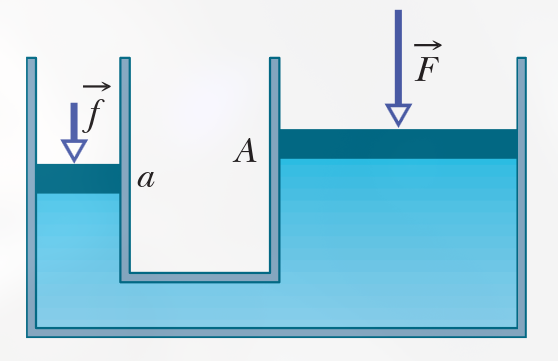
\includegraphics[width=0.45\linewidth]{images/28.png}
  \caption{Ilustrasi Tekanan Hidrolik nomor 28}
  \label{fig:hydraulic-press}
\end{figure}
 
\diketahui
\begin{align*}
d_k &= \SI{3,80}{\centi\metre}, &
d_b &= \SI{53,0}{\centi\metre}, &
F &= \SI{20,0}{\kilo\newton} = \SI{2,00e4}{\newton}
\end{align*}
 
\ditanya\ (a) $F$ dalam $f$, $a$, $A$; (b) $f$ pada piston kecil.
 
\konsep\ Prinsip Pascal: pertambahan tekanan pada fluida tertutup diteruskan sama besar ke
seluruh bagian fluida, sehingga $f/a = F/A$.
 
\penyelesaian
 
\textbf{(a)}
\begin{equation}
\frac{f}{a} = \frac{F}{A} \quad\Longrightarrow\quad F = f\,\frac{A}{a}
\end{equation}
Karena $A > a$, gaya kecil $f$ dapat menyeimbangkan gaya besar $F$.
 
\textbf{(b)} Luas piston sebanding dengan kuadrat diameter ($A = \pi d^2/4$), sehingga
\begin{align}
f &= F\,\frac{a}{A} = F \left(\frac{d_k}{d_b}\right)^2
 = (\SI{2,00e4}{\newton})\left(\frac{\SI{3,80}{\centi\metre}}{\SI{53,0}{\centi\metre}}\right)^2 \\
 &= (\SI{2,00e4}{\newton})(\num{5,14e-3}) = \SI{1,03e2}{\newton}
\end{align}
 
\begin{jawaban}
(a) $F = f\,A/a$.\\
(b) $f \approx \SI{1,03e2}{\newton}$.
\end{jawaban}

\soal{32}
Pada Gambar 14-38, sebuah kubus bersisi $L = \SI{0,600}{\metre}$ dan bermassa
$\SI{450}{\kilo\gram}$ digantung dengan tali di dalam tangki terbuka berisi cairan bermassa
jenis $\SI{1030}{\kilo\gram\per\metre\cubed}$. Tentukan (a) besar gaya total ke bawah pada
sisi atas kubus dari cairan dan atmosfer (tekanan atmosfer $\SI{1,00}{\atm}$),
(b) besar gaya total ke atas pada sisi bawah kubus, dan (c) tegangan tali.
(d) Hitung gaya apung dengan prinsip Archimedes. Hubungan apa yang berlaku di antara
semua besaran tersebut?

\begin{figure}[H]
  \centering
  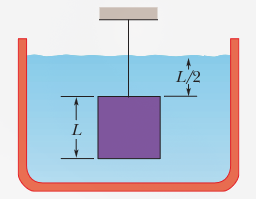
\includegraphics[width=0.45\linewidth]{images/32.png}
  \caption{Ilustrasi Kubus dalam Cairan nomor 32}
  \label{fig:cube}
\end{figure}
 
\diketahui\ (dari Gambar 14-38, sisi atas kubus berada $L/2$ di bawah permukaan cairan)
\begin{align*}
L &= \SI{0,600}{\metre}, &
m &= \SI{450}{\kilo\gram}, &
\rho &= \SI{1030}{\kilo\gram\per\metre\cubed}\\
p_0 &= \SI{1,00}{\atm} = \SI{1,013e5}{\pascal}, &
A &= L^2 = \SI{0,360}{\metre\squared}
\end{align*}
 
\ditanya\ (a) $F_{\text{atas}}$; (b) $F_{\text{bawah}}$; (c) $T$; (d) $F_b$.
 
\konsep\ Tekanan pada kedalaman $y$: $p = p_0 + \rho g y$. Sisi atas berada pada kedalaman
$L/2 = \SI{0,300}{\metre}$ dan sisi bawah pada $3L/2 = \SI{0,900}{\metre}$.
 
\penyelesaian
 
\textbf{(a)} Gaya pada sisi atas:
\begin{align}
p_{\text{atas}} &= p_0 + \rho g \tfrac{L}{2}
 = \SI{1,013e5}{\pascal} + (\num{1030})(\num{9,8})(\num{0,300}) = \SI{1,043e5}{\pascal} \\
F_{\text{atas}} &= p_{\text{atas}} A = (\SI{1,043e5}{\pascal})(\SI{0,360}{\metre\squared}) = \SI{3,76e4}{\newton}
\end{align}
 
\textbf{(b)} Gaya pada sisi bawah:
\begin{align}
p_{\text{bawah}} &= p_0 + \rho g \tfrac{3L}{2}
 = \SI{1,013e5}{\pascal} + (\num{1030})(\num{9,8})(\num{0,900}) = \SI{1,104e5}{\pascal} \\
F_{\text{bawah}} &= p_{\text{bawah}} A = (\SI{1,104e5}{\pascal})(\SI{0,360}{\metre\squared}) = \SI{3,97e4}{\newton}
\end{align}
 
\textbf{(c)} Kubus setimbang: $T + F_{\text{bawah}} = mg + F_{\text{atas}}$, sehingga
\begin{align}
T &= mg - \left(F_{\text{bawah}} - F_{\text{atas}}\right) \\
  &= (\num{450})(\num{9,8}) - \left(\SI{3,974e4}{\newton} - \SI{3,756e4}{\newton}\right) \\
  &= \SI{4410}{\newton} - \SI{2180}{\newton} = \SI{2,23e3}{\newton}
\end{align}
 
\textbf{(d)} Gaya apung menurut Archimedes (berat cairan yang dipindahkan):
\begin{equation}
F_b = \rho g V = \rho g L^3 = (\num{1030})(\num{9,8})(\num{0,600})^3 = \SI{2,18e3}{\newton}
\end{equation}
 
\textbf{Hubungan:} Gaya apung sama dengan selisih gaya tekan pada sisi bawah dan sisi atas,
$F_b = F_{\text{bawah}} - F_{\text{atas}}$, dan tegangan tali memenuhi $T = mg - F_b$.
 
\begin{jawaban}
(a) $F_{\text{atas}} \approx \SI{3,76e4}{\newton}$.\\
(b) $F_{\text{bawah}} \approx \SI{3,97e4}{\newton}$.\\
(c) $T \approx \SI{2,23e3}{\newton}$.\\
(d) $F_b \approx \SI{2,18e3}{\newton} = F_{\text{bawah}} - F_{\text{atas}}$.
\end{jawaban}

\soal{33}
Sebuah jangkar besi bermassa jenis $\SI{7870}{\kilo\gram\per\metre\cubed}$ tampak lebih ringan
$\SI{200}{\newton}$ di dalam air dibandingkan di udara. (a) Berapa volume jangkar?
(b) Berapa berat jangkar di udara?
 
\diketahui
\begin{align*}
\rho_{\text{besi}} &= \SI{7870}{\kilo\gram\per\metre\cubed}, &
\Delta W &= \SI{200}{\newton}, &
\rho_{\text{air}} &= \SI{1,00e3}{\kilo\gram\per\metre\cubed}
\end{align*}
 
\ditanya\ (a) $V$; (b) $W_{\text{udara}}$.
 
\konsep\ Berat semu di air lebih kecil daripada berat di udara sebesar gaya apung:
$\Delta W = F_b = \rho_{\text{air}}\, g\, V$.
 
\penyelesaian
 
\textbf{(a)}
\begin{equation}
V = \frac{F_b}{\rho_{\text{air}}\, g} = \frac{\SI{200}{\newton}}{(\SI{1,00e3}{\kilo\gram\per\metre\cubed})(\SI{9,8}{\meter\per\second\squared})}
 = \SI{2,04e-2}{\metre\cubed}
\end{equation}
 
\textbf{(b)}
\begin{equation}
W_{\text{udara}} = \rho_{\text{besi}}\, g\, V = (\num{7870})(\num{9,8})(\num{2,04e-2}) = \SI{1,57e3}{\newton}
\end{equation}
 
\begin{jawaban}
(a) $V \approx \SI{2,04e-2}{\metre\cubed}$.\\
(b) $W_{\text{udara}} \approx \SI{1,57e3}{\newton}$.
\end{jawaban}

\soal{62}
Sebuah \textit{tabung pitot} (Gambar 14-48) dipakai untuk menentukan kelajuan udara sebuah
pesawat. Alat ini terdiri atas tabung luar dengan sejumlah lubang kecil $B$ (empat lubang
ditunjukkan) yang memungkinkan udara masuk ke dalam tabung; tabung itu terhubung ke satu
lengan pipa-U. Lengan lain pipa-U terhubung ke lubang $A$ di ujung depan alat, yang menghadap
ke arah gerak pesawat. Di $A$ udara menjadi diam sehingga $v_A = 0$. Namun di $B$, kelajuan
udara dianggap sama dengan kelajuan udara $v$ pesawat. (a) Gunakan persamaan Bernoulli untuk
menunjukkan bahwa
\begin{equation*}
v = \sqrt{\frac{2\rho g h}{\rho_{\text{udara}}}}
\end{equation*}
dengan $\rho$ massa jenis cairan dalam pipa-U dan $h$ selisih tinggi permukaan cairan.
(b) Misalkan tabung berisi alkohol dan selisih tinggi $h = \SI{26,0}{\centi\metre}$. Berapa
kelajuan pesawat relatif terhadap udara? Massa jenis udara $\SI{1,03}{\kilo\gram\per\metre\cubed}$
dan alkohol $\SI{810}{\kilo\gram\per\metre\cubed}$.

\begin{figure}[H]
  \centering
  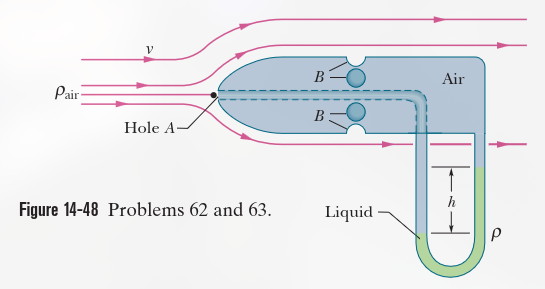
\includegraphics[width=0.45\linewidth]{images/62.png}
  \caption{Ilustrasi Tabung Pitot nomor 62 (juga dipakai pada Soal 63)}
  \label{fig:pitot-tube}
\end{figure}

\diketahui
\begin{align*}
\rho_{\text{alkohol}} &= \SI{810}{\kilo\gram\per\metre\cubed}, &
\rho_{\text{udara}} &= \SI{1,03}{\kilo\gram\per\metre\cubed}, &
h &= \SI{26,0}{\centi\metre} = \SI{0,260}{\metre}
\end{align*}

\ditanya\ (a) Pembuktian rumus $v$; (b) nilai $v$.

\konsep\ Titik $A$ (kelajuan nol) dan titik $B$ (kelajuan $v$) berada pada ketinggian yang
sama. Selisih tekanan di antara keduanya ditunjukkan oleh selisih tinggi cairan dalam pipa-U:
$p_A - p_B = \rho g h$.

\penyelesaian

\textbf{(a)} Bernoulli antara $A$ dan $B$:
\begin{align}
p_A + \tfrac{1}{2}\rho_{\text{udara}}(0)^2 &= p_B + \tfrac{1}{2}\rho_{\text{udara}}\, v^2 \\
p_A - p_B &= \tfrac{1}{2}\rho_{\text{udara}}\, v^2
\end{align}
Karena $p_A - p_B = \rho g h$,
\begin{equation}
\rho g h = \tfrac{1}{2}\rho_{\text{udara}}\, v^2
\ \Longrightarrow\
v = \sqrt{\frac{2\rho g h}{\rho_{\text{udara}}}} \qquad \blacksquare
\end{equation}

\textbf{(b)}
\begin{equation}
v = \sqrt{\frac{2(\num{810})(\num{9,8})(\num{0,260})}{\num{1,03}}} = \SI{63,3}{\meter\per\second}
\end{equation}

\begin{jawaban}
(a) $v = \sqrt{2\rho g h/\rho_{\text{udara}}}$ (terbukti).\\
(b) $v \approx \SI{63,3}{\meter\per\second}$.
\end{jawaban}

\soal{63}
Sebuah tabung pitot (lihat Soal 62 dan gambarnya) pada pesawat berketinggian tinggi mengukur
selisih tekanan $\SI{180}{\pascal}$. Berapa kelajuan udara pesawat jika massa jenis udara
$\SI{0,031}{\kilo\gram\per\metre\cubed}$?

\diketahui
\begin{align*}
\Delta p &= \SI{180}{\pascal}, &
\rho_{\text{udara}} &= \SI{0,031}{\kilo\gram\per\metre\cubed}
\end{align*}

\ditanya\ Kelajuan udara $v$.

\konsep\ Dari Soal 62, selisih tekanan antara titik stagnasi dan titik aliran bebas adalah
$\Delta p = \tfrac{1}{2}\rho_{\text{udara}}\, v^2$.

\penyelesaian
\begin{equation}
v = \sqrt{\frac{2\,\Delta p}{\rho_{\text{udara}}}} = \sqrt{\frac{2(\num{180})}{\num{0,031}}} = \SI{1,1e2}{\meter\per\second}
\end{equation}

\begin{jawaban}
$v \approx \SI{1,1e2}{\meter\per\second}$ (tepatnya $\SI{108}{\meter\per\second}$).
\end{jawaban}

\soal{64}
Pada Gambar 14-49, air mengalir melalui pipa horizontal lalu keluar ke atmosfer dengan
kelajuan $v_1 = \SI{15}{\meter\per\second}$. Diameter bagian pipa kiri dan kanan berturut-turut
$\SI{5,0}{\centi\metre}$ dan $\SI{3,0}{\centi\metre}$. (a) Berapa volume air yang mengalir
ke atmosfer selama $\SI{10}{\minute}$? Pada bagian kiri pipa, berapa (b) kelajuan $v_2$ dan
(c) tekanan gauge?

\begin{figure}[H]
  \centering
  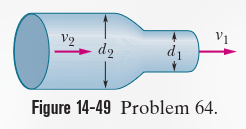
\includegraphics[width=0.45\linewidth]{images/64.png}
  \caption{Ilustrasi Aliran Air pada Pipa yang Menyempit nomor 64}
  \label{fig:pipa-menyempit}
\end{figure}

\diketahui
\begin{align*}
v_1 &= \SI{15}{\meter\per\second}, &
d_1 &= \SI{3,0}{\centi\metre}\ (\text{kanan}), &
d_2 &= \SI{5,0}{\centi\metre}\ (\text{kiri}), &
t &= \SI{10}{\minute} = \SI{600}{\second}
\end{align*}

\ditanya\ (a) $V$; (b) $v_2$; (c) $p_{g,2}$.

\konsep\ Debit $Q = A_1 v_1$; kontinuitas $A_1 v_1 = A_2 v_2$; Bernoulli untuk pipa horizontal
dengan tekanan di ujung keluar sama dengan tekanan atmosfer ($p_{g,1} = 0$).

\penyelesaian

\textbf{(a)}
\begin{align}
A_1 &= \pi\left(\frac{d_1}{2}\right)^2 = \pi(\SI{1,5e-2}{\metre})^2 = \SI{7,07e-4}{\metre\squared} \\
V &= A_1 v_1\, t = (\SI{7,07e-4}{\metre\squared})(\SI{15}{\meter\per\second})(\SI{600}{\second}) = \SI{6,4}{\metre\cubed}
\end{align}

\textbf{(b)}
\begin{equation}
v_2 = v_1\left(\frac{d_1}{d_2}\right)^2 = (\SI{15}{\meter\per\second})\left(\frac{\num{3,0}}{\num{5,0}}\right)^2 = \SI{5,4}{\meter\per\second}
\end{equation}

\textbf{(c)}
\begin{align}
p_{g,2} &= p_2 - p_0 = \tfrac{1}{2}\rho\left(v_1^2 - v_2^2\right) \\
 &= \tfrac{1}{2}(\num{1,00e3})\left[(\num{15})^2 - (\num{5,4})^2\right] = \SI{9,8e4}{\pascal}
\end{align}

\begin{jawaban}
(a) $V \approx \SI{6,4}{\metre\cubed}$.\\
(b) $v_2 \approx \SI{5,4}{\meter\per\second}$.\\
(c) $p_{g,2} \approx \SI{9,8e4}{\pascal}$.
\end{jawaban}

\soal{65}
Sebuah \textit{venturimeter} dipakai untuk mengukur kelajuan aliran fluida dalam pipa. Alat ini
dipasang di antara dua bagian pipa (Gambar 14-50); luas penampang $A$ pada pintu masuk dan
keluar alat sama dengan luas penampang pipa. Di antara pintu masuk dan keluar, fluida mengalir
dari pipa dengan kelajuan $V$ lalu melalui ``leher'' sempit berluas penampang $a$ dengan
kelajuan $v$. Sebuah manometer menghubungkan bagian lebar dengan bagian sempit. Perubahan
kelajuan fluida disertai perubahan tekanan $\Delta p$ (tekanan di leher dikurangi tekanan di
pipa), yang menyebabkan selisih tinggi $h$ cairan pada kedua lengan manometer. (a) Dengan
Bernoulli dan persamaan kontinuitas pada titik 1 dan 2, tunjukkan bahwa
\begin{equation*}
V = \sqrt{\frac{2a^2\,\Delta p}{\rho\,(a^2 - A^2)}}
\end{equation*}
dengan $\rho$ massa jenis fluida. (b) Misalkan fluida adalah air tawar, luas penampang pipa
$\SI{64}{\centi\metre\squared}$ dan leher $\SI{32}{\centi\metre\squared}$, tekanan di pipa
$\SI{55}{\kilo\pascal}$ dan di leher $\SI{41}{\kilo\pascal}$. Berapa laju aliran air dalam
meter kubik per detik?

\begin{figure}[H]
  \centering
  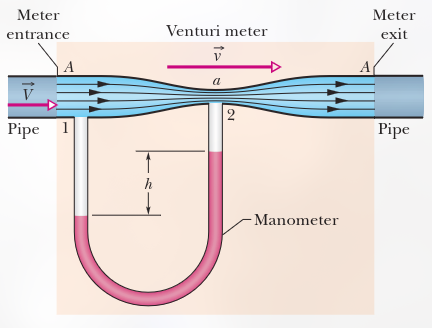
\includegraphics[width=0.45\linewidth]{images/65.png}
  \caption{Ilustrasi Venturimeter nomor 65 (juga dipakai pada Soal 66)}
  \label{fig:venturimeter}
\end{figure}

\diketahui
\begin{align*}
A &= \SI{64}{\centi\metre\squared} = \SI{6,4e-3}{\metre\squared}, &
a &= \SI{32}{\centi\metre\squared} = \SI{3,2e-3}{\metre\squared}\\
p_1 &= \SI{55}{\kilo\pascal}, &
p_2 &= \SI{41}{\kilo\pascal}\\
\rho &= \SI{1,00e3}{\kilo\gram\per\metre\cubed}
\end{align*}

\ditanya\ (a) Pembuktian rumus $V$; (b) laju aliran volume $R_V = A V$.

\konsep\ Titik 1 (pipa, kelajuan $V$, tekanan $p_1$) dan titik 2 (leher, kelajuan $v$,
tekanan $p_2$) berada pada ketinggian sama. Gunakan kontinuitas $A V = a v$ dan Bernoulli.

\penyelesaian

\textbf{(a)} Dari kontinuitas, $v = (A/a)\,V$. Bernoulli:
\begin{align}
p_1 + \tfrac{1}{2}\rho V^2 &= p_2 + \tfrac{1}{2}\rho v^2 \\
\Delta p = p_2 - p_1 &= \tfrac{1}{2}\rho\left(V^2 - v^2\right)
 = \tfrac{1}{2}\rho V^2\left(1 - \frac{A^2}{a^2}\right) = \frac{\rho V^2\,(a^2 - A^2)}{2a^2}
\end{align}
Menyelesaikan untuk $V$:
\begin{equation}
V = \sqrt{\frac{2a^2\,\Delta p}{\rho\,(a^2 - A^2)}} \qquad \blacksquare
\end{equation}
(Karena $a < A$, baik $\Delta p$ maupun $a^2 - A^2$ bernilai negatif sehingga $V^2 > 0$.)

\textbf{(b)}
\begin{align}
\Delta p &= \SI{41}{\kilo\pascal} - \SI{55}{\kilo\pascal} = -\SI{1,4e4}{\pascal} \\
V &= \sqrt{\frac{2(\SI{3,2e-3}{\metre\squared})^2(-\SI{1,4e4}{\pascal})}{(\SI{1,00e3}{\kilo\gram\per\metre\cubed})\left[(\SI{3,2e-3}{\metre\squared})^2 - (\SI{6,4e-3}{\metre\squared})^2\right]}}
 = \SI{3,06}{\meter\per\second} \\
R_V &= A V = (\SI{6,4e-3}{\metre\squared})(\SI{3,06}{\meter\per\second}) = \SI{2,0e-2}{\metre\cubed\per\second}
\end{align}

\begin{jawaban}
(a) $V = \sqrt{2a^2\Delta p/[\rho(a^2 - A^2)]}$ (terbukti).\\
(b) $R_V \approx \SI{2,0e-2}{\metre\cubed\per\second}$.
\end{jawaban}

\soal{66}
Tinjau tabung venturi pada Soal 65 dan Gambar 14-50 tanpa manometer. Misalkan $A$ sama
dengan $5a$. Tekanan $p_1$ di $A$ adalah $\SI{2,0}{\atm}$. Hitung (a) kelajuan $V$ di $A$ dan
(b) kelajuan $v$ di $a$ yang membuat tekanan $p_2$ di $a$ sama dengan nol. (c) Hitung laju
aliran volume yang bersesuaian jika diameter di $A$ adalah $\SI{5,0}{\centi\metre}$. Gejala
yang terjadi di $a$ ketika $p_2$ turun hingga hampir nol dikenal sebagai \textit{kavitasi}:
air menguap menjadi gelembung-gelembung kecil.

\diketahui
\begin{align*}
A &= 5a, &
p_1 &= \SI{2,0}{\atm} = \SI{2,03e5}{\pascal}, &
p_2 &= 0\\
d_A &= \SI{5,0}{\centi\metre}, &
\rho &= \SI{1,00e3}{\kilo\gram\per\metre\cubed}
\end{align*}

\ditanya\ (a) $V$; (b) $v$; (c) $R_V$.

\konsep\ Kontinuitas $A V = a v$ memberi $v = (A/a)\,V = 5V$. Bernoulli pada
ketinggian yang sama:
$p_1 + \tfrac{1}{2}\rho V^2 = p_2 + \tfrac{1}{2}\rho v^2$.

\penyelesaian

\textbf{(a)} Dengan $p_2 = 0$ dan $v = 5V$:
\begin{align}
p_1 &= \tfrac{1}{2}\rho\left[(5V)^2 - V^2\right] = 12\,\rho V^2 \\
V &= \sqrt{\frac{p_1}{12\rho}} = \sqrt{\frac{\SI{2,03e5}{\pascal}}{12(\SI{1,00e3}{\kilo\gram\per\metre\cubed})}} = \SI{4,1}{\meter\per\second}
\end{align}

\textbf{(b)}
\begin{equation}
v = 5V = 5(\SI{4,11}{\meter\per\second}) = \SI{21}{\meter\per\second}
\end{equation}

\textbf{(c)}
\begin{equation}
R_V = A V = \pi\left(\SI{2,5e-2}{\metre}\right)^2(\SI{4,11}{\meter\per\second}) = \SI{8,1e-3}{\metre\cubed\per\second}
\end{equation}

\begin{jawaban}
(a) $V \approx \SI{4,1}{\meter\per\second}$.\\
(b) $v \approx \SI{21}{\meter\per\second}$.\\
(c) $R_V \approx \SI{8,1e-3}{\metre\cubed\per\second}$.
\end{jawaban}

\soal{71}
Gambar 14-54 menunjukkan aliran air melalui lubang pada kedalaman $h = \SI{10}{\centi\meter}$
dalam tangki berisi air setinggi $H = \SI{40}{\centi\meter}$.
(a) Pada jarak $x$ berapa aliran air menyentuh lantai?
(b) Pada kedalaman berapa lubang kedua harus dibuat agar menghasilkan nilai $x$ yang sama?
(c) Pada kedalaman berapa lubang harus dibuat agar $x$ maksimum?
 
\begin{figure}[H]
  \centering
  \IfFileExists{images/26.png}
    {\includegraphics[width=0.35\linewidth]{images/26.png}}
    {\fbox{\parbox{0.35\linewidth}{\centering Gambar 14-54}}}
  \caption{Ilustrasi aliran air dari lubang tangki nomor 71}
  \label{fig:tangki-lubang}
\end{figure}
 
\diketahui
\begin{align*}
h &= \SI{10}{\centi\meter} = \SI{0,10}{\meter}, &
H &= \SI{40}{\centi\meter} = \SI{0,40}{\meter}
\end{align*}
 
\ditanya\ (a) $x$; (b) kedalaman lubang kedua $h'$ untuk $x$ yang sama; (c) $h$ untuk $x$ maksimum.
 
\konsep\ Kelajuan semburan di lubang mengikuti teorema Torricelli, $v = \sqrt{2gh}$
(Bernoulli antara permukaan air dan lubang). Setelah keluar, air bergerak sebagai gerak
parabola dengan kecepatan awal horizontal $v$ dari ketinggian $H-h$ di atas lantai, sehingga
waktu jatuh $t = \sqrt{2(H-h)/g}$ dan jarak horizontal $x = vt$.
 
\penyelesaian
 
\textbf{(a)} Jarak jangkauan secara umum:
\begin{align*}
x = vt = \sqrt{2gh}\,\sqrt{\frac{2(H-h)}{g}} = 2\sqrt{h\,(H-h)}
\end{align*}
Dengan data soal:
\begin{align*}
x = 2\sqrt{(\num{0,10})(\num{0,40}-\num{0,10})}\ \si{\meter}
  = 2\sqrt{\num{0,030}}\ \si{\meter} = \SI{0,35}{\meter}
\end{align*}
 
\textbf{(b)} Nilai $x$ sama bila $h'(H-h') = h(H-h)$. Persamaan kuadrat
$h'^2 - Hh' + h(H-h) = 0$ memiliki dua akar, yaitu $h' = h$ dan $h' = H - h$. Jadi
\begin{align*}
h' = H - h = \SI{40}{\centi\meter} - \SI{10}{\centi\meter} = \SI{30}{\centi\meter}
\end{align*}
 
\textbf{(c)} $x$ maksimum bila $h(H-h)$ maksimum:
\begin{align*}
\frac{d}{dh}\left[h(H-h)\right] = H - 2h = 0 \quad\Rightarrow\quad h = \frac{H}{2} = \SI{20}{\centi\meter}
\end{align*}
Pada kedalaman ini $x_{\text{maks}} = 2\sqrt{(H/2)^2} = H = \SI{0,40}{\meter}$.
 
\begin{jawaban}
(a) $x \approx \SI{0,35}{\meter}$ \quad (b) $h' = \SI{30}{\centi\meter}$ (simetris terhadap $h$ terhadap titik $H/2$)
\quad (c) $h = \SI{20}{\centi\meter}$, dengan $x_{\text{maks}} = \SI{0,40}{\meter}$.
\end{jawaban}

\soal{72}
Gambar 14-55 menunjukkan sistem drainase air hujan yang disederhanakan untuk sebuah rumah.
Air hujan dari atap mengalir ke talang, lalu melalui pipa tegak (\textit{downspout}) menuju
pipa drainase utama $M$ di bawah ruang bawah tanah. Saluran lantai di ruang bawah tanah juga
terhubung ke pipa $M$. Anggap: (1) tinggi pipa tegak $h_1 = \SI{11}{\meter}$;
(2) tinggi saluran lantai $h_2 = \SI{1,2}{\meter}$; (3) jari-jari pipa $M$ adalah $\SI{3,0}{\centi\meter}$;
(4) lebar sisi rumah $w = \SI{30}{\meter}$ dan panjang muka $L = \SI{60}{\meter}$;
(5) seluruh air hujan yang mengenai atap masuk ke pipa $M$; (6) kelajuan awal air di pipa tegak
dapat diabaikan; (7) kelajuan angin dapat diabaikan (hujan jatuh vertikal).
Pada laju curah hujan berapa (dalam cm/jam) air dari pipa $M$ mencapai ketinggian saluran lantai
dan mengancam membanjiri ruang bawah tanah?
 
\begin{figure}[H]
  \centering
  \IfFileExists{images/27.png}
    {\includegraphics[width=0.4\linewidth]{images/27.png}}
    {\fbox{\parbox{0.4\linewidth}{\centering Gambar 14-55}}}
  \caption{Skema sistem drainase air hujan nomor 72}
  \label{fig:drainase}
\end{figure}
 
\diketahui
\begin{align*}
h_1 &= \SI{11}{\meter}, & h_2 &= \SI{1,2}{\meter}, & r_M &= \SI{3,0}{\centi\meter} = \SI{0,030}{\meter}, \\
w &= \SI{30}{\meter}, & L &= \SI{60}{\meter}, & \rho &= \SI{1,00e3}{\kilo\gram\per\metre\cubed}
\end{align*}
 
\ditanya\ Laju curah hujan $R$ (cm/jam) saat air di pipa $M$ mencapai ketinggian saluran lantai.
 
\konsep\ Air mulai meluap ke saluran lantai ketika tekanan di pipa $M$ pada ketinggian $h_2$
sama dengan tekanan atmosfer $p_0$. Persamaan Bernoulli diterapkan antara puncak pipa tegak
(tekanan $p_0$, kelajuan $\approx 0$, ketinggian $h_1$ di atas pipa $M$) dan titik di pipa $M$
pada ketinggian $h_2$ (tekanan $p_0$, kelajuan $v$). Kekekalan debit menghubungkan $v$ dengan
laju curah hujan: $R\,(wL) = A_M v$.
 
\penyelesaian
 
Bernoulli:
\begin{align*}
p_0 + \rho g h_1 + 0 &= p_0 + \rho g h_2 + \tfrac{1}{2}\rho v^2 \\
v &= \sqrt{2g(h_1 - h_2)} = \sqrt{2(\num{9,8})(\num{11}-\num{1,2})}\ \si{\meter\per\second} = \SI{13,9}{\meter\per\second}
\end{align*}
Debit air di pipa $M$:
\begin{align*}
Q = A_M v = \pi r_M^2 v = \pi(\num{0,030})^2(\num{13,86})\ \si{\metre\cubed\per\second} = \SI{3,92e-2}{\metre\cubed\per\second}
\end{align*}
Laju curah hujan (volume air per satuan waktu per luas atap $wL$):
\begin{align*}
R &= \frac{Q}{wL} = \frac{\num{3,92e-2}}{(30)(60)}\ \si{\meter\per\second}
  = \SI{2,18e-5}{\meter\per\second}\\
  &= \left(\num{2,18e-5}\right)\left(\num{3,6e5}\right)\ \si{\centi\meter\per\hour}
  \approx \SI{7,8}{\centi\meter\per\hour}
\end{align*}
 
\begin{jawaban}
$R \approx \SI{7,8}{\centi\meter\per\hour}$
\end{jawaban}

\soal{79}
Sebuah benda digantung pada neraca pegas. Neraca menunjukkan $\SI{30}{\newton}$ di udara,
$\SI{20}{\newton}$ ketika benda dicelupkan ke dalam air, dan $\SI{24}{\newton}$ ketika benda dicelupkan ke dalam
cairan lain yang massa jenisnya tidak diketahui. Berapakah massa jenis cairan lain tersebut?
 
\diketahui
\begin{align*}
W_{\text{udara}} = \SI{30}{\newton}, \quad
W_{\text{air}} = \SI{20}{\newton}, \quad
W_{\text{cairan}} = \SI{24}{\newton}, \quad
\rho_{\text{air}} = \SI{1,00e3}{\kilo\gram\per\metre\cubed}
\end{align*}
 
\ditanya\ Massa jenis cairan $\rho_x$.
 
\konsep\ Bacaan neraca pegas pada benda yang tercelup adalah berat semu, $W_{\text{app}} = W - F_b$.
Dengan benda yang sama tercelup penuh, volume fluida yang dipindahkan sama, sehingga gaya apung
sebanding dengan massa jenis fluida: $F_b = \rho_f V g$.
 
\penyelesaian
 
Gaya apung pada tiap fluida:
\begin{align*}
F_{b,\text{air}} &= 30 - 20 = \SI{10}{\newton}, &
F_{b,x} &= 30 - 24 = \SI{6}{\newton}
\end{align*}
Perbandingan kedua gaya apung memberikan
\begin{align*}
\frac{\rho_x}{\rho_{\text{air}}} = \frac{F_{b,x}}{F_{b,\text{air}}} = \frac{6}{10} = 0{,}60
\quad\Rightarrow\quad
\rho_x = 0{,}60\,(\SI{1,00e3}{\kilo\gram\per\metre\cubed}) = \SI{6,0e2}{\kilo\gram\per\metre\cubed}
\end{align*}
 
\begin{jawaban}
$\rho_x = \SI{6,0e2}{\kilo\gram\per\metre\cubed} = \SI{0,60}{\gram\per\centi\meter\cubed}$
\end{jawaban}

\soal{80}
Dalam sebuah percobaan, sebuah balok persegi panjang setinggi $h$ dibiarkan mengapung dalam empat cairan
berbeda. Pada cairan pertama, yaitu air, balok mengapung dengan tercelup sepenuhnya. Pada cairan $A$, $B$,
dan $C$, balok mengapung dengan tinggi $h/2$, $2h/3$, dan $h/4$ di atas permukaan cairan.
Berapakah massa jenis relatif (massa jenis terhadap air) dari (a) $A$, (b) $B$, dan (c) $C$?
 
\diketahui
\begin{align*}
h_{\text{atas},A} = \frac{h}{2}, \qquad
h_{\text{atas},B} = \frac{2h}{3}, \qquad
h_{\text{atas},C} = \frac{h}{4}
\end{align*}
Pada air, balok tercelup seluruhnya ($V_{\text{tc}} = V$).
 
\ditanya\ Massa jenis relatif $\rho_A/\rho_{\text{air}}$, $\rho_B/\rho_{\text{air}}$, dan $\rho_C/\rho_{\text{air}}$.
 
\konsep\ Karena balok mengapung tepat tercelup seluruhnya di air, massa jenis balok sama dengan massa jenis air:
$\rho_{\text{balok}} = \rho_{\text{air}}$. Untuk cairan mana pun, kesetimbangan apung memberikan
$\rho_f V_{\text{tc}} = \rho_{\text{balok}} V$. Karena penampang balok seragam, fraksi volume
tercelup sama dengan fraksi tinggi tercelup:
\begin{align*}
\frac{\rho_f}{\rho_{\text{air}}} = \frac{V}{V_{\text{tc}}} = \frac{h}{h_{\text{tc}}}
\end{align*}
 
\penyelesaian
 
\textbf{(a)} Cairan $A$: $h_{\text{tc}} = h - \dfrac{h}{2} = \dfrac{h}{2}$
\begin{align*}
\frac{\rho_A}{\rho_{\text{air}}} = \frac{h}{h/2} = 2{,}00
\end{align*}
 
\textbf{(b)} Cairan $B$: $h_{\text{tc}} = h - \dfrac{2h}{3} = \dfrac{h}{3}$
\begin{align*}
\frac{\rho_B}{\rho_{\text{air}}} = \frac{h}{h/3} = 3{,}00
\end{align*}
 
\textbf{(c)} Cairan $C$: $h_{\text{tc}} = h - \dfrac{h}{4} = \dfrac{3h}{4}$
\begin{align*}
\frac{\rho_C}{\rho_{\text{air}}} = \frac{h}{3h/4} = \frac{4}{3} = 1{,}33
\end{align*}
 
\begin{jawaban}
(a) $\rho_A/\rho_{\text{air}} = 2{,}00$ \quad (b) $\rho_B/\rho_{\text{air}} = 3{,}00$ \quad (c) $\rho_C/\rho_{\text{air}} \approx 1{,}33$
\end{jawaban}

\soal{83}
Sebuah sifon digunakan untuk mengalirkan cairan bermassa jenis $\rho=\SI{1000}{\kilogram\per\metre\cubed}$. Diketahui $h_1=\SI{25}{\centi\metre}$, $d=\SI{12}{\centi\metre}$, dan $h_2=\SI{40}{\centi\metre}$. Anggap viskositas dapat diabaikan. Tentukan (a) kelajuan cairan saat keluar di titik C, (b) tekanan di titik tertinggi B jika tekanan atmosfer \SI{1,0e5}{\pascal}, dan (c) nilai maksimum teoretis $h_1$.

\begin{figure}[H]
  \centering
  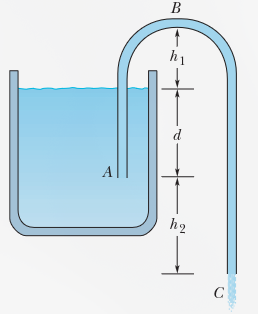
\includegraphics[width=0.45\linewidth]{images/83.png}
  \caption{Ilustrasi sifon nomor 83}
  \label{fig:sifon}
\end{figure}

\diketahui\ (dari gambar: $h_1$ = tinggi B di atas permukaan cairan; $d$ = kedalaman ujung tabung A di bawah permukaan; $h_2$ = jarak vertikal dari ujung A ke C)
\begin{align*}
\rho &= \SI{1000}{\kilogram\per\metre\cubed},&
h_1 &= \SI{0,25}{\metre},\\
d &= \SI{0,12}{\metre},&
h_2 &= \SI{0,40}{\metre},\\
p_{\mathrm{atm}} &= \SI{1,0e5}{\pascal}.
\end{align*}
\ditanya\ (a) Kelajuan di C, $v_C$; (b) tekanan di B, $p_B$; (c) $h_{1,\max}$.

\konsep\ Gunakan persamaan Bernoulli antara permukaan bebas cairan (kelajuan dianggap nol, tekanan $p_{\mathrm{atm}}$) dan titik keluaran C (tekanan $p_{\mathrm{atm}}$). Titik C berada $d+h_2$ di bawah permukaan cairan. Karena penampang tabung seragam, kelajuan cairan di seluruh tabung sama dengan $v_C$ (kontinuitas). Untuk titik B, Bernoulli diterapkan antara permukaan bebas dan B, yang berada $h_1$ di atas permukaan. Nilai maksimum teoretis $h_1$ diperoleh dari batas tekanan absolut di B sama dengan nol.

\penyelesaian

\noindent\textbf{(a) Kelajuan cairan di C}
\begin{align*}
p_{\mathrm{atm}}+\rho g (d+h_2)
&=p_{\mathrm{atm}}+\frac12\rho v_C^2,\\
v_C&=\sqrt{2g(d+h_2)}\\
&=\sqrt{2(\SI{9,8}{\metre\per\second\squared})(\SI{0,52}{\metre})}\\
&=\SI{3,2}{\metre\per\second}.
\end{align*}

\noindent\textbf{(b) Tekanan di titik B}
\begin{align*}
p_{\mathrm{atm}}
&=p_B+\rho g h_1+\frac12\rho v_C^2,\\
p_B&=p_{\mathrm{atm}}-\rho g h_1-\rho g(d+h_2)
=p_{\mathrm{atm}}-\rho g(h_1+d+h_2)\\
&=\SI{1,0e5}{\pascal}
-(\SI{1000}{\kilogram\per\metre\cubed})
(\SI{9,8}{\metre\per\second\squared})(\SI{0,77}{\metre})\\
&=\SI{9,25e4}{\pascal}.
\end{align*}

\noindent\textbf{(c) Ketinggian maksimum teoretis}
Pada batas teoretis $p_B=0$ (nilai $v_C$ tidak bergantung pada $h_1$):
\begin{align*}
0&=p_{\mathrm{atm}}-\rho g(h_{1,\max}+d+h_2),\\
h_{1,\max}&=\frac{p_{\mathrm{atm}}}{\rho g}-(d+h_2)\\
&=\frac{\SI{1,0e5}{\pascal}}
{(\SI{1000}{\kilogram\per\metre\cubed})(\SI{9,8}{\metre\per\second\squared})}
-\SI{0,52}{\metre}\\
&=\SI{10,2}{\metre}-\SI{0,52}{\metre}
=\SI{9,7}{\metre}.
\end{align*}
\begin{jawaban}
\[
\boxed{v_C\approx\SI{3,2}{\metre\per\second}},\qquad
\boxed{p_B\approx\SI{9,25e4}{\pascal}},\qquad
\boxed{h_{1,\max}\approx\SI{9,7}{\metre}}.
\]
Nilai maksimum pada (c) merupakan batas ideal ketika tekanan absolut di puncak sifon nol (sekitar $p_{\mathrm{atm}}/\rho g\approx\SI{10}{\metre}$ dikurangi $d+h_2$); pada keadaan nyata, tekanan uap cairan membatasi ketinggian lebih lanjut.
\end{jawaban}

\soal{86}
Sebuah balok padat ditahan oleh tali di bawah permukaan cairan yang massa jenisnya lebih besar daripada massa jenis balok. Saat wadah diam, tegangan tali adalah $T_0$. Tentukan tegangan tali ketika wadah dipercepat ke atas sebesar $0{,}250g$.

\diketahui
\begin{itemize}[nosep]
  \item Tegangan saat wadah diam: $T_0$
  \item Percepatan wadah: $a=0{,}250g$ ke atas
  \item Massa jenis cairan lebih besar daripada massa jenis balok
\end{itemize}

\ditanya Tegangan tali $T$ dalam kelipatan $T_0$.

\konsep Gaya apung dan berat efektif sama-sama sebanding dengan percepatan gravitasi efektif. Dalam kerangka wadah yang dipercepat ke atas, gravitasi efektifnya adalah
\[
g_{\mathrm{ef}}=g+a.
\]

\penyelesaian Saat wadah diam, gaya apung dikurangi berat balok sama dengan tegangan tali:
\[
T_0=(\rho_f-\rho_b)Vg.
\]
Ketika wadah dipercepat ke atas,
\[
T=(\rho_f-\rho_b)V(g+a).
\]
Membagi kedua persamaan menghasilkan
\[
\frac{T}{T_0}=\frac{g+a}{g}
=1+\frac{0{,}250g}{g}=1{,}250.
\]

\begin{jawaban}
\[
\boxed{T=1{,}25T_0}
\]
\end{jawaban}

\soal{88}
Sebuah bola bermassa \SI{8,60}{kg} dan berjari-jari \SI{6,22}{cm} berada pada kedalaman \SI{2,22}{km} di air laut dengan massa jenis rata-rata \SI{1025}{kg/m^3}. Tentukan (a) tekanan ukur, (b) tekanan total, (c) gaya total akibat tekanan yang menekan permukaan bola, (d) gaya apung, dan (e) besar percepatan bola jika bebas bergerak. Gunakan tekanan atmosfer \SI{1,01e5}{Pa}.

\diketahui
\begin{itemize}[nosep]
  \item $m=\SI{8,60}{kg}$
  \item $r=\SI{0,0622}{m}$
  \item $h=\SI{2220}{m}$
  \item $\rho=\SI{1025}{kg/m^3}$
  \item $p_{\mathrm{atm}}=\SI{1,01e5}{Pa}$
  \item $g=\SI{9,80}{m/s^2}$
\end{itemize}

\ditanya (a) $p_g$, (b) $p_{\mathrm{total}}$, (c) $F_p$, (d) $F_A$, dan (e) $a$.

\konsep Tekanan hidrostatik, gaya tekanan pada luas permukaan, prinsip Archimedes, dan Hukum II Newton digunakan.

\penyelesaian

\textbf{(a) Tekanan ukur}
\[
p_g=\rho gh
=(1025)(9{,}80)(2220)
\approx \SI{2,23e7}{Pa}.
\]
Jadi, $p_g\approx\SI{22,3}{MPa}$.

\textbf{(b) Tekanan total}
\[
p_{\mathrm{total}}=p_{\mathrm{atm}}+p_g
=1{,}01\times10^5+2{,}230\times10^7.
\]
\[
p_{\mathrm{total}}\approx\SI{2,24e7}{Pa}
=\SI{22,4}{MPa}.
\]

\textbf{(c) Gaya total akibat tekanan pada permukaan bola}

Luas permukaan bola adalah $A=4\pi r^2$, sehingga besar gaya tekanan total yang diminta dihitung dengan $F_p=p_{\mathrm{total}}A$:
\[
A=4\pi(0{,}0622)^2\approx\SI{0,0486}{m^2},
\]
\[
F_p=(2{,}240\times10^7)(0{,}0486)
\approx\SI{1,09e6}{N}.
\]

\textbf{(d) Gaya apung}

Volume bola:
\[
V=\frac{4}{3}\pi r^3
=\frac{4}{3}\pi(0{,}0622)^3
\approx\SI{1,008e-3}{m^3}.
\]
Dengan prinsip Archimedes,
\[
F_A=\rho Vg
=(1025)(1{,}008\times10^{-3})(9{,}80)
\approx\SI{10,1}{N}.
\]

\textbf{(e) Percepatan bola}

Berat bola adalah
\[
W=mg=(8{,}60)(9{,}80)=\SI{84,3}{N}.
\]
Karena $W>F_A$, resultan gaya mengarah ke bawah:
\[
F_{\mathrm{net}}=W-F_A=84{,}3-10{,}1=\SI{74,2}{N}.
\]
\[
a=\frac{F_{\mathrm{net}}}{m}
=\frac{74{,}2}{8{,}60}
\approx\SI{8,63}{m/s^2}.
\]

\begin{jawaban}
\[
\boxed{\begin{aligned}
\text{(a)}\;&p_g\approx\SI{2,23e7}{Pa}\\
\text{(b)}\;&p_{\mathrm{total}}\approx\SI{2,24e7}{Pa}\\
\text{(c)}\;&F_p\approx\SI{1,09e6}{N}\\
\text{(d)}\;&F_A\approx\SI{10,1}{N}\\
\text{(e)}\;&a\approx\SI{8,63}{m/s^2}\text{ ke bawah}
\end{aligned}}
\]
\end{jawaban}

\textit{Catatan:} Gaya pada (c) adalah tekanan total dikalikan luas permukaan bola, sesuai interpretasi besar gaya tekanan yang diminta. Secara fisik, tekanan seragam dari segala arah tidak menghasilkan resultan sebesar $pA$; resultan tekanan pada bola tertutup adalah gaya apung.

% =====================================================================
% BAB 15 -- OSILASI   (potongan untuk ditempel ke main.tex)
% Memakai makro yang sudah ada di main.tex: \bab, \soal, rumusutama,
% \diketahui, \ditanya, \konsep, \penyelesaian, jawaban.
% =====================================================================
\bab{15}{Osilasi}

\begin{rumusutama}
\begin{itemize}[nosep,leftmargin=*]
  \item \textbf{Besaran dasar:}
        $f = \dfrac{1}{T}$, \qquad $\omega = 2\pi f = \dfrac{2\pi}{T}$
  \item \textbf{Gerak harmonik sederhana (GHS):}
        $x(t) = x_m\cos(\omega t + \phi)$, \quad
        $v = -\omega x_m \sin(\omega t + \phi)$, \quad
        $a = -\omega^2 x$
  \item \textbf{Osilator pegas-benda:}
        $F = -kx$, \quad $\omega = \sqrt{\dfrac{k}{m}}$, \quad
        $T = 2\pi\sqrt{\dfrac{m}{k}}$
  \item \textbf{Energi GHS:}
        $E = K + U = \tfrac{1}{2}kx_m^2$, \quad
        $U = \tfrac{1}{2}kx^2$, \quad $K = \tfrac{1}{2}mv^2$
  \item \textbf{Bandul:} sederhana $T = 2\pi\sqrt{L/g}$; fisis
        $T = 2\pi\sqrt{I/(mgh)}$; puntir $T = 2\pi\sqrt{I/\kappa}$
  \item \textbf{Osilasi teredam:}
        $x(t) = x_m e^{-bt/2m}\cos(\omega' t + \phi)$, \quad
        $\omega' = \sqrt{\dfrac{k}{m} - \dfrac{b^2}{4m^2}}$
\end{itemize}
\par\smallskip\noindent\footnotesize Rumus mengacu pada \cite{halliday}.
\end{rumusutama}

% ---------------------------------------------------------------------
\soal{81}
Sebuah osilator harmonik sederhana terdiri atas balok \SI{0,50}{\kilo\gram} yang dihubungkan ke pegas. Balok bergerak bolak-balik pada lintasan lurus di permukaan tanpa gesekan dengan titik setimbang $x=0$. Pada $t=0$ balok berada di $x=0$ dan bergerak ke arah $x$ positif. Gambar 15-55 memperlihatkan grafik besar gaya total $F$ pada balok terhadap posisinya, dengan skala vertikal $F_s=\SI{75,0}{\newton}$. Tentukan (a) amplitudo dan (b) periode gerak, (c) besar percepatan maksimum, dan (d) energi kinetik maksimum.

\IfFileExists{images/81.png}{%
\begin{figure}[H]
  \centering
  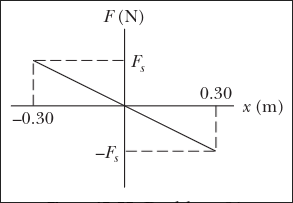
\includegraphics[width=0.45\linewidth]{images/81.png}
  \caption{Grafik gaya terhadap posisi (Gambar 15-55)}
\end{figure}}{}

\diketahui\ (nilai $x$ di ujung grafik dibaca dari Gambar 15-55)
\begin{align*}
m &= \SI{0,50}{\kilo\gram},&
F_s &= \SI{75,0}{\newton},&
x_s &= \SI{0,30}{\metre}.
\end{align*}
\ditanya\ (a) $x_m$; (b) $T$; (c) $a_{\max}$; (d) $K_{\max}$.

\konsep\ Gaya total pada GHS adalah gaya pegas, $|F| = k|x|$, sehingga grafik $|F|$ terhadap $x$ berupa garis lurus dengan kemiringan $k$. Gaya terbesar $F_s$ terjadi pada simpangan terjauh, yaitu amplitudo $x_m$.

\penyelesaian

\noindent\textbf{(a) Amplitudo}

Dari grafik, gaya mencapai $F_s$ pada $x_m = x_s = \SI{0,30}{\metre}$.

\noindent\textbf{(b) Periode}
\begin{align*}
k &= \frac{F_s}{x_m} = \frac{\SI{75,0}{\newton}}{\SI{0,30}{\metre}} = \SI{250}{\newton\per\metre},\\
T &= 2\pi\sqrt{\frac{m}{k}} = 2\pi\sqrt{\frac{\SI{0,50}{\kilo\gram}}{\SI{250}{\newton\per\metre}}}
= \SI{0,281}{\second}.
\end{align*}

\noindent\textbf{(c) Percepatan maksimum}
\begin{align*}
a_{\max} &= \frac{F_s}{m} = \frac{\SI{75,0}{\newton}}{\SI{0,50}{\kilo\gram}}
= \SI{150}{\metre\per\second\squared}.
\end{align*}

\noindent\textbf{(d) Energi kinetik maksimum}

Energi kinetik maksimum sama dengan energi mekanik total:
\begin{align*}
K_{\max} &= \frac12 k x_m^2 = \frac12 (\SI{250}{\newton\per\metre})(\SI{0,30}{\metre})^2
= \SI{11,25}{\joule}.
\end{align*}
\begin{jawaban}
(a) $x_m = \SI{0,30}{\metre}$ \quad (b) $T \approx \SI{0,281}{\second}$ \quad
(c) $a_{\max} = \SI{150}{\metre\per\second\squared}$ \quad
(d) $K_{\max} \approx \SI{11}{\joule}$.
\end{jawaban}

% ---------------------------------------------------------------------
\soal{89}
Sebuah partikel bermassa \SI{3,0}{\kilo\gram} bergerak harmonik sederhana satu dimensi menurut persamaan
\[
x=(\SI{5,0}{\metre})\cos\!\left[\left(\tfrac{\pi}{3}\,\si{\radian\per\second}\right)t-\tfrac{\pi}{4}\,\si{\radian}\right],
\]
dengan $t$ dalam sekon. (a) Pada nilai $x$ berapa energi potensial partikel sama dengan setengah energi totalnya? (b) Berapa lama partikel bergerak dari titik setimbang ke posisi $x$ tersebut?

\diketahui
\begin{align*}
m &= \SI{3,0}{\kilo\gram},&
x_m &= \SI{5,0}{\metre},&
\omega &= \frac{\pi}{3}\,\si{\radian\per\second}.
\end{align*}
\ditanya\ (a) $x$ saat $U=\tfrac12 E$; (b) selang waktu dari $x=0$ ke posisi tersebut.

\konsep\ Energi total $E=\tfrac12 k x_m^2$ dan energi potensial $U=\tfrac12 k x^2$. Pada GHS, fase $\omega t+\phi$ bertambah secara seragam terhadap waktu, sehingga selang waktu sama dengan selang fase dibagi $\omega$.

\penyelesaian

\noindent\textbf{(a) Posisi saat $U = E/2$}
\begin{align*}
\frac12 k x^2 &= \frac12\left(\frac12 k x_m^2\right)
\;\Rightarrow\; x = \pm\frac{x_m}{\sqrt2}\\
&= \pm\frac{\SI{5,0}{\metre}}{\sqrt2} = \pm\SI{3,5}{\metre}.
\end{align*}

\noindent\textbf{(b) Waktu dari titik setimbang}

Karena $x = x_m\cos\theta$ dengan $\theta=\omega t+\phi$, titik setimbang berada pada $\theta=\pi/2$ dan $x=x_m/\sqrt2$ pada $\theta=\pi/4$, sehingga selisih fasenya $\Delta\theta=\pi/4$:
\begin{align*}
\Delta t &= \frac{\Delta\theta}{\omega} = \frac{\pi/4}{\pi/3}\,\si{\second} = \SI{0,75}{\second}.
\end{align*}
\begin{jawaban}
(a) $x = \pm\SI{3,5}{\metre}$ \quad (b) $\Delta t = \SI{0,75}{\second}$.

Massa partikel tidak diperlukan karena yang ditanyakan hanya perbandingan energi dan waktu.
\end{jawaban}

% ---------------------------------------------------------------------
\soal{90}
Sebuah partikel melakukan GHS linear dengan frekuensi \SI{0,25}{\hertz} di sekitar titik $x=0$. Pada $t=0$ partikel memiliki simpangan $x=\SI{0,37}{\centi\metre}$ dan kecepatan nol. Tentukan (a) periode, (b) frekuensi sudut, (c) amplitudo, (d) simpangan $x(t)$, (e) kecepatan $v(t)$, (f) laju maksimum, (g) besar percepatan maksimum, (h) simpangan pada $t=\SI{3,0}{\second}$, dan (i) laju pada $t=\SI{3,0}{\second}$.

\diketahui
\begin{align*}
f &= \SI{0,25}{\hertz},&
x(0) &= \SI{0,37}{\centi\metre},&
v(0) &= 0.
\end{align*}
\ditanya\ (a) $T$; (b) $\omega$; (c) $x_m$; (d) $x(t)$; (e) $v(t)$; (f) $v_{\max}$; (g) $a_{\max}$; (h) $x(\SI{3,0}{\second})$; (i) $|v(\SI{3,0}{\second})|$.

\konsep\ GHS dinyatakan oleh $x=x_m\cos(\omega t+\phi)$ dengan $v=-\omega x_m\sin(\omega t+\phi)$. Karena $v(0)=0$, partikel berada di simpangan terjauhnya pada $t=0$, sehingga $x_m=x(0)$ dan $\phi=0$.

\penyelesaian

\noindent\textbf{(a), (b), (c)}
\begin{align*}
T &= \frac1f = \frac{1}{\SI{0,25}{\hertz}} = \SI{4,0}{\second},\\
\omega &= 2\pi f = 2\pi(\SI{0,25}{\hertz}) = \SI{1,57}{\radian\per\second}
\;\left(=\tfrac{\pi}{2}\,\si{\radian\per\second}\right),\\
x_m &= x(0) = \SI{0,37}{\centi\metre}.
\end{align*}

\noindent\textbf{(d), (e) Persamaan gerak}
\begin{align*}
x(t) &= (\SI{0,37}{\centi\metre})\cos\!\big[(\SI{1,57}{\radian\per\second})\,t\big],\\
v(t) &= -\omega x_m\sin\omega t
= -(\SI{0,58}{\centi\metre\per\second})\sin\!\big[(\SI{1,57}{\radian\per\second})\,t\big].
\end{align*}

\noindent\textbf{(f), (g) Nilai maksimum}
\begin{align*}
v_{\max} &= \omega x_m = (\SI{1,57}{\per\second})(\SI{0,37}{\centi\metre}) = \SI{0,58}{\centi\metre\per\second},\\
a_{\max} &= \omega^2 x_m = (\SI{1,57}{\per\second})^2(\SI{0,37}{\centi\metre}) = \SI{0,91}{\centi\metre\per\second\squared}.
\end{align*}

\noindent\textbf{(h), (i) Pada $t=\SI{3,0}{\second}$}

Fasenya $\omega t = \tfrac{\pi}{2}(3{,}0)=\tfrac{3\pi}{2}\,\si{\radian}$, sehingga
\begin{align*}
x(\SI{3,0}{\second}) &= (\SI{0,37}{\centi\metre})\cos\frac{3\pi}{2} = 0,\\
|v(\SI{3,0}{\second})| &= (\SI{0,58}{\centi\metre\per\second})\left|\sin\frac{3\pi}{2}\right| = \SI{0,58}{\centi\metre\per\second}.
\end{align*}
\begin{jawaban}
(a) $\SI{4,0}{\second}$ \quad (b) $\SI{1,57}{\radian\per\second}$ \quad (c) $\SI{0,37}{\centi\metre}$ \\
(d) $x=(\SI{0,37}{\centi\metre})\cos(\SI{1,57}{\radian\per\second}\,t)$ \\
(e) $v=-(\SI{0,58}{\centi\metre\per\second})\sin(\SI{1,57}{\radian\per\second}\,t)$ \\
(f) $\SI{0,58}{\centi\metre\per\second}$ \quad (g) $\SI{0,91}{\centi\metre\per\second\squared}$ \\
(h) $0$ \quad (i) $\SI{0,58}{\centi\metre\per\second}$ (laju maksimum, karena partikel melewati titik setimbang).
\end{jawaban}

% ---------------------------------------------------------------------
\soal{91}
Berapakah frekuensi bandul sederhana sepanjang \SI{2,0}{\metre} (a) di dalam ruangan, (b) di dalam lift yang dipercepat ke atas dengan percepatan \SI{2,0}{\metre\per\second\squared}, dan (c) dalam jatuh bebas?

\diketahui
\begin{align*}
L &= \SI{2,0}{\metre},&
a &= \SI{2,0}{\metre\per\second\squared}\ (\text{lift ke atas}).
\end{align*}
\ditanya\ Frekuensi $f$ pada (a) ruangan diam, (b) lift dipercepat ke atas, (c) jatuh bebas.

\konsep\ Frekuensi bandul sederhana $f=\dfrac{1}{2\pi}\sqrt{g_{\mathrm{ef}}/L}$. Di dalam kerangka yang dipercepat, $g$ diganti percepatan gravitasi efektif $g_{\mathrm{ef}}$: $g+a$ untuk percepatan ke atas, dan $g-g=0$ untuk jatuh bebas.

\penyelesaian

\noindent\textbf{(a) Dalam ruangan}
\begin{align*}
f &= \frac{1}{2\pi}\sqrt{\frac{g}{L}}
= \frac{1}{2\pi}\sqrt{\frac{\SI{9,8}{\metre\per\second\squared}}{\SI{2,0}{\metre}}}
= \SI{0,35}{\hertz}.
\end{align*}

\noindent\textbf{(b) Lift dipercepat ke atas}
\begin{align*}
g_{\mathrm{ef}} &= g + a = \SI{9,8}{\metre\per\second\squared} + \SI{2,0}{\metre\per\second\squared} = \SI{11,8}{\metre\per\second\squared},\\
f &= \frac{1}{2\pi}\sqrt{\frac{\SI{11,8}{\metre\per\second\squared}}{\SI{2,0}{\metre}}} = \SI{0,39}{\hertz}.
\end{align*}

\noindent\textbf{(c) Jatuh bebas}

Percepatan kerangka sama dengan $g$ ke bawah, sehingga $g_{\mathrm{ef}}=0$ dan $f=0$.
\begin{jawaban}
(a) $\SI{0,35}{\hertz}$ \quad (b) $\SI{0,39}{\hertz}$ \quad (c) $0$ (bandul tidak berosilasi).
\end{jawaban}

% ---------------------------------------------------------------------
\soal{92}
Sebuah jam kakek memiliki bandul berupa cakram kuningan tipis berjari-jari $r=\SI{15,00}{\centi\metre}$ dan bermassa \SI{1,000}{\kilo\gram} yang dipasang pada batang panjang tipis bermassa dapat diabaikan. Bandul berayun bebas pada sumbu yang tegak lurus batang dan melalui ujung batang yang berlawanan dengan cakram (Gambar 15-56). Jika bandul harus berperiode \SI{2,000}{\second} untuk osilasi kecil di tempat dengan $g=\SI{9,800}{\metre\per\second\squared}$, berapa panjang batang $L$ (dalam persepuluh milimeter terdekat)?

\IfFileExists{images/92.png}{%
\begin{figure}[H]
  \centering
  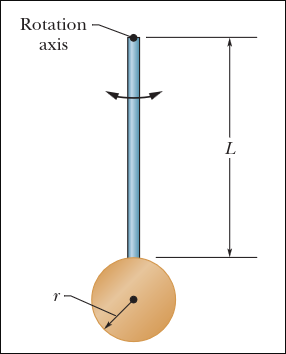
\includegraphics[width=0.3\linewidth]{images/92.png}
  \caption{Bandul jam kakek (Gambar 15-56)}
\end{figure}}{}

\diketahui
\begin{align*}
r &= \SI{0,1500}{\metre},&
m &= \SI{1,000}{\kilo\gram},&
T &= \SI{2,000}{\second},&
g &= \SI{9,800}{\metre\per\second\squared}.
\end{align*}
\ditanya\ Panjang batang $L$.

\konsep\ Bandul ini adalah bandul fisis dengan $T=2\pi\sqrt{I/(mgh)}$, dengan $h$ jarak titik tumpu ke pusat massa, yaitu pusat cakram: $h=L+r$ (massa batang diabaikan). Momen inersia cakram terhadap titik tumpu diperoleh dari teorema sumbu sejajar: $I=\tfrac12 mr^2+mh^2$.

\penyelesaian

Dari rumus periode,
\begin{align*}
\frac{T^2}{4\pi^2} &= \frac{\tfrac12 r^2 + h^2}{g\,h}
\;\Rightarrow\;
h^2 - \frac{gT^2}{4\pi^2}\,h + \frac{r^2}{2} = 0.
\end{align*}
Dengan
\begin{align*}
\frac{gT^2}{4\pi^2} &= \frac{(\SI{9,800}{\metre\per\second\squared})(\SI{2,000}{\second})^2}{4\pi^2} = \SI{0,99295}{\metre},\qquad
\frac{r^2}{2} = \SI{0,01125}{\metre\squared},
\end{align*}
persamaan kuadrat memberi
\begin{align*}
h &= \frac{0{,}99295 \pm \sqrt{(0{,}99295)^2 - 4(0{,}01125)}}{2}\,\si{\metre}
= \frac{0{,}99295 \pm 0{,}97003}{2}\,\si{\metre}.
\end{align*}
Akar yang lebih kecil ($h=\SI{0,0115}{\metre}$) tidak mungkin karena $h\ge r$, sehingga $h=\SI{0,98149}{\metre}$. Maka
\begin{align*}
L &= h - r = \SI{0,98149}{\metre} - \SI{0,1500}{\metre} = \SI{0,8315}{\metre}.
\end{align*}
\begin{jawaban}
\[
\boxed{L \approx \SI{0,8315}{\metre} = \SI{831,5}{\milli\metre}}
\]
\end{jawaban}

% ---------------------------------------------------------------------
\soal{109}
Bandul fisis pada Gambar 15-62 memiliki dua titik tumpu yang mungkin, A dan B. Titik A berposisi tetap, sedangkan B dapat digeser sepanjang bandul sesuai skala pada gambar. Bila digantung pada A, bandul berperiode $T=\SI{1,80}{\second}$. Bandul kemudian digantung pada B, yang digeser hingga bandul kembali berperiode sama. Berapa jarak $L$ antara A dan B?

\IfFileExists{images/109.png}{%
\begin{figure}[H]
  \centering
  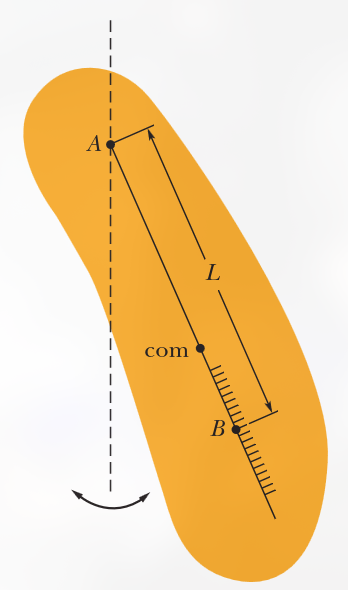
\includegraphics[width=0.3\linewidth]{images/109.png}
  \caption{Bandul fisis dengan titik tumpu A dan B (Gambar 15-62)}
\end{figure}}{}

\diketahui
\begin{align*}
T &= \SI{1,80}{\second},&
g &= \SI{9,8}{\metre\per\second\squared}.
\end{align*}
\ditanya\ Jarak $L = AB$.

\konsep\ Bandul fisis yang digantung pada A berperiode $T=2\pi\sqrt{I_A/(mgh_A)}$, yaitu sama dengan bandul sederhana sepanjang $L_0=\dfrac{I_A}{mh_A}$ ($h_A$ jarak A ke pusat massa). Titik B yang memberi periode sama berada pada garis A--pusat massa, di seberang pusat massa, pada jarak $L_0$ dari A (titik-titik sekawan, seperti pada bandul Kater).

\penyelesaian

\noindent\textbf{Pembuktian jarak AB $=L_0$}

Misalkan $h_B$ jarak B ke pusat massa. Karena $I_A = I_{\mathrm{pm}} + mh_A^2 = mh_AL_0$, diperoleh $I_{\mathrm{pm}} = mh_A(L_0-h_A)$. Bila $h_B = L_0 - h_A$, maka
\begin{align*}
\frac{I_B}{mh_B} &= \frac{I_{\mathrm{pm}}+mh_B^2}{mh_B}
= \frac{mh_Ah_B + mh_B^2}{mh_B} = h_A+h_B = L_0,
\end{align*}
sehingga periode di B sama dengan di A dan $AB = h_A+h_B = L_0$.

\noindent\textbf{Perhitungan}
\begin{align*}
T &= 2\pi\sqrt{\frac{L}{g}}
\;\Rightarrow\;
L = \frac{gT^2}{4\pi^2}
= \frac{(\SI{9,8}{\metre\per\second\squared})(\SI{1,80}{\second})^2}{4\pi^2}
= \SI{0,804}{\metre}.
\end{align*}
\begin{jawaban}
\[
\boxed{L \approx \SI{0,804}{\metre}}
\]
\end{jawaban}

% ---------------------------------------------------------------------
\soal{111}
Sebuah balok \SI{2,0}{\kilo\gram} melakukan GHS pada pegas horizontal dengan konstanta \SI{200}{\newton\per\metre}. Laju maksimum balok saat meluncur pada permukaan datar tanpa gesekan adalah \SI{3,0}{\metre\per\second}. Tentukan (a) amplitudo gerak balok, (b) besar percepatan maksimum, (c) besar percepatan minimum, dan (d) waktu yang diperlukan balok untuk menyelesaikan \num{7,0} siklus.

\diketahui
\begin{align*}
m &= \SI{2,0}{\kilo\gram},&
k &= \SI{200}{\newton\per\metre},&
v_{\max} &= \SI{3,0}{\metre\per\second}.
\end{align*}
\ditanya\ (a) $x_m$; (b) $a_{\max}$; (c) $a_{\min}$; (d) waktu untuk 7 siklus.

\konsep\ $\omega=\sqrt{k/m}$, $v_{\max}=\omega x_m$, $a_{\max}=\omega^2x_m$, dan $T=2\pi/\omega$. Percepatan $a=-\omega^2x$ bernilai nol di titik setimbang.

\penyelesaian

\noindent\textbf{(a) Amplitudo}
\begin{align*}
\omega &= \sqrt{\frac{k}{m}} = \sqrt{\frac{\SI{200}{\newton\per\metre}}{\SI{2,0}{\kilo\gram}}} = \SI{10}{\radian\per\second},\\
x_m &= \frac{v_{\max}}{\omega} = \frac{\SI{3,0}{\metre\per\second}}{\SI{10}{\per\second}} = \SI{0,30}{\metre}.
\end{align*}

\noindent\textbf{(b) Percepatan maksimum}
\begin{align*}
a_{\max} &= \omega^2 x_m = (\SI{10}{\per\second})^2(\SI{0,30}{\metre}) = \SI{30}{\metre\per\second\squared}.
\end{align*}

\noindent\textbf{(c) Percepatan minimum}

Besar percepatan terkecil terjadi di titik setimbang ($x=0$): $a_{\min}=0$.

\noindent\textbf{(d) Waktu untuk 7 siklus}
\begin{align*}
T &= \frac{2\pi}{\omega} = \frac{2\pi}{\SI{10}{\per\second}} = \SI{0,628}{\second},\\
t &= 7T = 7(\SI{0,628}{\second}) = \SI{4,4}{\second}.
\end{align*}
\begin{jawaban}
(a) $\SI{0,30}{\metre}$ \quad (b) $\SI{30}{\metre\per\second\squared}$ \quad (c) $0$ \quad (d) $\SI{4,4}{\second}$.
\end{jawaban}

% ---------------------------------------------------------------------
\soal{112}
Pada Gambar 15-64, bola penghancur bermassa \SI{2500}{\kilo\gram} berayun dari ujung sebuah derek. Panjang bagian kabel yang berayun adalah \SI{17}{\metre}. (a) Tentukan periode ayunan dengan menganggap sistem sebagai bandul sederhana. (b) Apakah periode bergantung pada massa bola?

\diketahui
\begin{align*}
m &= \SI{2500}{\kilo\gram},&
L &= \SI{17}{\metre}.
\end{align*}
\ditanya\ (a) Periode $T$; (b) apakah $T$ bergantung pada $m$.

\konsep\ Periode bandul sederhana untuk osilasi kecil: $T=2\pi\sqrt{L/g}$.

\penyelesaian

\noindent\textbf{(a) Periode}
\begin{align*}
T &= 2\pi\sqrt{\frac{L}{g}} = 2\pi\sqrt{\frac{\SI{17}{\metre}}{\SI{9,8}{\metre\per\second\squared}}}
= \SI{8,3}{\second}.
\end{align*}

\noindent\textbf{(b) Pengaruh massa}

Massa $m$ tidak muncul dalam rumus $T=2\pi\sqrt{L/g}$ (gaya pemulih $mg\sin\theta$ sebanding dengan massa, demikian pula kelembaman $mL^2$, sehingga massa saling meniadakan). Jadi periode tidak bergantung pada massa bola.
\begin{jawaban}
(a) $T \approx \SI{8,3}{\second}$ \quad (b) Tidak, periode tidak bergantung pada massa.
\end{jawaban}

% ---------------------------------------------------------------------
\soal{114}
Sebuah ketapel besar (hipotetis) ditarik sejauh \SI{2,30}{\metre} untuk meluncurkan proyektil \SI{170}{\gram} dengan laju yang cukup untuk lepas dari Bumi (\SI{11,2}{\kilo\metre\per\second}). Anggap karet ketapel memenuhi hukum Hooke. (a) Berapakah konstanta pegas alat ini jika seluruh energi potensial elastik berubah menjadi energi kinetik? (b) Anggap seseorang rata-rata dapat mengerahkan gaya \SI{490}{\newton}. Berapa orang yang dibutuhkan untuk menarik karet tersebut?

\diketahui
\begin{align*}
x &= \SI{2,30}{\metre},&
m &= \SI{0,170}{\kilo\gram},&
v &= \SI{1,12e4}{\metre\per\second},&
F_{\text{orang}} &= \SI{490}{\newton}.
\end{align*}
\ditanya\ (a) Konstanta pegas $k$; (b) jumlah orang $N$.

\konsep\ Kekekalan energi: $\tfrac12kx^2=\tfrac12mv^2$. Gaya tarik pada simpangan $x$ adalah $F=kx$ (hukum Hooke), dan jumlah orang adalah $N=F/F_{\text{orang}}$.

\penyelesaian

\noindent\textbf{(a) Konstanta pegas}
\begin{align*}
k &= \frac{mv^2}{x^2}
= \frac{(\SI{0,170}{\kilo\gram})(\SI{1,12e4}{\metre\per\second})^2}{(\SI{2,30}{\metre})^2}
= \SI{4,03e6}{\newton\per\metre}.
\end{align*}

\noindent\textbf{(b) Jumlah orang}
\begin{align*}
F &= kx = (\SI{4,03e6}{\newton\per\metre})(\SI{2,30}{\metre}) = \SI{9,27e6}{\newton},\\
N &= \frac{F}{F_{\text{orang}}} = \frac{\SI{9,27e6}{\newton}}{\SI{490}{\newton}} \approx \num{1,9e4}.
\end{align*}
\begin{jawaban}
(a) $k \approx \SI{4,03e6}{\newton\per\metre}$ \quad
(b) sekitar $\num{1,9e4}$ orang (sekitar \num{18922}, dibulatkan ke atas menjadi \num{18923} orang).
\end{jawaban}

% ---------------------------------------------------------------------
\soal{115}
Berapakah panjang bandul sederhana yang satu ayunan penuh dari kiri ke kanan lalu kembali lagi memerlukan waktu \SI{3,2}{\second}?

\diketahui
\begin{align*}
T &= \SI{3,2}{\second}\ (\text{satu ayunan penuh}),&
g &= \SI{9,8}{\metre\per\second\squared}.
\end{align*}
\ditanya\ Panjang bandul $L$.

\konsep\ Satu ayunan penuh (kiri ke kanan lalu kembali) adalah satu periode, sehingga $T=2\pi\sqrt{L/g}$.

\penyelesaian
\begin{align*}
L &= \frac{gT^2}{4\pi^2}
= \frac{(\SI{9,8}{\metre\per\second\squared})(\SI{3,2}{\second})^2}{4\pi^2}
= \SI{2,5}{\metre}.
\end{align*}
\begin{jawaban}
\[
\boxed{L \approx \SI{2,5}{\metre}}
\]
\end{jawaban}

% =====================================================================
% BAB 16 -- GELOMBANG I   (potongan untuk ditempel ke main.tex)
% Memakai makro yang sudah ada di main.tex: \bab, \soal, rumusutama,
% \diketahui, \ditanya, \konsep, \penyelesaian, jawaban.
% =====================================================================
\bab{16}{Gelombang I}

\begin{rumusutama}
\begin{itemize}[nosep,leftmargin=*]
  \item \textbf{Gelombang sinusoidal:}
        $y(x,t) = y_m\sin(kx - \omega t + \phi)$, \quad
        $k = \dfrac{2\pi}{\lambda}$, \quad $\omega = 2\pi f = \dfrac{2\pi}{T}$
  \item \textbf{Laju gelombang:}
        $v = \dfrac{\omega}{k} = \lambda f$; \quad pada tali
        $v = \sqrt{\dfrac{\tau}{\mu}}$
  \item \textbf{Kecepatan transversal partikel:}
        $u = \dfrac{\partial y}{\partial t}$, \quad $u_{\max} = \omega y_m$
  \item \textbf{Persamaan gelombang:}
        $\dfrac{\partial^2 y}{\partial x^2} = \dfrac{1}{v^2}\dfrac{\partial^2 y}{\partial t^2}$
  \item \textbf{Daya rata-rata pada tali:}
        $P_{\text{rata}} = \tfrac{1}{2}\mu v\,\omega^2 y_m^2$
  \item \textbf{Interferensi dua gelombang} (beda fase $\phi$):
        $y_m' = \sqrt{y_{m1}^2 + y_{m2}^2 + 2y_{m1}y_{m2}\cos\phi}$ \quad
        (sama amplitudo: $y_m' = 2y_m\cos\tfrac{\phi}{2}$)
  \item \textbf{Gelombang berdiri:}
        $y'(x,t) = \left[2y_m\sin kx\right]\cos\omega t$, \quad
        $f = \dfrac{nv}{2L}$ \; ($n = 1,2,3,\dots$)
\end{itemize}
\par\smallskip\noindent\footnotesize Rumus mengacu pada \cite{halliday}.
\end{rumusutama}

% ---------------------------------------------------------------------
\soal{2}
\textit{Gelombang manusia.} Pada pertandingan olahraga di stadion yang padat, penonton membuat gelombang (pulsa) yang bergerak mengelilingi stadion. Saat gelombang tiba, sekelompok penonton berdiri sambil bersorak lalu duduk lagi. Pada suatu saat, lebar $w$ gelombang adalah jarak dari tepi depan (orang yang hampir berdiri) sampai tepi belakang (orang yang baru saja duduk). Misalkan gelombang manusia menempuh \num{853} kursi mengelilingi stadion dalam \SI{39}{\second}, dan penonton memerlukan sekitar \SI{1,8}{\second} untuk berdiri lalu duduk. Berapa (a) laju gelombang $v$ (kursi per sekon) dan (b) lebar $w$ (dalam jumlah kursi)?

\diketahui
\begin{align*}
	d        & = \num{853}\ \text{kursi}, &
	t        & = \SI{39}{\second},        &
	\Delta t & = \SI{1,8}{\second}.
\end{align*}
\ditanya\ (a) $v$; (b) $w$.

\konsep\ Laju gelombang adalah jarak tempuh dibagi waktu tempuh. Lebar gelombang adalah jarak yang ditempuh gelombang selama satu kelompok penonton berdiri lalu duduk: $w=v\,\Delta t$.

\penyelesaian

\noindent\textbf{(a) Laju gelombang}
\begin{align*}
	v & = \frac{d}{t} = \frac{\num{853}\ \text{kursi}}{\SI{39}{\second}} = \SI{21,9}{\text{kursi}\per\second}\approx \SI{22}{\text{kursi}\per\second}.
\end{align*}

\noindent\textbf{(b) Lebar gelombang}
\begin{align*}
	w & = v\,\Delta t = (\SI{21,87}{\text{kursi}\per\second})(\SI{1,8}{\second}) = \num{39,4}\ \text{kursi}\approx 39\ \text{kursi}.
\end{align*}
\begin{jawaban}
	(a) $v \approx \SI{22}{\text{kursi}\per\second}$ \quad (b) $w \approx 39$ kursi.
\end{jawaban}

% ---------------------------------------------------------------------
\soal{3}
Sebuah gelombang memiliki frekuensi sudut \SI{110}{\radian\per\second} dan panjang gelombang \SI{1,80}{\metre}. Hitung (a) bilangan gelombang sudut dan (b) laju gelombang.

\diketahui
\begin{align*}
	\omega  & = \SI{110}{\radian\per\second}, &
	\lambda & = \SI{1,80}{\metre}.
\end{align*}
\ditanya\ (a) $k$; (b) $v$.

\konsep\ $k=\dfrac{2\pi}{\lambda}$ dan $v=\dfrac{\omega}{k}$.

\penyelesaian

\noindent\textbf{(a) Bilangan gelombang sudut}
\begin{align*}
	k & = \frac{2\pi}{\lambda} = \frac{2\pi}{\SI{1,80}{\metre}} = \SI{3,49}{\radian\per\metre}.
\end{align*}

\noindent\textbf{(b) Laju gelombang}
\begin{align*}
	v & = \frac{\omega}{k} = \frac{\SI{110}{\radian\per\second}}{\SI{3,49}{\radian\per\metre}} = \SI{31,5}{\metre\per\second}.
\end{align*}
\begin{jawaban}
	(a) $k \approx \SI{3,49}{\radian\per\metre}$ \quad (b) $v \approx \SI{31,5}{\metre\per\second}$.
\end{jawaban}

% ---------------------------------------------------------------------
\soal{6}
Sebuah gelombang sinusoidal merambat sepanjang tali yang tegang. Gambar 16-31 menunjukkan kemiringan (gradien) tali sepanjang sumbu $x$ pada $t=0$. Skala sumbu $x$ ditetapkan oleh $x_s=\SI{0,80}{\metre}$. Berapakah amplitudo gelombang?

\IfFileExists{images/6.png}{%
	\begin{figure}[H]
		\centering
		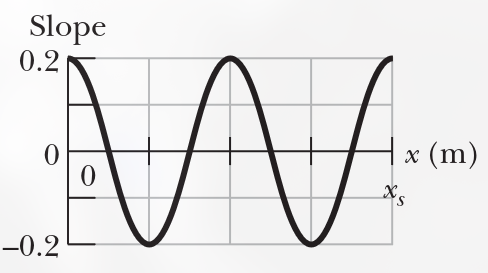
\includegraphics[width=0.45\linewidth]{images/6.png}
		\caption{Kemiringan tali pada $t=0$ (Gambar 16-31)}
	\end{figure}}{}

\diketahui\ (dibaca dari Gambar 16-31: $x_s$ memuat dua panjang gelombang, dan kemiringan maksimum tali bernilai \num{0,20})
\begin{align*}
	x_s                                               & = 2\lambda = \SI{0,80}{\metre}, &
	\left(\frac{\partial y}{\partial x}\right)_{\max} & = \num{0,20}.
\end{align*}
\ditanya\ Amplitudo $y_m$.

\konsep\ Untuk $y=y_m\sin(kx-\omega t+\phi)$, kemiringan tali adalah $\dfrac{\partial y}{\partial x}=y_m k\cos(kx-\omega t+\phi)$, sehingga kemiringan maksimumnya $y_m k$.

\penyelesaian
\begin{align*}
	\lambda & = \frac{x_s}{2} = \SI{0,40}{\metre},\qquad
	k = \frac{2\pi}{\lambda} = \frac{2\pi}{\SI{0,40}{\metre}} = \SI{15,7}{\radian\per\metre}, \\
	y_m k   & = 0{,}20
	\;\Rightarrow\;
	y_m = \frac{0{,}20}{\SI{15,7}{\per\metre}} = \SI{0,0127}{\metre}.
\end{align*}
\begin{jawaban}
	\[
		\boxed{y_m \approx \SI{1,3}{\centi\metre}}
	\]
	Catatan: \num{0,20} adalah kemiringan maksimum yang dibaca dari grafik (tanpa satuan), bukan amplitudo.
\end{jawaban}

% ---------------------------------------------------------------------
\soal{8}
Gambar 16-32 menunjukkan kecepatan transversal $u$ terhadap waktu $t$ untuk titik pada tali di $x=0$ saat sebuah gelombang melewatinya. Skala sumbu vertikal ditetapkan oleh $u_s=\SI{4,0}{\metre\per\second}$. Gelombang berbentuk umum $y(x,t)=y_m\sin(kx-\omega t+\phi)$. Berapakah $\phi$?

\IfFileExists{images/8.png}{%
	\begin{figure}[H]
		\centering
		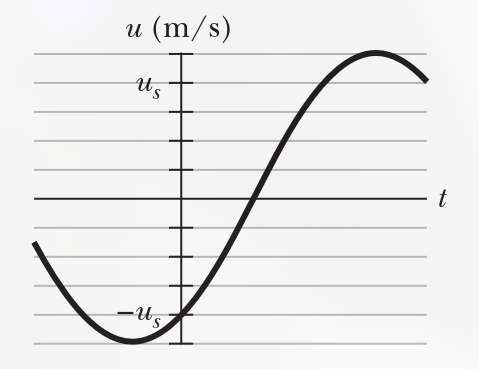
\includegraphics[width=0.45\linewidth]{images/8.png}
		\caption{Kecepatan transversal terhadap waktu di $x=0$ (Gambar 16-32)}
	\end{figure}}{}

\diketahui\ (dibaca dari Gambar 16-32: pada $t=0$ kecepatan transversal $u=-u_s$ dan sedang naik; nilai maksimum kurva $u_{\max}=\SI{5,0}{\metre\per\second}$)
\begin{align*}
	u(0)     & = -\SI{4,0}{\metre\per\second},           &
	u_{\max} & = \omega y_m=\SI{5,0}{\metre\per\second}.
\end{align*}
\ditanya\ Konstanta fase $\phi$.

\konsep\ Di $x=0$, $y=y_m\sin(\phi-\omega t)$, sehingga $u=\dfrac{\partial y}{\partial t}=-\omega y_m\cos(\phi-\omega t)$ dan percepatan transversal $a_y=-\omega^2y_m\sin(\phi-\omega t)$. Nilai $\cos\phi$ ditentukan dari $u(0)$, sedangkan tanda $\phi$ ditentukan dari arah perubahan $u$ pada $t=0$.

\penyelesaian

Pada $t=0$:
\begin{align*}
	u(0) & = -\omega y_m\cos\phi = -(\SI{5,0}{\metre\per\second})\cos\phi = -\SI{4,0}{\metre\per\second}
	\;\Rightarrow\;
	\cos\phi = 0{,}80,                                                                                   \\
	\phi & = \pm\cos^{-1}(0{,}80) = \pm 0{,}6435\ \si{\radian}.
\end{align*}
Pada grafik, $u$ sedang naik di $t=0$, sehingga $a_y(0)>0$:
\begin{align*}
	a_y(0) & = -\omega^2 y_m\sin\phi > 0 \;\Rightarrow\; \sin\phi<0 \;\Rightarrow\; \phi = -0{,}6435\ \si{\radian}.
\end{align*}
\begin{jawaban}
	\[
		\boxed{\phi \approx -0{,}64\ \si{\radian}}\quad(\text{atau } 5{,}64\ \si{\radian}\ \text{karena } \phi\ \text{berulang tiap } 2\pi).
	\]
	Kalkulator hanya memberi $\cos^{-1}(0{,}80)=+0{,}6435$ \si{\radian}; tanda yang benar diperoleh dari arah perubahan $u$ pada grafik.
\end{jawaban}

% ---------------------------------------------------------------------
\soal{11}
Gelombang transversal sinusoidal dengan panjang gelombang \SI{20}{\centi\metre} merambat sepanjang tali ke arah $x$ positif. Simpangan $y$ partikel tali di $x=0$ diberikan pada Gambar 16-34 sebagai fungsi waktu $t$; skala sumbu vertikal ditetapkan oleh $y_s=\SI{4,0}{\centi\metre}$. Persamaan gelombang berbentuk $y(x,t)=y_m\sin(kx\pm\omega t+\phi)$. (a) Pada $t=0$, apakah grafik $y$ terhadap $x$ berbentuk fungsi sinus positif atau negatif? Tentukan (b) $y_m$, (c) $k$, (d) $\omega$, (e) $\phi$, (f) tanda di depan $\omega$, dan (g) laju gelombang. (h) Berapa kecepatan transversal partikel di $x=0$ pada $t=\SI{5,0}{\second}$?

\IfFileExists{images/11.png}{%
	\begin{figure}[H]
		\centering
		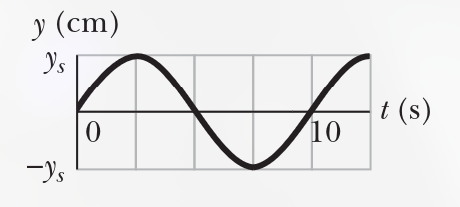
\includegraphics[width=0.45\linewidth]{images/11.png}
		\caption{Simpangan di $x=0$ terhadap waktu (Gambar 16-34)}
	\end{figure}}{}

\diketahui\ (dibaca dari Gambar 16-34: di $x=0$, $y(0,t)=+y_s\sin(2\pi t/T)$ dengan periode $T=\SI{10}{\second}$)
\begin{align*}
	\lambda & = \SI{20}{\centi\metre},  &
	y_s     & = \SI{4,0}{\centi\metre}, &
	T       & = \SI{10}{\second}.
\end{align*}
\ditanya\ (a) bentuk $y(x,0)$; (b) $y_m$; (c) $k$; (d) $\omega$; (e) $\phi$; (f) tanda $\omega$; (g) $v$; (h) $u(0,\SI{5,0}{\second})$.

\konsep\ Gelombang yang merambat ke $+x$ berbentuk $y=y_m\sin(kx-\omega t+\phi)$. Di $x=0$, $y(0,t)=y_m\sin(\phi-\omega t)$ harus sama dengan $+y_m\sin\omega t$, sehingga $\phi=\pi$ karena $\sin(\pi-\omega t)=\sin\omega t$.

\penyelesaian

\noindent\textbf{(a) Bentuk grafik $y(x,0)$}
\begin{align*}
	y(x,0) & = y_m\sin(kx+\pi) = -y_m\sin kx,
\end{align*}
yaitu fungsi \textbf{sinus negatif}.

\noindent\textbf{(b)--(f) Parameter gelombang}
\begin{align*}
	y_m    & = \SI{4,0}{\centi\metre},                                                                                                        \\
	k      & = \frac{2\pi}{\lambda} = \frac{2\pi}{\SI{20}{\centi\metre}} = \SI{0,31}{\radian\per\centi\metre}\;(=\SI{31}{\radian\per\metre}), \\
	\omega & = \frac{2\pi}{T} = \frac{2\pi}{\SI{10}{\second}} = \SI{0,63}{\radian\per\second},                                                \\
	\phi   & = \pi\ \si{\radian},\qquad \text{tanda di depan } \omega:\ \text{negatif } (kx-\omega t).
\end{align*}

\noindent\textbf{(g) Laju gelombang}
\begin{align*}
	v & = \frac{\omega}{k} = \frac{\SI{0,628}{\radian\per\second}}{\SI{0,314}{\radian\per\centi\metre}} = \SI{2,0}{\centi\metre\per\second}.
\end{align*}

\noindent\textbf{(h) Kecepatan transversal di $x=0$}

Di $x=0$, $y(0,t)=(\SI{4,0}{\centi\metre})\sin\omega t$, sehingga
\begin{align*}
	u(0,t)                 & = \frac{\partial y}{\partial t} = \omega y_m\cos\omega t,  \\
	u(0,\SI{5,0}{\second}) & = (\SI{0,628}{\per\second})(\SI{4,0}{\centi\metre})\cos\pi
	= -\SI{2,5}{\centi\metre\per\second}.
\end{align*}
\begin{jawaban}
	(a) sinus negatif \quad (b) $\SI{4,0}{\centi\metre}$ \quad (c) $\SI{0,31}{\radian\per\centi\metre}$ \quad
	(d) $\SI{0,63}{\radian\per\second}$ \quad (e) $\pi$ \si{\radian} \quad (f) negatif \quad
	(g) $\SI{2,0}{\centi\metre\per\second}$ \quad (h) $-\SI{2,5}{\centi\metre\per\second}$
	(bergerak ke bawah).
\end{jawaban}

% ---------------------------------------------------------------------
\soal{17}
Massa per satuan panjang sebuah tali adalah \SI{1,6e-4}{\kilo\gram\per\metre}. Gelombang transversal pada tali dinyatakan oleh persamaan
\[
	y=(\SI{0,021}{\metre})\sin\!\left[(\SI{2,0}{\per\metre})x+(\SI{30}{\per\second})t\right].
\]
Tentukan (a) laju gelombang dan (b) tegangan tali.

\diketahui
\begin{align*}
	\mu    & = \SI{1,6e-4}{\kilo\gram\per\metre}, &
	k      & = \SI{2,0}{\per\metre},              &
	\omega & = \SI{30}{\per\second}.
\end{align*}
\ditanya\ (a) $v$; (b) $\tau$.

\konsep\ Dengan membandingkan persamaan di atas dengan $y=y_m\sin(kx+\omega t)$, laju gelombang adalah $v=\omega/k$ (merambat ke arah $-x$). Untuk gelombang pada tali, $v=\sqrt{\tau/\mu}$ sehingga $\tau=\mu v^2$.

\penyelesaian

\noindent\textbf{(a) Laju gelombang}
\begin{align*}
	v & = \frac{\omega}{k} = \frac{\SI{30}{\per\second}}{\SI{2,0}{\per\metre}} = \SI{15}{\metre\per\second}.
\end{align*}

\noindent\textbf{(b) Tegangan tali}
\begin{align*}
	\tau & = \mu v^2 = (\SI{1,6e-4}{\kilo\gram\per\metre})(\SI{15}{\metre\per\second})^2 = \SI{0,036}{\newton}.
\end{align*}
\begin{jawaban}
	(a) $v = \SI{15}{\metre\per\second}$ \quad (b) $\tau = \SI{0,036}{\newton}$.
\end{jawaban}

% ---------------------------------------------------------------------
\soal{24}
Pada Gambar 16-36a, tali 1 memiliki massa per satuan panjang $\mu_1=\SI{3,00}{\gram\per\metre}$ dan tali 2 memiliki $\mu_2=\SI{5,00}{\gram\per\metre}$. Keduanya tegang akibat balok menggantung bermassa $M=\SI{500}{\gram}$. Hitung laju gelombang pada (a) tali 1 dan (b) tali 2. (\textit{Petunjuk:} bila tali melingkari katrol setengah putaran, tali menarik katrol dengan gaya total sebesar dua kali tegangan tali.) Selanjutnya balok dibagi menjadi dua balok ($M_1+M_2=M$) dan susunan diubah seperti Gambar 16-36b. Tentukan (c) $M_1$ dan (d) $M_2$ agar laju gelombang pada kedua tali sama.

\IfFileExists{images/24.png}{%
	\begin{figure}[H]
		\centering
		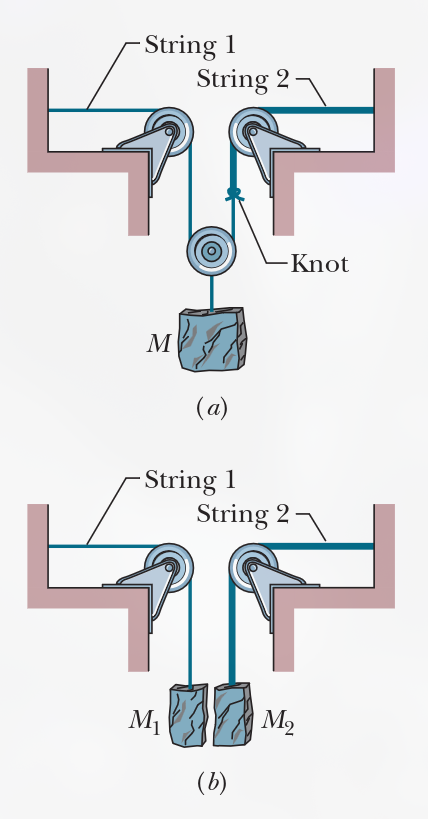
\includegraphics[width=0.6\linewidth]{images/24.png}
		\caption{Susunan tali dan balok (Gambar 16-36)}
	\end{figure}}{}

\diketahui
\begin{align*}
	\mu_1 & = \SI{3,00e-3}{\kilo\gram\per\metre}, &
	\mu_2 & = \SI{5,00e-3}{\kilo\gram\per\metre}, &
	M     & = \SI{0,500}{\kilo\gram}.
\end{align*}
\ditanya\ (a) $v_1$; (b) $v_2$; (c) $M_1$; (d) $M_2$.

\konsep\ $v=\sqrt{\tau/\mu}$. Pada susunan (a), tali melingkari katrol setengah putaran sehingga berat balok ditopang oleh dua bagian tali: $2\tau=Mg$, maka $\tau=Mg/2$ untuk kedua tali. Pada susunan (b), setiap tali ditegangkan oleh berat balok masing-masing: $\tau_1=M_1g$ dan $\tau_2=M_2g$.

\penyelesaian

\noindent\textbf{(a), (b) Laju gelombang}
\begin{align*}
	\tau & = \frac{Mg}{2} = \frac{(\SI{0,500}{\kilo\gram})(\SI{9,8}{\metre\per\second\squared})}{2} = \SI{2,45}{\newton},                     \\
	v_1  & = \sqrt{\frac{\tau}{\mu_1}} = \sqrt{\frac{\SI{2,45}{\newton}}{\SI{3,00e-3}{\kilo\gram\per\metre}}} = \SI{28,6}{\metre\per\second}, \\
	v_2  & = \sqrt{\frac{\tau}{\mu_2}} = \sqrt{\frac{\SI{2,45}{\newton}}{\SI{5,00e-3}{\kilo\gram\per\metre}}} = \SI{22,1}{\metre\per\second}.
\end{align*}

\noindent\textbf{(c), (d) Laju sama}
\begin{align*}
	\frac{M_1 g}{\mu_1} & = \frac{M_2 g}{\mu_2}
	\;\Rightarrow\; \frac{M_1}{M_2} = \frac{\mu_1}{\mu_2}=\frac{3}{5},\qquad M_1+M_2 = M,                                                         \\
	M_1                 & = \frac{\mu_1}{\mu_1+\mu_2}M = \frac{3{,}00}{8{,}00}(\SI{500}{\gram}) = \SI{187,5}{\gram}\approx\SI{0,188}{\kilo\gram}, \\
	M_2                 & = M - M_1 = \SI{312,5}{\gram}\approx\SI{0,313}{\kilo\gram}.
\end{align*}
\begin{jawaban}
	(a) $v_1 \approx \SI{28,6}{\metre\per\second}$ \quad (b) $v_2 \approx \SI{22,1}{\metre\per\second}$ \\
	(c) $M_1 \approx \SI{0,188}{\kilo\gram}$ \quad (d) $M_2 \approx \SI{0,313}{\kilo\gram}$.
\end{jawaban}

% ---------------------------------------------------------------------
\soal{26}
Sebuah tali sepanjang \SI{2,70}{\metre} dan bermassa \SI{260}{\gram} dapat dilalui gelombang. Tegangan tali \SI{36,0}{\newton}. Berapa frekuensi gelombang berjalan beramplitudo \SI{7,70}{\milli\metre} agar daya rata-ratanya \SI{85,0}{\watt}?

\diketahui
\begin{align*}
	L               & = \SI{2,70}{\metre},      &
	m               & = \SI{0,260}{\kilo\gram}, &
	\tau            & = \SI{36,0}{\newton},       \\
	y_m             & = \SI{7,70e-3}{\metre},   &
	P_{\text{rata}} & = \SI{85,0}{\watt}.
\end{align*}
\ditanya\ Frekuensi $f$.

\konsep\ $\mu=m/L$, $v=\sqrt{\tau/\mu}$, dan daya rata-rata $P_{\text{rata}}=\tfrac12\mu v\omega^2y_m^2$ dengan $\omega=2\pi f$.

\penyelesaian
\begin{align*}
	\mu    & = \frac{m}{L} = \frac{\SI{0,260}{\kilo\gram}}{\SI{2,70}{\metre}} = \SI{0,0963}{\kilo\gram\per\metre},                           \\
	v      & = \sqrt{\frac{\tau}{\mu}} = \sqrt{\frac{\SI{36,0}{\newton}}{\SI{0,0963}{\kilo\gram\per\metre}}} = \SI{19,3}{\metre\per\second}, \\
	\omega & = \sqrt{\frac{2P_{\text{rata}}}{\mu v y_m^2}}
	= \sqrt{\frac{2(\SI{85,0}{\watt})}{(\SI{0,0963}{\kilo\gram\per\metre})(\SI{19,3}{\metre\per\second})(\SI{7,70e-3}{\metre})^2}}
	= \SI{1,24e3}{\radian\per\second},                                                                                                       \\
	f      & = \frac{\omega}{2\pi} = \frac{\SI{1,24e3}{\radian\per\second}}{2\pi} = \SI{198}{\hertz}.
\end{align*}
\begin{jawaban}
	\[
		\boxed{f \approx \SI{198}{\hertz}}
	\]
\end{jawaban}

% ---------------------------------------------------------------------
\soal{28}
Gunakan persamaan gelombang untuk mencari laju gelombang yang dinyatakan oleh
\[
	y(x,t)=(\SI{3,00}{\milli\metre})\sin\!\left[(\SI{4,00}{\per\metre})x-(\SI{7,00}{\per\second})t\right].
\]

\diketahui
\begin{align*}
	y & = (\SI{3,00}{\milli\metre})\sin(4{,}00\,x-7{,}00\,t),\quad x\text{ dalam m},\ t\text{ dalam s}.
\end{align*}
\ditanya\ Laju gelombang $v$.

\konsep\ Persamaan gelombang: $\dfrac{\partial^2y}{\partial x^2}=\dfrac{1}{v^2}\dfrac{\partial^2y}{\partial t^2}$.

\penyelesaian
\begin{align*}
	\frac{\partial^2 y}{\partial x^2} & = -(4{,}00)^2\,y = -16{,}0\,y,\qquad
	\frac{\partial^2 y}{\partial t^2} = -(7{,}00)^2\,y = -49{,}0\,y,           \\
	-16{,}0\,y                        & = \frac{1}{v^2}\left(-49{,}0\,y\right)
	\;\Rightarrow\; v^2=\frac{49{,}0}{16{,}0}
	\;\Rightarrow\; v=\SI{1,75}{\metre\per\second}.
\end{align*}
\begin{jawaban}
	\[
		\boxed{v = \SI{1,75}{\metre\per\second}}\quad(\text{ke arah } +x).
	\]
\end{jawaban}

% ---------------------------------------------------------------------
\soal{29}
Gunakan persamaan gelombang untuk mencari laju gelombang yang dinyatakan oleh
\[
	y(x,t)=(\SI{2,00}{\milli\metre})\left[(\SI{20}{\per\metre})x-(\SI{4,0}{\per\second})t\right]^{0,5}.
\]

\diketahui
\begin{align*}
	y & = (\SI{2,00}{\milli\metre})\,\xi^{0,5},\qquad \xi = 20\,x-4{,}0\,t.
\end{align*}
\ditanya\ Laju gelombang $v$.

\konsep\ Gunakan persamaan gelombang $\dfrac{\partial^2y}{\partial x^2}=\dfrac{1}{v^2}\dfrac{\partial^2y}{\partial t^2}$. Fungsi tersebut bergantung pada $x$ dan $t$ hanya melalui $\xi=20x-4{,}0t$.

\penyelesaian

Dengan $y=A\xi^{1/2}$ dan aturan rantai ($\partial\xi/\partial x=20$, $\partial\xi/\partial t=-4{,}0$):
\begin{align*}
	\frac{\partial^2 y}{\partial x^2} & = (20)^2\,A\left(-\tfrac14\right)\xi^{-3/2} = -100\,A\,\xi^{-3/2},                          \\
	\frac{\partial^2 y}{\partial t^2} & = (4{,}0)^2\,A\left(-\tfrac14\right)\xi^{-3/2} = -4{,}0\,A\,\xi^{-3/2},                     \\
	v^2                               & = \frac{\partial^2 y/\partial t^2}{\partial^2 y/\partial x^2} = \frac{4{,}0}{100} = 0{,}040
	\;\Rightarrow\; v=\SI{0,20}{\metre\per\second}.
\end{align*}
\begin{jawaban}
	\[
		\boxed{v = \SI{0,20}{\metre\per\second}}\quad(\text{ke arah } +x,\ \text{sama dengan } 4{,}0/20).
	\]
\end{jawaban}

% ---------------------------------------------------------------------
\soal{30}
Gunakan persamaan gelombang untuk mencari laju gelombang yang dinyatakan dalam fungsi umum $h(x,t)$:
\[
	y(x,t)=(\SI{4,00}{\milli\metre})\,h\!\left[(\SI{30}{\per\metre})x+(\SI{6,0}{\per\second})t\right].
\]

\diketahui
\begin{align*}
	y & = (\SI{4,00}{\milli\metre})\,h(\xi),\qquad \xi = 30\,x+6{,}0\,t.
\end{align*}
\ditanya\ Laju gelombang $v$.

\konsep\ Gunakan persamaan gelombang dengan aturan rantai pada $h(\xi)$.

\penyelesaian
\begin{align*}
	\frac{\partial^2 y}{\partial x^2} & = (30)^2\,(\SI{4,00}{\milli\metre})\,h''(\xi) = 900\,(\SI{4,00}{\milli\metre})\,h'',   \\
	\frac{\partial^2 y}{\partial t^2} & = (6{,}0)^2\,(\SI{4,00}{\milli\metre})\,h''(\xi) = 36\,(\SI{4,00}{\milli\metre})\,h'', \\
	v^2                               & = \frac{36}{900} = 0{,}040
	\;\Rightarrow\; v=\SI{0,20}{\metre\per\second}.
\end{align*}
\begin{jawaban}
	\[
		\boxed{v = \SI{0,20}{\metre\per\second}}\quad(\text{ke arah } -x,\ \text{karena tanda } +\text{ pada } \xi).
	\]
\end{jawaban}

% ---------------------------------------------------------------------
\soal{36}
Empat gelombang dikirim sepanjang tali yang sama ke arah yang sama:
\begin{align*}
	y_1(x,t) & = (\SI{4,00}{\milli\metre})\sin(2\pi x-400\pi t),          \\
	y_2(x,t) & = (\SI{4,00}{\milli\metre})\sin(2\pi x-400\pi t+0{,}7\pi), \\
	y_3(x,t) & = (\SI{4,00}{\milli\metre})\sin(2\pi x-400\pi t+\pi),      \\
	y_4(x,t) & = (\SI{4,00}{\milli\metre})\sin(2\pi x-400\pi t+1{,}7\pi).
\end{align*}
Berapakah amplitudo gelombang resultan?

\diketahui
\begin{align*}
	y_{m1}=y_{m2}=y_{m3}=y_{m4} & = \SI{4,00}{\milli\metre},       &
	\phi_1,\phi_2,\phi_3,\phi_4 & = 0,\ 0{,}7\pi,\ \pi,\ 1{,}7\pi.
\end{align*}
\ditanya\ Amplitudo gelombang resultan $y_m'$.

\konsep\ Gelombang-gelombang sefrekuensi dijumlahkan dengan metode fasor: setiap gelombang diwakili vektor sepanjang $y_m$ yang membentuk sudut $\phi$ terhadap sumbu acuan.

\penyelesaian

Beda fase gelombang 1 dan 3 adalah $\pi$ dan beda fase gelombang 2 dan 4 adalah $1{,}7\pi-0{,}7\pi=\pi$. Pasangan fasor yang berlawanan arah dan sama panjang saling meniadakan:
\begin{align*}
	y_m'\cos\beta & = y_m\left(\cos0+\cos0{,}7\pi+\cos\pi+\cos1{,}7\pi\right) \\
	              & = y_m\left(1-0{,}588-1+0{,}588\right)=0,                  \\
	y_m'\sin\beta & = y_m\left(\sin0+\sin0{,}7\pi+\sin\pi+\sin1{,}7\pi\right) \\
	              & = y_m\left(0+0{,}809+0-0{,}809\right)=0.
\end{align*}
\begin{jawaban}
	\[
		\boxed{y_m' = 0}
	\]
	Gelombang resultan beramplitudo nol (saling meniadakan sepenuhnya).
\end{jawaban}

% ---------------------------------------------------------------------
\soal{37}
Dua gelombang berikut merambat sepanjang tali yang sama:
\begin{align*}
	y_1(x,t) & = (\SI{4,60}{\milli\metre})\sin(2\pi x-400\pi t),                         \\
	y_2(x,t) & = (\SI{5,60}{\milli\metre})\sin(2\pi x-400\pi t+0{,}80\pi\ \si{\radian}).
\end{align*}
Tentukan (a) amplitudo dan (b) sudut fase (relatif terhadap gelombang 1) gelombang resultan. (c) Jika gelombang ketiga beramplitudo \SI{5,00}{\milli\metre} juga dikirim ke arah yang sama, berapa sudut fasenya agar amplitudo resultan yang baru maksimum?

\diketahui
\begin{align*}
	y_{m1} & = \SI{4,60}{\milli\metre},           &
	y_{m2} & = \SI{5,60}{\milli\metre},           &
	\phi   & = 0{,}80\pi\ \si{\radian}=144^\circ, &
	y_{m3} & = \SI{5,00}{\milli\metre}.
\end{align*}
\ditanya\ (a) $y_m'$; (b) $\beta$; (c) $\phi_3$.

\konsep\ Metode fasor: jumlahkan komponen fasor.
\begin{align*}
	y_m'\cos\beta & = y_{m1}+y_{m2}\cos\phi,                          \\
	y_m'\sin\beta & = y_{m2}\sin\phi,                                 \\
	y_m'          & = \sqrt{y_{m1}^2+y_{m2}^2+2y_{m1}y_{m2}\cos\phi}.
\end{align*}
Amplitudo gabungan maksimum bila semua fasor segaris (sefase).

\penyelesaian

\noindent\textbf{(a) Amplitudo resultan}
\begin{align*}
	y_m' & = \sqrt{(4{,}60)^2+(5{,}60)^2+2(4{,}60)(5{,}60)\cos144^\circ}\ \si{\milli\metre} \\
	     & =\sqrt{52{,}52-41{,}68}\ \si{\milli\metre} = \SI{3,29}{\milli\metre}.
\end{align*}

\noindent\textbf{(b) Sudut fase}
\begin{align*}
	y_m'\cos\beta & = 4{,}60+5{,}60\cos144^\circ = 0{,}0695\ \si{\milli\metre},                            \\
	y_m'\sin\beta & = 5{,}60\sin144^\circ = 3{,}29\ \si{\milli\metre},                                     \\
	\beta         & = \tan^{-1}\!\left(\frac{3{,}29}{0{,}0695}\right) = 88{,}8^\circ = \SI{1,55}{\radian}.
\end{align*}

\noindent\textbf{(c) Sudut fase gelombang ketiga}

Agar amplitudo gabungan maksimum, gelombang ketiga harus sefase dengan gelombang resultan dari dua gelombang pertama:
\begin{align*}
	\phi_3 & = \beta = \SI{1,55}{\radian}\ (88{,}8^\circ)\quad(\text{relatif terhadap gelombang 1}),
\end{align*}
sehingga amplitudo barunya $3{,}29+5{,}00=\SI{8,29}{\milli\metre}$.
\begin{jawaban}
	(a) $y_m' \approx \SI{3,29}{\milli\metre}$ \quad (b) $\beta \approx \SI{1,55}{\radian}$ ($88{,}8^\circ$) \quad
	(c) $\phi_3 \approx \SI{1,55}{\radian}$.
\end{jawaban}

% ---------------------------------------------------------------------
\soal{39}
Dua gelombang sinusoidal berperiode sama, beramplitudo \SI{5,0}{\milli\metre} dan \SI{7,0}{\milli\metre}, merambat ke arah yang sama sepanjang tali yang direntangkan. Keduanya menghasilkan gelombang resultan beramplitudo \SI{9,0}{\milli\metre}. Konstanta fase gelombang \SI{5,0}{\milli\metre} adalah $0$. Berapakah konstanta fase gelombang \SI{7,0}{\milli\metre}?

\diketahui
\begin{align*}
	y_{m1} & = \SI{5,0}{\milli\metre}, &
	y_{m2} & = \SI{7,0}{\milli\metre}, &
	y_m'   & = \SI{9,0}{\milli\metre}, &
	\phi_1 & = 0.
\end{align*}
\ditanya\ Konstanta fase $\phi_2$.

\konsep\ Amplitudo resultan dua gelombang sefrekuensi: $y_m'^2=y_{m1}^2+y_{m2}^2+2y_{m1}y_{m2}\cos\phi$, dengan $\phi=\phi_2-\phi_1=\phi_2$.

\penyelesaian
\begin{align*}
	(9{,}0)^2 & = (5{,}0)^2+(7{,}0)^2+2(5{,}0)(7{,}0)\cos\phi_2,                     \\
	81        & = 74+70\cos\phi_2
	\;\Rightarrow\; \cos\phi_2=\frac{7}{70}=0{,}10,                                  \\
	\phi_2    & = \pm\cos^{-1}(0{,}10)=\pm 1{,}47\ \si{\radian}\ (\pm 84{,}3^\circ).
\end{align*}
\begin{jawaban}
	\[
		\boxed{\phi_2 = \pm\SI{1,47}{\radian}\ (\pm 84^\circ)}
	\]
	Kedua tanda memenuhi karena $\cos\phi$ bernilai sama untuk $\pm\phi$.
\end{jawaban}

% ---------------------------------------------------------------------
\soal{44}
Seutas tali sepanjang \SI{125}{\centi\metre} bermassa \SI{2,00}{\gram} dan bertegangan \SI{7,00}{\newton}. (a) Berapa laju gelombang pada tali ini? (b) Berapa frekuensi resonansi terendah tali ini?

\diketahui
\begin{align*}
	L    & = \SI{1,25}{\metre},        &
	m    & = \SI{2,00e-3}{\kilo\gram}, &
	\tau & = \SI{7,00}{\newton}.
\end{align*}
\ditanya\ (a) $v$; (b) $f_1$.

\konsep\ $\mu=m/L$, $v=\sqrt{\tau/\mu}$. Tali dengan kedua ujung terikat memiliki frekuensi resonansi $f_n=\dfrac{nv}{2L}$ dan yang terendah ($n=1$) adalah $f_1=\dfrac{v}{2L}$.

\penyelesaian

\noindent\textbf{(a) Laju gelombang}
\begin{align*}
	\mu & = \frac{\SI{2,00e-3}{\kilo\gram}}{\SI{1,25}{\metre}} = \SI{1,60e-3}{\kilo\gram\per\metre},                                       \\
	v   & = \sqrt{\frac{\tau}{\mu}} = \sqrt{\frac{\SI{7,00}{\newton}}{\SI{1,60e-3}{\kilo\gram\per\metre}}} = \SI{66,1}{\metre\per\second}.
\end{align*}

\noindent\textbf{(b) Frekuensi resonansi terendah}
\begin{align*}
	f_1 & = \frac{v}{2L} = \frac{\SI{66,1}{\metre\per\second}}{2(\SI{1,25}{\metre})} = \SI{26,5}{\hertz}.
\end{align*}
\begin{jawaban}
	(a) $v \approx \SI{66,1}{\metre\per\second}$ \quad (b) $f_1 \approx \SI{26,5}{\hertz}$.
\end{jawaban}


% =====================================================================
% BAB 17 -- GELOMBANG II   (potongan untuk ditempel ke main.tex)
% Memakai makro yang sudah ada di main.tex: \bab, \soal, rumusutama,
% \diketahui, \ditanya, \konsep, \penyelesaian, jawaban.
% =====================================================================
\bab{17}{Gelombang II}

\begin{rumusutama}
	\begin{itemize}[nosep,leftmargin=*]
		\item \textbf{Laju bunyi:}
		      $v = \sqrt{\dfrac{B}{\rho}}$ \quad (bila tidak disebut, $v=\SI{343}{\metre\per\second}$ di udara)
		\item \textbf{Interferensi:}
		      $\phi = \dfrac{\Delta L}{\lambda}\,2\pi$; \quad konstruktif bila $\Delta L = m\lambda$,
		      destruktif bila $\Delta L = (m+\tfrac12)\lambda$
		\item \textbf{Intensitas dan taraf intensitas:}
		      $I = \dfrac{P_s}{4\pi r^2}$, \quad
		      $\beta = (\SI{10}{\decibel})\log\dfrac{I}{I_0}$, \;
		      $I_0 = \SI{e-12}{\watt\per\metre\squared}$, \quad
		      $\beta_2-\beta_1=(\SI{10}{\decibel})\log\dfrac{I_2}{I_1}$
		\item \textbf{Pipa organa:} kedua ujung terbuka
		      $f = \dfrac{nv}{2L}$ ($n = 1,2,3,\dots$); satu ujung tertutup
		      $f = \dfrac{nv}{4L}$ ($n = 1,3,5,\dots$)
		\item \textbf{Layangan (beat):} $f_{\text{layang}} = |f_1 - f_2|$
		\item \textbf{Efek Doppler:}
		      $f' = f\,\dfrac{v \pm v_D}{v \mp v_S}$ (atas: saling mendekat); \quad
		      kerucut Mach $\sin\theta = \dfrac{v}{v_S}$
	\end{itemize}
	\par\smallskip\noindent\footnotesize Rumus mengacu pada \cite{halliday}.
\end{rumusutama}

% ---------------------------------------------------------------------
\soal{25}
Gambar 17-38 memperlihatkan dua sumber titik $S_1$ dan $S_2$ yang memancarkan bunyi berpanjang gelombang $\lambda=\SI{2,00}{\metre}$ secara isotropik dan sefase. Jarak antar sumber $d=\SI{16,0}{\metre}$. Di sebarang titik $P$ pada sumbu $x$, gelombang dari $S_1$ dan $S_2$ berinterferensi. Bila $P$ sangat jauh ($x\to\infty$), berapa (a) beda fase gelombang yang tiba dari $S_1$ dan $S_2$ dan (b) jenis interferensinya? Kemudian $P$ digeser sepanjang sumbu $x$ mendekati $S_1$. (c) Apakah beda fase bertambah atau berkurang? Pada jarak $x$ berapa beda fasenya (d) $0{,}50\lambda$, (e) $1{,}00\lambda$, dan (f) $1{,}50\lambda$?

\IfFileExists{images/25.png}{%
	\begin{figure}[H]
		\centering
		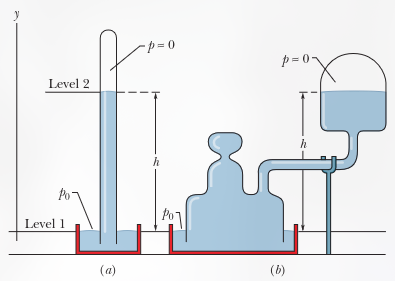
\includegraphics[width=0.45\linewidth]{images/25.png}
		\caption{Dua sumber bunyi $S_1$ dan $S_2$ (Gambar 17-38)}
	\end{figure}}{}

\diketahui\ ($S_1$ di titik asal sumbu $x$ dan $S_2$ berada $d$ dari $S_1$, tegak lurus sumbu $x$, menurut Gambar 17-38)
\begin{align*}
	\lambda & = \SI{2,00}{\metre}, &
	d       & = \SI{16,0}{\metre}.
\end{align*}
\ditanya\ (a) $\Delta\phi$ untuk $x\to\infty$; (b) jenis interferensi; (c) arah perubahan $\Delta\phi$; (d)--(f) $x$ untuk $\Delta\phi=0{,}50\lambda,\ 1{,}00\lambda,\ 1{,}50\lambda$.

\konsep\ Beda fase (dalam satuan panjang gelombang) sama dengan selisih lintasan dibagi $\lambda$: $\Delta\phi=\Delta L/\lambda$ dengan
\[
	\Delta L = \sqrt{x^2+d^2}-x
	\;\Rightarrow\;
	x=\frac{d^2-\Delta L^2}{2\,\Delta L}.
\]

\penyelesaian

\noindent\textbf{(a), (b) $P$ sangat jauh}

Untuk $x\to\infty$, $\sqrt{x^2+d^2}\to x$ sehingga $\Delta L\to0$:
\begin{align*}
	\Delta\phi & = 0,
\end{align*}
dan interferensi yang terjadi adalah \textbf{konstruktif penuh}.

\noindent\textbf{(c) $P$ mendekati $S_1$}

Makin kecil $x$, selisih $\sqrt{x^2+d^2}-x$ makin besar, sehingga beda fase \textbf{bertambah}.

\noindent\textbf{(d)--(f) Jarak $x$}
\begin{align*}
	\Delta\phi=0{,}50\lambda: & \quad \Delta L=\SI{1,00}{\metre},\quad x=\frac{(16{,}0)^2-(1{,}00)^2}{2(1{,}00)}\,\si{\metre}=\SI{127,5}{\metre}, \\
	\Delta\phi=1{,}00\lambda: & \quad \Delta L=\SI{2,00}{\metre},\quad x=\frac{(16{,}0)^2-(2{,}00)^2}{2(2{,}00)}\,\si{\metre}=\SI{63,0}{\metre},  \\
	\Delta\phi=1{,}50\lambda: & \quad \Delta L=\SI{3,00}{\metre},\quad x=\frac{(16{,}0)^2-(3{,}00)^2}{2(3{,}00)}\,\si{\metre}=\SI{41,2}{\metre}.
\end{align*}
\begin{jawaban}
	(a) $0$ \quad (b) konstruktif penuh \quad (c) bertambah \\
	(d) $\SI{127,5}{\metre}$ \quad (e) $\SI{63,0}{\metre}$ \quad (f) $\SI{41,2}{\metre}$.
\end{jawaban}

% ---------------------------------------------------------------------
\soal{28}
Dua bunyi memiliki taraf intensitas yang berbeda \SI{1,00}{\decibel}. Berapakah perbandingan intensitas yang lebih besar terhadap yang lebih kecil?

\diketahui
\begin{align*}
	\beta_2-\beta_1 & = \SI{1,00}{\decibel}.
\end{align*}
\ditanya\ $\dfrac{I_2}{I_1}$.

\konsep\ Taraf intensitas $\beta=(\SI{10}{\decibel})\log(I/I_0)$, sehingga selisih taraf intensitas dua bunyi tidak bergantung pada $I_0$:
$\beta_2-\beta_1=(\SI{10}{\decibel})\log(I_2/I_1)$.

\penyelesaian
\begin{align*}
	\beta_2-\beta_1 & = (\SI{10}{\decibel})\log\frac{I_2}{I_1}
	\;\Rightarrow\;
	\log\frac{I_2}{I_1}=\frac{\SI{1,00}{\decibel}}{\SI{10}{\decibel}}=0{,}100, \\
	\frac{I_2}{I_1} & = 10^{0{,}100} = 1{,}26.
\end{align*}
\begin{jawaban}
	\[
		\boxed{\frac{I_2}{I_1}\approx 1{,}26}
	\]
\end{jawaban}

% ---------------------------------------------------------------------
\soal{29}
Sebuah sumber memancarkan gelombang bunyi secara isotropik. Intensitas gelombang pada jarak \SI{2,50}{\metre} dari sumber adalah \SI{1,91e-4}{\watt\per\metre\squared}. Dengan anggapan energi gelombang kekal, tentukan daya sumber.

\diketahui
\begin{align*}
	r & = \SI{2,50}{\metre},                     &
	I & = \SI{1,91e-4}{\watt\per\metre\squared}.
\end{align*}
\ditanya\ Daya sumber $P_s$.

\konsep\ Untuk sumber titik isotropik, daya tersebar merata pada permukaan bola berjari-jari $r$: $I=\dfrac{P_s}{4\pi r^2}$.

\penyelesaian
\begin{align*}
	P_s & = I\,(4\pi r^2) = (\SI{1,91e-4}{\watt\per\metre\squared})\,4\pi(\SI{2,50}{\metre})^2 \\
	    & = \SI{1,50e-2}{\watt}.
\end{align*}
\begin{jawaban}
	\[
		\boxed{P_s\approx\SI{1,50e-2}{\watt}=\SI{15,0}{\milli\watt}}
	\]
\end{jawaban}

% ---------------------------------------------------------------------
\soal{40}
Pipa organa $A$, dengan kedua ujung terbuka, memiliki frekuensi fundamental \SI{300}{\hertz}. Harmonik ketiga pipa organa $B$, yang satu ujungnya terbuka, memiliki frekuensi yang sama dengan harmonik kedua pipa $A$. Berapa panjang (a) pipa $A$ dan (b) pipa $B$?

\diketahui\ (laju bunyi tidak disebut dalam soal, dipakai nilai baku $v=\SI{343}{\metre\per\second}$)
\begin{align*}
	f_{A,1} & = \SI{300}{\hertz},            &
	v       & = \SI{343}{\metre\per\second}.
\end{align*}
\ditanya\ (a) $L_A$; (b) $L_B$.

\konsep\ Pipa dengan kedua ujung terbuka: $f_n=\dfrac{nv}{2L}$ ($n=1,2,3,\dots$). Pipa dengan satu ujung tertutup: $f_m=\dfrac{mv}{4L}$ ($m=1,3,5,\dots$), sehingga harmonik ketiga ($m=3$) berfrekuensi $\dfrac{3v}{4L_B}$.

\penyelesaian

\noindent\textbf{(a) Panjang pipa $A$}
\begin{align*}
	f_{A,1} & = \frac{v}{2L_A}
	\;\Rightarrow\;
	L_A=\frac{v}{2f_{A,1}}=\frac{\SI{343}{\metre\per\second}}{2(\SI{300}{\hertz})}=\SI{0,572}{\metre}.
\end{align*}

\noindent\textbf{(b) Panjang pipa $B$}

Harmonik kedua pipa $A$ berfrekuensi $f_{A,2}=2f_{A,1}=\SI{600}{\hertz}$. Maka
\begin{align*}
	\frac{3v}{4L_B} & = \SI{600}{\hertz}
	\;\Rightarrow\;
	L_B=\frac{3v}{4(\SI{600}{\hertz})}=\frac{3(\SI{343}{\metre\per\second})}{2400\,\si{\per\second}}
	=\SI{0,429}{\metre}.
\end{align*}
\begin{jawaban}
	(a) $L_A \approx \SI{0,572}{\metre}$ \quad (b) $L_B \approx \SI{0,429}{\metre}$.
\end{jawaban}

% ---------------------------------------------------------------------
\soal{43}
Pada gambar soal, $S$ adalah pengeras suara kecil yang digerakkan osilator audio dengan frekuensi yang divariasikan dari \SI{1000}{\hertz} sampai \SI{2000}{\hertz}, dan $D$ adalah pipa silinder berujung terbuka dua-duanya dengan panjang \SI{45,7}{\centi\metre}. Laju bunyi dalam pipa berisi udara adalah \SI{344}{\metre\per\second}. (a) Pada berapa frekuensi bunyi dari pengeras suara menimbulkan resonansi dalam pipa? Berapa (b) frekuensi terendah dan (c) frekuensi terendah kedua yang menimbulkan resonansi?

\diketahui
\begin{align*}
	L & = \SI{0,457}{\metre},                      &
	v & = \SI{344}{\metre\per\second},             &
	f & \in [\SI{1000}{\hertz},\SI{2000}{\hertz}].
\end{align*}
\ditanya\ (a) Banyak frekuensi resonansi; (b) frekuensi terendah; (c) frekuensi terendah kedua.

\konsep\ Pipa dengan dua ujung terbuka beresonansi pada $f_n=\dfrac{nv}{2L}$, $n=1,2,3,\dots$

\penyelesaian

Frekuensi dasar pipa:
\begin{align*}
	f_1 & = \frac{v}{2L}=\frac{\SI{344}{\metre\per\second}}{2(\SI{0,457}{\metre})}=\SI{376}{\hertz}.
\end{align*}
Syarat $\SI{1000}{\hertz}\le nf_1\le\SI{2000}{\hertz}$ memberi $2{,}66\le n\le 5{,}31$, sehingga $n=3,4,5$:
\begin{align*}
	f_3 & = 3f_1 = \SI{1,13e3}{\hertz}, \\
	f_4 & = 4f_1 = \SI{1,51e3}{\hertz}, \\
	f_5 & = 5f_1 = \SI{1,88e3}{\hertz}.
\end{align*}
\begin{jawaban}
	(a) 3 frekuensi \quad (b) $\SI{1,13e3}{\hertz}$ \quad (c) $\SI{1,51e3}{\hertz}$.
\end{jawaban}

% ---------------------------------------------------------------------
\soal{51}
Senar $A$ sebuah biola agak terlalu kencang. Terdengar layangan \num{4,00} per sekon bila senar dibunyikan bersama garpu tala yang berosilasi tepat pada nada A konser (\SI{440}{\hertz}). Berapakah periode osilasi senar biola tersebut?

\diketahui
\begin{align*}
	f_{\text{garpu}}  & = \SI{440}{\hertz},  &
	f_{\text{layang}} & = \SI{4,00}{\hertz}.
\end{align*}
\ditanya\ Periode $T$ senar biola.

\konsep\ Frekuensi layangan $f_{\text{layang}}=|f_1-f_2|$. Senar yang terlalu kencang berfrekuensi lebih tinggi dari \SI{440}{\hertz}, sehingga $f_{\text{senar}}=f_{\text{garpu}}+f_{\text{layang}}$.

\penyelesaian
\begin{align*}
	f_{\text{senar}} & = \SI{440}{\hertz}+\SI{4,00}{\hertz}=\SI{444}{\hertz},                         \\
	T                & = \frac{1}{f_{\text{senar}}}=\frac{1}{\SI{444}{\hertz}}=\SI{2,25e-3}{\second}.
\end{align*}
\begin{jawaban}
	\[
		\boxed{T\approx\SI{2,25e-3}{\second}=\SI{2,25}{\milli\second}}
	\]
\end{jawaban}

% ---------------------------------------------------------------------
\soal{52}
Sebuah garpu tala berfrekuensi tidak diketahui menghasilkan \num{3,00} layangan per sekon dengan garpu tala standar berfrekuensi \SI{384}{\hertz}. Frekuensi layangan berkurang saat sepotong kecil lilin ditempelkan pada salah satu kaki garpu pertama. Berapakah frekuensi garpu tala tersebut?

\diketahui
\begin{align*}
	f_{\text{standar}} & = \SI{384}{\hertz},  &
	f_{\text{layang}}  & = \SI{3,00}{\hertz}.
\end{align*}
\ditanya\ Frekuensi garpu tala $f$.

\konsep\ $f_{\text{layang}}=|f-f_{\text{standar}}|$, sehingga $f=384\pm3$ Hz. Menempelkan lilin menambah massa kaki garpu, sehingga frekuensi garpu \textit{menurun}.

\penyelesaian

Setelah ditempeli lilin, $f$ turun dan frekuensi layangan ikut berkurang, berarti $f$ menjadi makin dekat ke \SI{384}{\hertz}. Hal ini hanya mungkin bila semula $f>384$ Hz:
\begin{align*}
	f & = \SI{384}{\hertz}+\SI{3,00}{\hertz}=\SI{387}{\hertz}.
\end{align*}
(Bila semula $f=\SI{381}{\hertz}$, penurunan $f$ akan menambah selisih dan layangan bertambah, bertentangan dengan soal.)
\begin{jawaban}
	\[
		\boxed{f=\SI{387}{\hertz}}
	\]
\end{jawaban}

% ---------------------------------------------------------------------
\soal{58}
Dua kereta bergerak saling mendekat dengan laju \SI{30,5}{\metre\per\second} relatif terhadap tanah. Salah satu kereta membunyikan peluit berfrekuensi \SI{500}{\hertz}. (a) Berapa frekuensi yang terdengar di kereta lain pada udara tenang? (b) Berapa frekuensi yang terdengar di kereta lain bila angin bertiup \SI{30,5}{\metre\per\second} menuju peluit dan menjauhi pendengar? (c) Berapa frekuensinya bila arah angin dibalik?

\diketahui\ (laju bunyi dipakai $v=\SI{343}{\metre\per\second}$)
\begin{align*}
	f                & = \SI{500}{\hertz},                                              &
	v_S=v_D          & = \SI{30,5}{\metre\per\second}\ (\text{relatif terhadap tanah}), &
	v_{\text{angin}} & = \SI{30,5}{\metre\per\second}.
\end{align*}
\ditanya\ (a) $f'$ udara tenang; (b) $f'$ angin menuju peluit; (c) $f'$ angin dibalik.

\konsep\ Efek Doppler dengan kecepatan sumber dan pendengar diukur \textit{relatif terhadap udara} (medium):
\[
	f'=f\,\frac{v+v_D}{v-v_S}\qquad
	(v_D,v_S\ \text{saling mendekat, relatif terhadap udara}).
\]

\penyelesaian

\noindent\textbf{(a) Udara tenang}
\begin{align*}
	f' & = f\,\frac{v+v_D}{v-v_S} = (\SI{500}{\hertz})\frac{343+30{,}5}{343-30{,}5}=\SI{598}{\hertz}.
\end{align*}

\noindent\textbf{(b) Angin menuju peluit, menjauhi pendengar}

Udara bergerak ke arah sumber. Relatif terhadap udara, sumber mendekati pendengar dengan laju $30{,}5+30{,}5=\SI{61,0}{\metre\per\second}$, sedangkan pendengar diam ($30{,}5-30{,}5=0$):
\begin{align*}
	f' & = f\,\frac{v+0}{v-61{,}0} = (\SI{500}{\hertz})\frac{343}{343-61{,}0}=\SI{608}{\hertz}.
\end{align*}

\noindent\textbf{(c) Arah angin dibalik}

Udara bergerak ke arah pendengar. Sumber diam relatif terhadap udara ($30{,}5-30{,}5=0$), sedangkan pendengar mendekati sumber dengan laju \SI{61,0}{\metre\per\second}:
\begin{align*}
	f' & = f\,\frac{v+61{,}0}{v-0} = (\SI{500}{\hertz})\frac{343+61{,}0}{343}=\SI{589}{\hertz}.
\end{align*}
\begin{jawaban}
	(a) $\SI{598}{\hertz}$ \quad (b) $\SI{608}{\hertz}$ \quad (c) $\SI{589}{\hertz}$.
\end{jawaban}

% ---------------------------------------------------------------------
\soal{70}
Sebuah pesawat terbang dengan laju $1{,}25$ kali laju bunyi. Dentuman sonik (\textit{sonic boom}) mencapai seseorang di tanah \SI{1,00}{\minute} setelah pesawat melintas tepat di atasnya. Berapa ketinggian pesawat? Anggap laju bunyi \SI{330}{\metre\per\second}.

\diketahui
\begin{align*}
	v_S & = 1{,}25\,v,                             &
	v   & = \SI{330}{\metre\per\second},           &
	t   & = \SI{1,00}{\minute}=\SI{60,0}{\second}.
\end{align*}
\ditanya\ Ketinggian $H$ pesawat.

\konsep\ Gelombang kejut membentuk kerucut Mach dengan setengah sudut $\theta$: $\sin\theta=\dfrac{v}{v_S}$. Dentuman tiba ketika permukaan kerucut melewati pengamat; saat itu pesawat telah bergerak sejauh $x=v_St$ dari posisi tepat di atas pengamat, dan $\tan\theta=\dfrac{H}{x}$.

\penyelesaian
\begin{align*}
	\sin\theta & = \frac{1}{1{,}25}=0{,}800
	\;\Rightarrow\;\theta=53{,}1^\circ,\qquad \tan\theta=\frac{0{,}800}{0{,}600}=1{,}33,                  \\
	x          & = v_St = 1{,}25(\SI{330}{\metre\per\second})(\SI{60,0}{\second}) = \SI{2,475e4}{\metre}, \\
	H          & = x\tan\theta = (\SI{2,475e4}{\metre})(1{,}33) = \SI{3,30e4}{\metre}.
\end{align*}
\begin{jawaban}
	\[
		\boxed{H\approx\SI{3,3e4}{\metre}=\SI{33}{\kilo\metre}}
	\]
\end{jawaban}

% ---------------------------------------------------------------------
\soal{79}
Pada Gambar 17-46, bunyi berpanjang gelombang \SI{0,850}{\metre} dipancarkan secara isotropik oleh sumber titik $S$. Sinar bunyi 1 menuju langsung ke detektor $D$ pada jarak $L=\SI{10,0}{\metre}$. Sinar bunyi 2 menuju $D$ melalui pantulan pada permukaan datar; pantulan terjadi pada garis bagi tegak lurus garis $SD$, pada jarak $d$ dari garis tersebut. Anggap pantulan menggeser fase gelombang sebesar $0{,}500\lambda$. Untuk nilai terkecil $d$ (selain nol) berapa bunyi langsung dan bunyi pantul tiba di $D$ (a) tepat berlawanan fase dan (b) tepat sefase?

\IfFileExists{images/79.png}{%
	\begin{figure}[H]
		\centering
		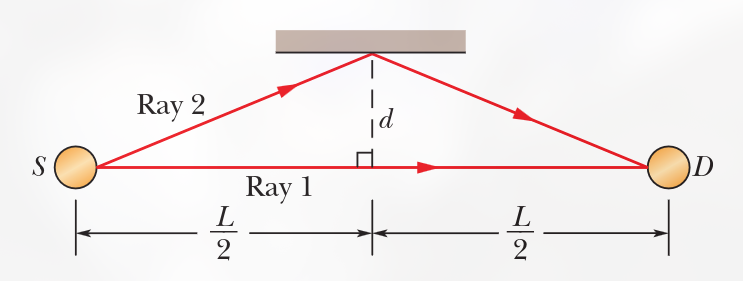
\includegraphics[width=0.45\linewidth]{images/79.png}
		\caption{Sinar langsung dan sinar pantul (Gambar 17-46)}
	\end{figure}}{}

\diketahui\ ($L$ dan pergeseran fase pantulan dibaca dari Gambar 17-46 dan teks soal)
\begin{align*}
	\lambda                    & = \SI{0,850}{\metre}, &
	L                          & = \SI{10,0}{\metre},  &
	\Delta\phi_{\text{pantul}} & = 0{,}500\lambda.
\end{align*}
\ditanya\ $d$ terkecil (bukan nol) untuk (a) berlawanan fase; (b) sefase.

\konsep\ Panjang lintasan sinar 2 adalah $2\sqrt{(L/2)^2+d^2}$, sehingga selisih lintasan
\[
	\Delta L = 2\sqrt{\left(\frac{L}{2}\right)^2+d^2}-L,
	\qquad
	d=\sqrt{\left(\frac{L+\Delta L}{2}\right)^2-\left(\frac{L}{2}\right)^2}.
\]
Beda fase total (dalam panjang gelombang) adalah $\Delta L/\lambda+0{,}5$.
Berlawanan fase: $\Delta L/\lambda+0{,}5=m+\tfrac12\Rightarrow\Delta L=m\lambda$.
Sefase: $\Delta L/\lambda+0{,}5=m\Rightarrow\Delta L=(m-\tfrac12)\lambda$.

\penyelesaian

\noindent\textbf{(a) Berlawanan fase}

$d=0$ ($\Delta L=0$) memang berlawanan fase, tetapi dikecualikan. Nilai terkecil berikutnya adalah $m=1$, yaitu $\Delta L=\lambda$:
\begin{align*}
	d & = \sqrt{\left(\frac{10{,}0+0{,}850}{2}\right)^2-\left(\frac{10{,}0}{2}\right)^2}\,\si{\metre}
	= \sqrt{29{,}43-25{,}0}\,\si{\metre}=\SI{2,10}{\metre}.
\end{align*}

\noindent\textbf{(b) Sefase}

Nilai terkecil: $m=1$, yaitu $\Delta L=\tfrac12\lambda=\SI{0,425}{\metre}$:
\begin{align*}
	d & = \sqrt{\left(\frac{10{,}0+0{,}425}{2}\right)^2-\left(\frac{10{,}0}{2}\right)^2}\,\si{\metre}
	= \sqrt{27{,}17-25{,}0}\,\si{\metre}=\SI{1,47}{\metre}.
\end{align*}
\begin{jawaban}
	(a) $d \approx \SI{2,10}{\metre}$ \quad (b) $d \approx \SI{1,47}{\metre}$.
\end{jawaban}

% =====================================================================
% BAB 18 -- SUHU, KALOR, DAN HUKUM PERTAMA TERMODINAMIKA
%           (potongan untuk ditempel ke main.tex)
% Memakai makro yang sudah ada di main.tex: \bab, \soal, rumusutama,
% \diketahui, \ditanya, \konsep, \penyelesaian, jawaban.
% =====================================================================
\bab{18}{Suhu, Kalor, dan Hukum Pertama Termodinamika}

\begin{rumusutama}
\begin{itemize}[nosep,leftmargin=*]
  \item \textbf{Skala suhu:}
        $T_C = T_K - \num{273,15}$, \quad $T_F = \tfrac{9}{5}T_C + 32$
  \item \textbf{Pemuaian termal:}
        $\Delta L = L\alpha\,\Delta T$, \quad $\Delta A = 2A\alpha\,\Delta T$, \quad
        $\Delta V = V\beta\,\Delta T$ \; ($\beta \approx 3\alpha$)
  \item \textbf{Kalor:}
        $Q = C\,\Delta T = cm\,\Delta T$; \quad perubahan fase $Q = Lm$;
        \quad kalor jenis molar $C=cM$
  \item \textbf{Asas Black (sistem terisolasi):}
        $\sum Q = 0$ (kalor yang dilepas = kalor yang diserap)
  \item \textbf{Usaha gas dan Hukum Pertama Termodinamika:}
        $W = \displaystyle\int_{V_i}^{V_f} p\,dV$, \quad
        $\Delta E_{\text{int}} = Q - W$
  \item \textbf{Perpindahan kalor:} konduksi
        $P_{\text{kond}} = \dfrac{Q}{t} = kA\,\dfrac{T_H - T_C}{L}$; radiasi
        $P_{\text{rad}} = \sigma\varepsilon A T^4$
\end{itemize}
\par\smallskip\noindent\footnotesize Rumus mengacu pada \cite{halliday}.
\end{rumusutama}

% ---------------------------------------------------------------------
\soal{13}
Tentukan perubahan volume sebuah bola aluminium berjari-jari awal \SI{10}{\centi\metre} ketika bola dipanaskan dari \SI{0,0}{\celsius} sampai \SI{100}{\celsius}.

\diketahui\ (koefisien muai linear aluminium dari Tabel 18-2)
\begin{align*}
r &= \SI{0,10}{\metre},&
\alpha_{\mathrm{Al}} &= \SI{23e-6}{\per\celsius},&
\Delta T &= \SI{100}{\celsius}.
\end{align*}
\ditanya\ $\Delta V$.

\konsep\ Pemuaian volume: $\Delta V=V\beta\,\Delta T$ dengan $\beta=3\alpha$.

\penyelesaian
\begin{align*}
V &= \frac43\pi r^3 = \frac43\pi(\SI{0,10}{\metre})^3 = \SI{4,19e-3}{\metre\cubed},\\
\beta &= 3\alpha = 3(\SI{23e-6}{\per\celsius}) = \SI{69e-6}{\per\celsius},\\
\Delta V &= V\beta\,\Delta T = (\SI{4,19e-3}{\metre\cubed})(\SI{69e-6}{\per\celsius})(\SI{100}{\celsius})
= \SI{2,9e-5}{\metre\cubed}.
\end{align*}
\begin{jawaban}
\[
\boxed{\Delta V \approx \SI{2,9e-5}{\metre\cubed}=\SI{29}{\centi\metre\cubed}}
\]
\end{jawaban}

% ---------------------------------------------------------------------
\soal{15}
Sebuah batang baja berdiameter \SI{3,000}{\centi\metre} pada \SI{25,00}{\celsius}. Sebuah cincin kuningan memiliki diameter dalam \SI{2,992}{\centi\metre} pada \SI{25,00}{\celsius}. Pada suhu bersama berapa cincin tepat dapat dimasukkan ke batang?

\diketahui\ (Tabel 18-2)
\begin{align*}
D_s &= \SI{3,000}{\centi\metre},&
D_b &= \SI{2,992}{\centi\metre},&
T_0 &= \SI{25,00}{\celsius},\\
\alpha_s &= \SI{11e-6}{\per\celsius},&
\alpha_b &= \SI{19e-6}{\per\celsius}.
\end{align*}
\ditanya\ Suhu bersama $T$ agar $D_s'=D_b'$.

\konsep\ Diameter memuai secara linear: $D'=D(1+\alpha\,\Delta T)$. Cincin kuningan memuai lebih cepat daripada batang baja, sehingga pada suhu tertentu diameter dalam cincin menjadi sama dengan diameter batang.

\penyelesaian
\begin{align*}
D_s(1+\alpha_s\Delta T) &= D_b(1+\alpha_b\Delta T),\\
D_s - D_b &= (D_b\alpha_b - D_s\alpha_s)\,\Delta T,\\
\Delta T &= \frac{\SI{3,000}{\centi\metre}-\SI{2,992}{\centi\metre}}
{(\SI{2,992}{\centi\metre})(\SI{19e-6}{\per\celsius})-(\SI{3,000}{\centi\metre})(\SI{11e-6}{\per\celsius})}\\
&= \frac{0{,}008}{\left(5{,}685-3{,}300\right)\times10^{-5}}\,\si{\celsius}=\SI{335}{\celsius},\\
T &= T_0+\Delta T = \SI{25,00}{\celsius}+\SI{335}{\celsius}=\SI{360}{\celsius}.
\end{align*}
\begin{jawaban}
\[
\boxed{T \approx \SI{360}{\celsius}}
\]
\end{jawaban}

% ---------------------------------------------------------------------
\soal{21}
Akibat kenaikan suhu sebesar \SI{32}{\celsius} (selisih suhu), sebuah batang dengan retakan di bagian tengahnya melengkung ke atas (Gambar 18-32). Jarak tetap $L_0$ antara kedua tumpuan adalah \SI{3,77}{\metre} dan koefisien muai linear batang adalah \SI{25e-6}{\per\celsius}. Tentukan kenaikan $x$ titik tengah batang.

\IfFileExists{images/21.png}{%
\begin{figure}[H]
  \centering
  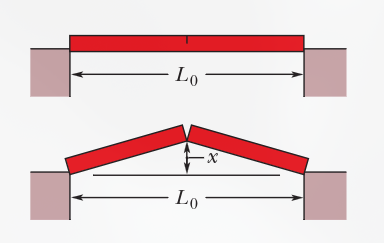
\includegraphics[width=0.45\linewidth]{images/21.png}
  \caption{Batang yang melengkung ke atas (Gambar 18-32)}
\end{figure}}{}

\diketahui\ ($L_0$ adalah jarak seluruh batang di antara kedua tumpuan, menurut Gambar 18-32)
\begin{align*}
L_0 &= \SI{3,77}{\metre},&
\alpha &= \SI{25e-6}{\per\celsius},&
\Delta T &= \SI{32}{\celsius}.
\end{align*}
\ditanya\ Kenaikan titik tengah $x$.

\konsep\ Setelah memuai, panjang batang menjadi $L=L_0(1+\alpha\Delta T)$, sedangkan jarak antartumpuan tetap $L_0$. Tiap setengah batang (panjang $L/2$) menjadi sisi miring segitiga siku-siku dengan alas $L_0/2$ dan tinggi $x$.

\penyelesaian
\begin{align*}
\alpha\Delta T &= (\SI{25e-6}{\per\celsius})(\SI{32}{\celsius}) = 8{,}0\times10^{-4},\\
\left(\frac{L}{2}\right)^2 &= \left(\frac{L_0}{2}\right)^2 + x^2
\;\Rightarrow\;
x = \frac{L_0}{2}\sqrt{(1+\alpha\Delta T)^2-1}\\
&\approx \frac{L_0}{2}\sqrt{2\alpha\Delta T}
= \frac{\SI{3,77}{\metre}}{2}\sqrt{2(8{,}0\times10^{-4})}\\
&= (\SI{1,885}{\metre})(0{,}0400) = \SI{7,5e-2}{\metre}.
\end{align*}
\begin{jawaban}
\[
\boxed{x \approx \SI{7,5}{\centi\metre}}
\]
\end{jawaban}

% ---------------------------------------------------------------------
\soal{30}
Sebuah sampel \SI{0,400}{\kilo\gram} ditempatkan pada alat pendingin yang mengambil energi sebagai kalor dengan laju tetap. Gambar 18-33 memperlihatkan suhu $T$ sampel terhadap waktu $t$; skala horizontal ditetapkan oleh $t_s=\SI{80,0}{\minute}$. Sampel membeku selama pengambilan energi. Kalor jenis sampel pada fase cair awal adalah \SI{3000}{\joule\per\kilo\gram\per\kelvin}. Tentukan (a) kalor lebur sampel dan (b) kalor jenisnya pada fase beku.

\IfFileExists{images/30.png}{%
\begin{figure}[H]
  \centering
  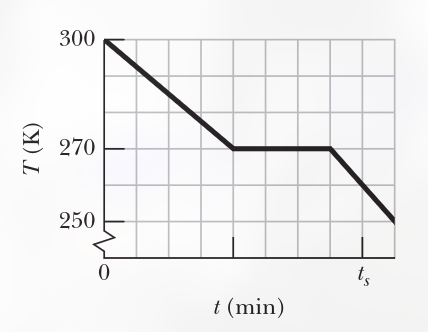
\includegraphics[width=0.5\linewidth]{images/30.png}
  \caption{Suhu sampel terhadap waktu (Gambar 18-33)}
\end{figure}}{}

\diketahui\ (dibaca dari Gambar 18-33; setiap kotak mendatar sebesar \SI{10}{\minute}: fase cair \SI{300}{\kelvin}$\to$\SI{270}{\kelvin} pada $t=0$ sampai \SI{40}{\minute}; pembekuan pada \SI{270}{\kelvin} dari \SI{40}{\minute} sampai \SI{70}{\minute}; fase padat \SI{270}{\kelvin}$\to$\SI{250}{\kelvin} dari \SI{70}{\minute} sampai \SI{80}{\minute})
\begin{align*}
m &= \SI{0,400}{\kilo\gram},&
c_{\text{cair}} &= \SI{3000}{\joule\per\kilo\gram\per\kelvin},\\
\Delta T_{\text{cair}} &= \SI{30}{\kelvin}\ (\Delta t = \SI{40}{\minute}),&
\Delta T_{\text{padat}} &= \SI{20}{\kelvin}\ (\Delta t = \SI{10}{\minute}),\\
\Delta t_{\text{beku}} &= \SI{30}{\minute}.
\end{align*}
\ditanya\ (a) $L_F$; (b) $c_{\text{padat}}$.

\konsep\ Laju pengambilan energi $P$ tetap, sehingga $Q=P\,\Delta t$ pada tiap selang. $P$ ditentukan dari fase cair: $P=c_{\text{cair}}m\,|\Delta T_{\text{cair}}|/\Delta t_{\text{cair}}$. Pada pembekuan $Q=L_Fm$ (suhu tetap), dan pada fase padat $Q=c_{\text{padat}}m|\Delta T_{\text{padat}}|$.

\penyelesaian

\noindent\textbf{Laju pengambilan energi (dari fase cair)}
\begin{align*}
P &= \frac{c_{\text{cair}}m|\Delta T_{\text{cair}}|}{\Delta t_{\text{cair}}}
= \frac{(\SI{3000}{\joule\per\kilo\gram\per\kelvin})(\SI{0,400}{\kilo\gram})(\SI{30}{\kelvin})}{2400\,\si{\second}}
= \SI{15,0}{\watt}.
\end{align*}

\noindent\textbf{(a) Kalor lebur}
\begin{align*}
Q_{\text{beku}} &= P\,\Delta t_{\text{beku}} = (\SI{15,0}{\watt})(1800\,\si{\second}) = \SI{2,70e4}{\joule},\\
L_F &= \frac{Q_{\text{beku}}}{m} = \frac{\SI{2,70e4}{\joule}}{\SI{0,400}{\kilo\gram}} = \SI{6,75e4}{\joule\per\kilo\gram}.
\end{align*}

\noindent\textbf{(b) Kalor jenis fase padat}
\begin{align*}
Q_{\text{padat}} &= P\,\Delta t_{\text{padat}} = (\SI{15,0}{\watt})(600\,\si{\second}) = \SI{9,0e3}{\joule},\\
c_{\text{padat}} &= \frac{Q_{\text{padat}}}{m|\Delta T_{\text{padat}}|}
= \frac{\SI{9,0e3}{\joule}}{(\SI{0,400}{\kilo\gram})(\SI{20}{\kelvin})}
= \SI{1,1e3}{\joule\per\kilo\gram\per\kelvin}.
\end{align*}
\begin{jawaban}
(a) $L_F \approx \SI{68}{\kilo\joule\per\kilo\gram}$ \quad
(b) $c_{\text{padat}} \approx \SI{1,1e3}{\joule\per\kilo\gram\per\kelvin}$.
\end{jawaban}

% ---------------------------------------------------------------------
\soal{35}
Sebuah termos terisolasi berisi \SI{130}{\centi\metre\cubed} kopi panas pada \SI{80,0}{\celsius}. Kamu memasukkan sebongkah es bermassa \SI{12,0}{\gram} pada titik leburnya untuk mendinginkan kopi. Berapa derajat kopi mendingin setelah es mencair dan kesetimbangan tercapai? Anggap kopi sebagai air murni dan abaikan pertukaran energi dengan lingkungan.

\diketahui\ (kalor jenis air dan kalor lebur es dari Tabel 18-3 dan 18-4; massa jenis air $\SI{1,00}{\gram\per\centi\metre\cubed}$)
\begin{align*}
m_k &= \SI{0,130}{\kilo\gram},&
T_k &= \SI{80,0}{\celsius},&
m_e &= \SI{0,0120}{\kilo\gram},\\
c &= \SI{4190}{\joule\per\kilo\gram\per\kelvin},&
L_F &= \SI{333}{\kilo\joule\per\kilo\gram}.
\end{align*}
\ditanya\ Penurunan suhu kopi $\Delta T_k = T_k - T_f$.

\konsep\ Sistem terisolasi: kalor yang dilepas kopi sama dengan kalor yang diserap es untuk melebur ($m_eL_F$) dan kemudian dipanaskan dari \SI{0}{\celsius} sampai $T_f$.

\penyelesaian
\begin{align*}
m_kc(T_k-T_f) &= m_eL_F + m_ec\,(T_f-0),\\
T_f &= \frac{m_kcT_k-m_eL_F}{(m_k+m_e)c}\\
&= \frac{(0{,}130)(4190)(80{,}0)-(0{,}0120)(3{,}33\times10^{5})}{(0{,}130+0{,}0120)(4190)}\,\si{\celsius}\\
&= \frac{43\,576-3996}{594{,}98}\,\si{\celsius}=\SI{66,5}{\celsius},\\
\Delta T_k &= \SI{80,0}{\celsius}-\SI{66,5}{\celsius}=\SI{13,5}{\celsius}.
\end{align*}
\begin{jawaban}
\[
\boxed{\Delta T_k \approx \SI{13,5}{\celsius}}\quad(T_f\approx\SI{66,5}{\celsius}).
\]
\end{jawaban}

% ---------------------------------------------------------------------
\soal{61}
Lapisan es setebal \SI{5,0}{\centi\metre} terbentuk di atas tangki air di luar ruangan (Gambar 18-47). Udara bersuhu \SI{-10}{\celsius}. Tentukan laju pembentukan es (dalam sentimeter per jam). Es memiliki konduktivitas termal $0{,}0040\ \mathrm{cal/(s\cdot cm\cdot C^\circ)}$ dan massa jenis \SI{0,92}{\gram\per\centi\metre\cubed}. Anggap tidak ada perpindahan energi melalui dinding atau dasar tangki.

\IfFileExists{images/61.png}{%
\begin{figure}[H]
  \centering
  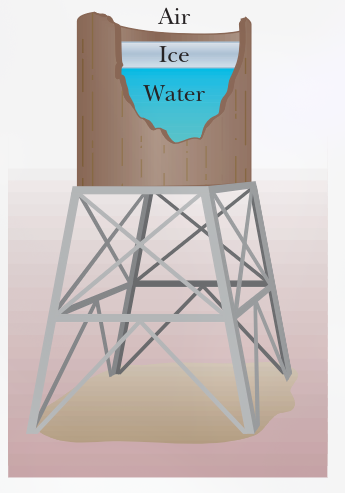
\includegraphics[width=0.35\linewidth]{images/61.png}
  \caption{Lapisan es di atas tangki air (Gambar 18-47)}
\end{figure}}{}

\diketahui\ (kalor lebur air $L_F=\SI{333}{\kilo\joule\per\kilo\gram}=79{,}5\ \mathrm{cal/g}$; permukaan bawah es berada pada \SI{0}{\celsius} karena berbatasan dengan air)
\begin{align*}
h &= \SI{5,0}{\centi\metre},&
T_{\text{udara}} &= \SI{-10}{\celsius},&
T_{\text{bawah}} &= \SI{0}{\celsius},\\
k &= 0{,}0040\ \mathrm{cal/(s\cdot cm\cdot C^\circ)},&
\rho &= \SI{0,92}{\gram\per\centi\metre\cubed},&
L_F &= 79{,}5\ \mathrm{cal/g}.
\end{align*}
\ditanya\ Laju pertumbuhan tebal es $dh/dt$.

\konsep\ Pada keadaan mantap, kalor yang dilepas air saat membeku di dasar lapisan es dikonduksikan ke atas melalui es: $P=kA\dfrac{\Delta T}{h}$. Massa es yang terbentuk per satuan waktu adalah $\dfrac{dm}{dt}=\rho A\dfrac{dh}{dt}$ dan kalor yang dilepas $P=L_F\dfrac{dm}{dt}$.

\penyelesaian
\begin{align*}
kA\frac{\Delta T}{h} &= L_F\rho A\frac{dh}{dt}
\;\Rightarrow\;
\frac{dh}{dt}=\frac{k\,\Delta T}{\rho L_F\,h}\\
&= \frac{(0{,}0040)(10)}{(0{,}92)(79{,}5)(5{,}0)}\,\si{\centi\metre\per\second}
= \SI{1,09e-4}{\centi\metre\per\second},\\
\frac{dh}{dt} &= (\SI{1,09e-4}{\centi\metre\per\second})(3600\,\si{\second\per\hour})
= \SI{0,39}{\centi\metre\per\hour}.
\end{align*}
\begin{jawaban}
\[
\boxed{\frac{dh}{dt}\approx\SI{0,39}{\centi\metre\per\hour}}
\]
\end{jawaban}

% ---------------------------------------------------------------------
\soal{82}
Sebuah batang tembaga, sebuah batang aluminium, dan sebuah batang kuningan, masing-masing berpanjang $L=\SI{6,00}{\metre}$ dan berdiameter $d=\SI{1,00}{\centi\metre}$, diletakkan berujung-ujung dengan batang aluminium berada di antara kedua batang lainnya. Ujung bebas batang tembaga dijaga pada titik didih air ($\SI{100}{\celsius}$) dan ujung bebas batang kuningan dijaga pada titik beku air ($\SI{0}{\celsius}$). Berapa suhu keadaan mantap (a) sambungan tembaga--aluminium dan (b) sambungan aluminium--kuningan?

\diketahui\ ($k$ dari Tabel 18-6; ukuran batang tidak memengaruhi hasil karena sama untuk ketiganya)
\begin{align*}
k_{\mathrm{Cu}} &= \SI{401}{\watt\per\metre\per\kelvin},&
k_{\mathrm{Al}} &= \SI{235}{\watt\per\metre\per\kelvin},&
k_{\mathrm{Br}} &= \SI{109}{\watt\per\metre\per\kelvin},\\
T_H &= \SI{100}{\celsius},&
T_C &= \SI{0}{\celsius}.
\end{align*}
\ditanya\ (a) $T_1$ (sambungan Cu--Al); (b) $T_2$ (sambungan Al--Br).

\konsep\ Pada keadaan mantap, laju konduksi kalor $P=kA\,\Delta T/L$ sama untuk ketiga batang. Karena $A$ dan $L$ sama, hambatan termal tiap batang sebanding dengan $1/k$ dan beda suhu terbagi sebanding dengan $1/k$.

\penyelesaian
\begin{align*}
P &= \frac{A}{L}\,\frac{T_H-T_C}{\dfrac{1}{k_{\mathrm{Cu}}}+\dfrac{1}{k_{\mathrm{Al}}}+\dfrac{1}{k_{\mathrm{Br}}}},\qquad
\sum\frac1k=\frac1{401}+\frac1{235}+\frac1{109}=0{,}01592\,\si{\metre\kelvin\per\watt},\\
\Delta T_{\mathrm{Cu}} &= (\SI{100}{\celsius})\,\frac{1/401}{0{,}01592}=\SI{15,7}{\celsius},\qquad
\Delta T_{\mathrm{Al}} = (\SI{100}{\celsius})\,\frac{1/235}{0{,}01592}=\SI{26,7}{\celsius},\\
T_1 &= T_H-\Delta T_{\mathrm{Cu}} = \SI{84,3}{\celsius},\\
T_2 &= T_1-\Delta T_{\mathrm{Al}} = \SI{57,6}{\celsius}.
\end{align*}
\begin{jawaban}
(a) $T_1 \approx \SI{84,3}{\celsius}$ \quad (b) $T_2 \approx \SI{57,6}{\celsius}$.
\end{jawaban}

% ---------------------------------------------------------------------
\soal{89}
Seorang atlet perlu menurunkan berat badan dan memutuskan melakukannya dengan "angkat besi". (a) Berapa kali beban \SI{80,0}{\kilo\gram} harus diangkat setinggi \SI{1,00}{\metre} untuk membakar $\num{1,00}$ lb lemak, dengan anggapan lemak sebanyak itu setara dengan $3500\ \text{Cal}$? (b) Jika beban diangkat sekali tiap \SI{2,00}{\second}, berapa lama pekerjaan itu berlangsung?

\diketahui\ ($1\ \text{Cal}=1\ \text{kkal}=\SI{4186}{\joule}$)
\begin{align*}
m &= \SI{80,0}{\kilo\gram},&
h &= \SI{1,00}{\metre},&
E &= 3500\ \text{Cal},&
\Delta t &= \SI{2,00}{\second}\text{ per angkatan}.
\end{align*}
\ditanya\ (a) Banyak angkatan $N$; (b) lama total $t$.

\konsep\ Kerja untuk satu angkatan adalah kenaikan energi potensial gravitasi $W_1=mgh$. Banyak angkatan $N=E/W_1$, dan lama total $t=N\,\Delta t$.

\penyelesaian

\noindent\textbf{(a) Banyak angkatan}
\begin{align*}
E &= (3500)(\SI{4186}{\joule}) = \SI{1,465e7}{\joule},\\
W_1 &= mgh = (\SI{80,0}{\kilo\gram})(\SI{9,8}{\metre\per\second\squared})(\SI{1,00}{\metre}) = \SI{784}{\joule},\\
N &= \frac{E}{W_1} = \frac{\SI{1,465e7}{\joule}}{\SI{784}{\joule}} = \num{1,87e4}.
\end{align*}

\noindent\textbf{(b) Lama pekerjaan}
\begin{align*}
t &= N\,\Delta t = (\num{1,87e4})(\SI{2,00}{\second}) = \SI{3,74e4}{\second} = \SI{10,4}{\hour}.
\end{align*}
\begin{jawaban}
(a) $N \approx \num{1,87e4}$ kali \quad (b) $t \approx \SI{10,4}{\hour}$.
\end{jawaban}

% ---------------------------------------------------------------------
\soal{96}
Gambar 18-59 memperlihatkan batang gabungan sepanjang $L=L_1+L_2$ yang terdiri atas dua bahan. Bahan pertama memiliki panjang $L_1$ dan koefisien muai linear $\alpha_1$; bahan kedua memiliki panjang $L_2$ dan koefisien $\alpha_2$. (a) Berapa koefisien muai linear $\alpha$ batang gabungan? Untuk batang gabungan tertentu, $L=\SI{52,4}{\centi\metre}$, bahan 1 adalah baja, dan bahan 2 adalah kuningan. Jika $\alpha=\SI{1,3e-5}{\per\celsius}$, berapa panjang (b) $L_1$ dan (c) $L_2$?

\IfFileExists{images/96.png}{%
\begin{figure}[H]
  \centering
  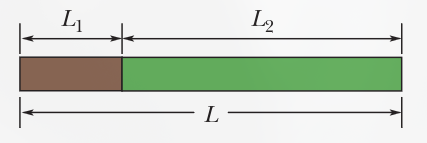
\includegraphics[width=0.4\linewidth]{images/96.png}
  \caption{Batang gabungan dua bahan (Gambar 18-59)}
\end{figure}}{}

\diketahui\ ($\alpha$ dari Tabel 18-2)
\begin{align*}
L &= \SI{52,4}{\centi\metre},&
\alpha &= \SI{13e-6}{\per\celsius},\\
\alpha_{\text{baja}} &= \SI{11e-6}{\per\celsius},&
\alpha_{\text{kuningan}} &= \SI{19e-6}{\per\celsius}.
\end{align*}
\ditanya\ (a) $\alpha$ dalam $\alpha_1,\alpha_2,L_1,L_2$; (b) $L_1$; (c) $L_2$.

\konsep\ Pertambahan panjang total sama dengan jumlah pertambahan panjang tiap bahan: $\Delta L=\Delta L_1+\Delta L_2$, dengan $\Delta L=\alpha L\,\Delta T$.

\penyelesaian

\noindent\textbf{(a) Koefisien muai gabungan}
\begin{align*}
\alpha L\,\Delta T &= \alpha_1L_1\,\Delta T+\alpha_2L_2\,\Delta T
\;\Rightarrow\;
\alpha=\frac{\alpha_1L_1+\alpha_2L_2}{L}.
\end{align*}

\noindent\textbf{(b), (c) Panjang masing-masing bahan}

Dengan $L_2=L-L_1$:
\begin{align*}
\alpha L &= \alpha_1L_1+\alpha_2(L-L_1)
\;\Rightarrow\;
L_1=L\,\frac{\alpha_2-\alpha}{\alpha_2-\alpha_1}\\
&= (\SI{52,4}{\centi\metre})\frac{19-13}{19-11} = \SI{39,3}{\centi\metre},\\
L_2 &= L-L_1 = \SI{52,4}{\centi\metre}-\SI{39,3}{\centi\metre} = \SI{13,1}{\centi\metre}.
\end{align*}
\begin{jawaban}
(a) $\alpha=\dfrac{\alpha_1L_1+\alpha_2L_2}{L}$ \quad
(b) $L_1\approx\SI{39,3}{\centi\metre}$ \quad (c) $L_2\approx\SI{13,1}{\centi\metre}$.
\end{jawaban}

% ---------------------------------------------------------------------
\soal{103}
Luas pelat persegi panjang adalah $A=ab=\SI{1,4}{\metre\squared}$ dan koefisien muai liniernya $\alpha=\SI{32e-6}{\per\celsius}$. Setelah kenaikan suhu $\Delta T=\SI{89}{\celsius}$, sisi $a$ bertambah panjang sebesar $\Delta a$ dan sisi $b$ sebesar $\Delta b$ (Gambar 18-61). Dengan mengabaikan besaran kecil $(\Delta a\,\Delta b)/(ab)$, tentukan $\Delta A$.

\diketahui
\begin{align*}
A &= ab = \SI{1,4}{\metre\squared},&
\alpha &= \SI{32e-6}{\per\celsius},&
\Delta T &= \SI{89}{\celsius}.
\end{align*}
\ditanya\ Pertambahan luas $\Delta A$.

\konsep\ $A'=(a+\Delta a)(b+\Delta b)$ dengan $\Delta a=a\alpha\Delta T$ dan $\Delta b=b\alpha\Delta T$.

\penyelesaian
\begin{align*}
\Delta A &= (a+\Delta a)(b+\Delta b)-ab = a\,\Delta b+b\,\Delta a+\Delta a\,\Delta b\\
&\approx a\,\Delta b+b\,\Delta a \qquad(\Delta a\,\Delta b\ \text{diabaikan})\\
&= ab\,\alpha\Delta T+ab\,\alpha\Delta T = 2A\alpha\,\Delta T\\
&= 2(\SI{1,4}{\metre\squared})(\SI{32e-6}{\per\celsius})(\SI{89}{\celsius})
= \SI{8,0e-3}{\metre\squared}.
\end{align*}
\begin{jawaban}
\[
\boxed{\Delta A \approx \SI{8,0e-3}{\metre\squared}}
\]
\end{jawaban}

% =====================================================================
% BAB 19 -- TEORI KINETIK GAS   (potongan untuk ditempel ke main.tex)
% Memakai makro yang sudah ada di main.tex: \bab, \soal, rumusutama,
% \diketahui, \ditanya, \konsep, \penyelesaian, jawaban.
% Tempel setelah Bab 18 dan sebelum Bab 20.
% =====================================================================
\bab{19}{Teori Kinetik Gas}

\begin{rumusutama}
\begin{itemize}[nosep,leftmargin=*]
  \item \textbf{Hukum gas ideal:}
        $pV = nRT = NkT$, \quad $R = \SI{8,31}{\joule\per\mole\per\kelvin}$,
        \; $k = \SI{1,38e-23}{\joule\per\kelvin}$
  \item \textbf{Kelajuan dan energi kinetik molekul:}
        $v_{\text{rms}} = \sqrt{\dfrac{3RT}{M}}$, \quad
        $K_{\text{rata}} = \tfrac{3}{2}kT$
  \item \textbf{Lintasan bebas rata-rata:}
        $\lambda = \dfrac{1}{\sqrt{2}\,\pi d^2\,N/V}$
  \item \textbf{Kalor jenis molar gas ideal:}
        $E_{\text{int}} = nC_V T$, \quad $\Delta E_{\text{int}} = nC_V\,\Delta T$, \quad
        $C_p = C_V + R$ \\
        ($C_V = \tfrac{3}{2}R$ monoatomik; $C_V = \tfrac{5}{2}R$ diatomik)
  \item \textbf{Proses adiabatik:}
        $pV^{\gamma} = \text{konstan}$, \quad
        $TV^{\gamma - 1} = \text{konstan}$, \quad $\gamma = \dfrac{C_p}{C_V}$
\end{itemize}
\par\smallskip\noindent\footnotesize Rumus mengacu pada \cite{halliday}.
\end{rumusutama}

% ---------------------------------------------------------------------
\soal{18}
Suhu dan tekanan di atmosfer Matahari adalah \SI{2,00e6}{\kelvin} dan \SI{0,0300}{\pascal}. Hitung laju rms elektron bebas (massa \SI{9,11e-31}{\kilo\gram}) di sana, dengan menganggapnya gas ideal.

\diketahui
\begin{align*}
T &= \SI{2,00e6}{\kelvin},&
p &= \SI{0,0300}{\pascal},&
m &= \SI{9,11e-31}{\kilo\gram}.
\end{align*}
\ditanya\ $v_{\text{rms}}$ elektron.

\konsep\ Untuk gas ideal, $\tfrac12 m v_{\text{rms}}^2=\tfrac32kT$, sehingga $v_{\text{rms}}=\sqrt{3kT/m}$. Tekanan tidak diperlukan, karena laju rms hanya bergantung pada suhu dan massa partikel.

\penyelesaian
\begin{align*}
v_{\text{rms}} &= \sqrt{\frac{3kT}{m}}
= \sqrt{\frac{3(\SI{1,38e-23}{\joule\per\kelvin})(\SI{2,00e6}{\kelvin})}{\SI{9,11e-31}{\kilo\gram}}}
= \SI{9,53e6}{\metre\per\second}.
\end{align*}
\begin{jawaban}
\[
\boxed{v_{\text{rms}}\approx\SI{9,53e6}{\metre\per\second}}
\]
\end{jawaban}

% ---------------------------------------------------------------------
\soal{28}
Pada frekuensi berapa panjang gelombang bunyi di udara sama dengan lintasan bebas rata-rata molekul oksigen pada tekanan \SI{1,0}{\atm} dan suhu \SI{0,00}{\celsius}? Diameter molekul adalah \SI{3,0e-8}{\centi\metre}.

\diketahui\ (laju bunyi tidak disebut dalam soal, dipakai nilai baku $v=\SI{343}{\metre\per\second}$)
\begin{align*}
p &= \SI{1,01e5}{\pascal},&
T &= \SI{273}{\kelvin},&
d &= \SI{3,0e-10}{\metre},&
v &= \SI{343}{\metre\per\second}.
\end{align*}
\ditanya\ Frekuensi $f$ saat $\lambda_{\text{bunyi}}=\lambda_{\text{lbr}}$.

\konsep\ Lintasan bebas rata-rata $\lambda_{\text{lbr}}=\dfrac{1}{\sqrt2\,\pi d^2\,N/V}$, dengan rapat molekul dari hukum gas ideal $\dfrac{N}{V}=\dfrac{p}{kT}$. Frekuensi bunyi $f=v/\lambda$.

\penyelesaian
\begin{align*}
\frac{N}{V} &= \frac{p}{kT} = \frac{\SI{1,01e5}{\pascal}}{(\SI{1,38e-23}{\joule\per\kelvin})(\SI{273}{\kelvin})}
= \SI{2,68e25}{\per\metre\cubed},\\
\lambda_{\text{lbr}} &= \frac{1}{\sqrt2\,\pi\,(\SI{3,0e-10}{\metre})^2(\SI{2,68e25}{\per\metre\cubed})}
= \SI{9,3e-8}{\metre},\\
f &= \frac{v}{\lambda_{\text{lbr}}} = \frac{\SI{343}{\metre\per\second}}{\SI{9,3e-8}{\metre}}
= \SI{3,7e9}{\hertz}.
\end{align*}
\begin{jawaban}
\[
\boxed{f \approx \SI{3,7e9}{\hertz}}
\]
\end{jawaban}

% ---------------------------------------------------------------------
\soal{30}
Lintasan bebas rata-rata molekul nitrogen pada \SI{0,0}{\celsius} dan \SI{1,0}{\atm} adalah \SI{0,80e-5}{\centi\metre}. Pada suhu dan tekanan ini terdapat $2{,}7\times10^{19}$ molekul$/\mathrm{cm^3}$. Berapa diameter molekul?

\diketahui
\begin{align*}
\lambda &= \SI{0,80e-5}{\centi\metre}=\SI{8,0e-8}{\metre},&
\frac{N}{V} &= \SI{2,7e19}{\per\centi\metre\cubed}=\SI{2,7e25}{\per\metre\cubed}.
\end{align*}
\ditanya\ Diameter molekul $d$.

\konsep\ Lintasan bebas rata-rata $\lambda=\dfrac{1}{\sqrt2\,\pi d^2\,N/V}$, sehingga $d=\sqrt{\dfrac{1}{\sqrt2\,\pi\,\lambda\,(N/V)}}$.

\penyelesaian
\begin{align*}
d &= \sqrt{\frac{1}{\sqrt2\,\pi\,(\SI{8,0e-8}{\metre})(\SI{2,7e25}{\per\metre\cubed})}}
= \sqrt{\frac{1}{9{,}6\times10^{18}}}\,\si{\metre}\\
&= \SI{3,2e-10}{\metre}.
\end{align*}
\begin{jawaban}
\[
\boxed{d\approx\SI{3,2e-10}{\metre}=\SI{3,2e-8}{\centi\metre}}
\]
\end{jawaban}

% ---------------------------------------------------------------------
\soal{33}
Laju \num{10} molekul adalah \num{2,0}, \num{3,0}, \num{4,0}, \dots, \SI{11}{\kilo\metre\per\second}. Berapa (a) laju rata-rata dan (b) laju rms molekul-molekul tersebut?

\diketahui
\begin{align*}
v_i &= 2{,}0;\ 3{,}0;\ 4{,}0;\ \dots;\ 11\ \si{\kilo\metre\per\second},&
N &= 10.
\end{align*}
\ditanya\ (a) $v_{\text{rata}}$; (b) $v_{\text{rms}}$.

\konsep\ $v_{\text{rata}}=\dfrac{1}{N}\sum v_i$ dan $v_{\text{rms}}=\sqrt{\dfrac{1}{N}\sum v_i^2}$.

\penyelesaian

\noindent\textbf{(a) Laju rata-rata}
\begin{align*}
\sum v_i &= 2+3+\cdots+11 = 65\ \si{\kilo\metre\per\second},\\
v_{\text{rata}} &= \frac{65}{10}\,\si{\kilo\metre\per\second} = \SI{6,5}{\kilo\metre\per\second}.
\end{align*}

\noindent\textbf{(b) Laju rms}
\begin{align*}
\sum v_i^2 &= 2^2+3^2+\cdots+11^2 = 505\ \si{\kilo\metre\squared\per\second\squared},\\
v_{\text{rms}} &= \sqrt{\frac{505}{10}}\,\si{\kilo\metre\per\second} = \SI{7,1}{\kilo\metre\per\second}.
\end{align*}
\begin{jawaban}
(a) $v_{\text{rata}} = \SI{6,5}{\kilo\metre\per\second}$ \quad (b) $v_{\text{rms}} \approx \SI{7,1}{\kilo\metre\per\second}$.
\end{jawaban}

% ---------------------------------------------------------------------
\soal{44}
Satu mol gas ideal diatomik bergerak dari $a$ ke $c$ sepanjang lintasan diagonal pada Gambar 19-25. Skala sumbu vertikal ditetapkan oleh $p_{ab}=\SI{5,0}{\kilo\pascal}$ dan $p_c=\SI{2,0}{\kilo\pascal}$, dan skala sumbu horizontal oleh $V_{bc}=\SI{4,0}{\metre\cubed}$ dan $V_a=\SI{2,0}{\metre\cubed}$. Selama transisi, (a) berapa perubahan energi dalam gas, dan (b) berapa banyak energi yang ditambahkan ke gas sebagai kalor? (c) Berapa kalor yang diperlukan bila gas bergerak dari $a$ ke $c$ melalui lintasan tidak langsung $abc$?

\IfFileExists{images/44.png}{%
\begin{figure}[H]
  \centering
  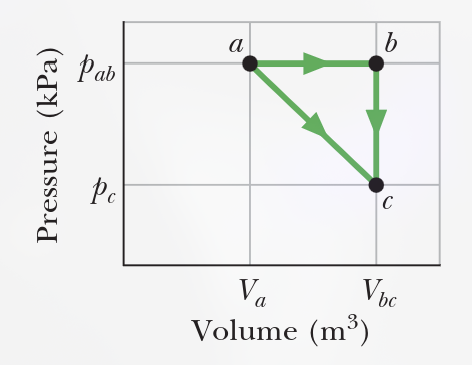
\includegraphics[width=0.4\linewidth]{images/44.png}
  \caption{Diagram $p$-$V$ gas diatomik (Gambar 19-25)}
\end{figure}}{}

\diketahui\ (dari Gambar 19-25: $a=(V_a,p_{ab})$, $b=(V_{bc},p_{ab})$, $c=(V_{bc},p_c)$)
\begin{align*}
p_{ab} &= \SI{5,0}{\kilo\pascal},&
p_c &= \SI{2,0}{\kilo\pascal},&
V_a &= \SI{2,0}{\metre\cubed},&
V_{bc} &= \SI{4,0}{\metre\cubed},&
n &= \SI{1}{\mole}.
\end{align*}
\ditanya\ (a) $\Delta E_{\text{int}}$ ($a\to c$); (b) $Q$ ($a\to c$ diagonal); (c) $Q$ lewat $abc$.

\konsep\ Untuk gas ideal diatomik ($C_V=\tfrac52R$), $\Delta E_{\text{int}}=nC_V\Delta T=\tfrac52(p_fV_f-p_iV_i)$, hanya bergantung pada keadaan awal dan akhir. Usaha oleh gas sama dengan luas di bawah kurva pada diagram $p$-$V$, dan $Q=\Delta E_{\text{int}}+W$.

\penyelesaian

\noindent\textbf{(a) Perubahan energi dalam}
\begin{align*}
\Delta E_{\text{int}} &= \tfrac52\left(p_cV_{bc}-p_{ab}V_a\right)
= \tfrac52\left[(\SI{2,0e3}{\pascal})(\SI{4,0}{\metre\cubed})-(\SI{5,0e3}{\pascal})(\SI{2,0}{\metre\cubed})\right]\\
&= \tfrac52(8{,}0-10{,}0)\times10^3\,\si{\joule} = -\SI{5,0e3}{\joule}.
\end{align*}

\noindent\textbf{(b) Kalor sepanjang lintasan diagonal}

Usaha adalah luas trapesium di bawah garis $a\to c$:
\begin{align*}
W_{ac} &= \tfrac12(p_{ab}+p_c)(V_{bc}-V_a) = \tfrac12(\SI{7,0e3}{\pascal})(\SI{2,0}{\metre\cubed}) = \SI{7,0e3}{\joule},\\
Q_{ac} &= \Delta E_{\text{int}}+W_{ac} = -\SI{5,0e3}{\joule}+\SI{7,0e3}{\joule} = \SI{2,0e3}{\joule}.
\end{align*}

\noindent\textbf{(c) Kalor sepanjang lintasan $abc$}

Usaha hanya terjadi pada $a\to b$ (tekanan tetap); $b\to c$ berlangsung pada volume tetap ($W=0$):
\begin{align*}
W_{abc} &= p_{ab}(V_{bc}-V_a) = (\SI{5,0e3}{\pascal})(\SI{2,0}{\metre\cubed}) = \SI{1,0e4}{\joule},\\
Q_{abc} &= \Delta E_{\text{int}}+W_{abc} = -\SI{5,0e3}{\joule}+\SI{1,0e4}{\joule} = \SI{5,0e3}{\joule}.
\end{align*}
\begin{jawaban}
(a) $\Delta E_{\text{int}}=-\SI{5,0}{\kilo\joule}$ \quad
(b) $Q=\SI{2,0}{\kilo\joule}$ \quad
(c) $Q=\SI{5,0}{\kilo\joule}$.
\end{jawaban}

% ---------------------------------------------------------------------
\soal{55}
Sebuah gas menempati volume \SI{4,3}{\litre} pada tekanan \SI{1,2}{\atm} dan suhu \SI{310}{\kelvin}. Gas dimampatkan secara adiabatik sampai volumenya \SI{0,76}{\litre}. Tentukan (a) tekanan akhir dan (b) suhu akhir, dengan menganggap gas sebagai gas ideal dengan $\gamma=\num{1,4}$.

\diketahui\ ($\gamma$ dari teks soal edisi 10)
\begin{align*}
V_i &= \SI{4,3}{\litre},&
p_i &= \SI{1,2}{\atm},&
T_i &= \SI{310}{\kelvin},&
V_f &= \SI{0,76}{\litre},&
\gamma &= \num{1,4}.
\end{align*}
\ditanya\ (a) $p_f$; (b) $T_f$.

\konsep\ Pada proses adiabatik gas ideal berlaku $pV^{\gamma}=\text{konstan}$ dan $TV^{\gamma-1}=\text{konstan}$.

\penyelesaian

\noindent\textbf{(a) Tekanan akhir}
\begin{align*}
p_f &= p_i\left(\frac{V_i}{V_f}\right)^{\gamma}
= (\SI{1,2}{\atm})\left(\frac{4{,}3}{0{,}76}\right)^{1{,}4}
= \SI{13,6}{\atm}\approx\SI{14}{\atm}.
\end{align*}

\noindent\textbf{(b) Suhu akhir}
\begin{align*}
T_f &= T_i\left(\frac{V_i}{V_f}\right)^{\gamma-1}
= (\SI{310}{\kelvin})\left(\frac{4{,}3}{0{,}76}\right)^{0{,}4}
= \SI{620}{\kelvin}.
\end{align*}
\begin{jawaban}
(a) $p_f \approx \SI{14}{\atm}$ ($\SI{13,6}{\atm}$) \quad (b) $T_f \approx \SI{6,2e2}{\kelvin}$.
\end{jawaban}

% ---------------------------------------------------------------------
\soal{63}
Gambar 19-27 memperlihatkan siklus yang dijalani \SI{1,00}{\mole} gas ideal monoatomik. Suhunya $T_1=\SI{300}{\kelvin}$, $T_2=\SI{600}{\kelvin}$, dan $T_3=\SI{455}{\kelvin}$. Untuk $1\to2$, berapa (a) kalor $Q$, (b) perubahan energi dalam $\Delta E_{\text{int}}$, dan (c) usaha $W$ oleh gas? Untuk $2\to3$, berapa (d) $Q$, (e) $\Delta E_{\text{int}}$, dan (f) $W$? Untuk $3\to1$, berapa (g) $Q$, (h) $\Delta E_{\text{int}}$, dan (i) $W$? Untuk satu siklus penuh, berapa (j) $Q$, (k) $\Delta E_{\text{int}}$, dan (l) $W$? Tekanan awal di titik 1 adalah \SI{1,00}{\atm} ($=\SI{1,013e5}{\pascal}$). Berapa (m) volume dan (n) tekanan di titik 2, serta (o) volume dan (p) tekanan di titik 3?

\IfFileExists{images/63.png}{%
\begin{figure}[H]
  \centering
  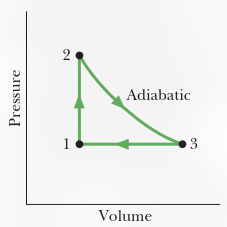
\includegraphics[width=0.4\linewidth]{images/63.png}
  \caption{Siklus gas ideal monoatomik (Gambar 19-27)}
\end{figure}}{}

\diketahui\ (dari Gambar 19-27: $1\to2$ volume tetap, $2\to3$ adiabatik, $3\to1$ tekanan tetap)
\begin{align*}
n &= \SI{1,00}{\mole},&
T_1 &= \SI{300}{\kelvin},&
T_2 &= \SI{600}{\kelvin},\\
T_3 &= \SI{455}{\kelvin},&
p_1 &= \SI{1,013e5}{\pascal}.
\end{align*}
\ditanya\ $Q$, $\Delta E_{\text{int}}$, $W$ tiap proses dan satu siklus; $V_2$, $p_2$, $V_3$, $p_3$.

\konsep\ Gas monoatomik: $C_V=\tfrac32R$ dan $C_p=\tfrac52R$. $\Delta E_{\text{int}}=nC_V\Delta T$ untuk semua proses, $Q=nC_V\Delta T$ (volume tetap), $Q=nC_p\Delta T$ (tekanan tetap), $Q=0$ (adiabatik), dan $W=Q-\Delta E_{\text{int}}$.

\penyelesaian

\noindent\textbf{Proses $1\to2$ (volume tetap)}
\begin{align*}
W_{12} &= 0,\\
\Delta E_{\text{int},12} &= nC_V(T_2-T_1) = (1{,}00)(\tfrac32)(8{,}314)(300)\,\si{\joule} = \SI{3,74e3}{\joule},\\
Q_{12} &= \Delta E_{\text{int},12} = \SI{3,74e3}{\joule}.
\end{align*}

\noindent\textbf{Proses $2\to3$ (adiabatik)}
\begin{align*}
Q_{23} &= 0,\\
\Delta E_{\text{int},23} &= nC_V(T_3-T_2) = (\tfrac32)(8{,}314)(455-600)\,\si{\joule} = -\SI{1,81e3}{\joule},\\
W_{23} &= -\Delta E_{\text{int},23} = \SI{1,81e3}{\joule}.
\end{align*}

\noindent\textbf{Proses $3\to1$ (tekanan tetap)}
\begin{align*}
\Delta E_{\text{int},31} &= nC_V(T_1-T_3) = (\tfrac32)(8{,}314)(300-455)\,\si{\joule} = -\SI{1,93e3}{\joule},\\
Q_{31} &= nC_p(T_1-T_3) = (\tfrac52)(8{,}314)(300-455)\,\si{\joule} = -\SI{3,22e3}{\joule},\\
W_{31} &= Q_{31}-\Delta E_{\text{int},31} = -\SI{1,29e3}{\joule}\quad(=nR(T_1-T_3)).
\end{align*}

\noindent\textbf{Satu siklus penuh}
\begin{align*}
Q &= 3{,}74-0-3{,}22 = \SI{5,2e2}{\joule},\\
\Delta E_{\text{int}} &= 3{,}74-1{,}81-1{,}93 = 0,\\
W &= 0+1{,}81-1{,}29 = \SI{5,2e2}{\joule}.
\end{align*}

\noindent\textbf{Volume dan tekanan}
\begin{align*}
V_1 &= \frac{nRT_1}{p_1} = \frac{(1{,}00)(8{,}314)(300)}{\SI{1,013e5}{\pascal}}\,\si{\metre\cubed} = \SI{2,46e-2}{\metre\cubed},\\
V_2 &= V_1 = \SI{2,46e-2}{\metre\cubed},\\
p_2 &= p_1\frac{T_2}{T_1} = \SI{2,03e5}{\pascal}\;(=\SI{2,00}{\atm}),\\
p_3 &= p_1 = \SI{1,013e5}{\pascal}\;(=\SI{1,00}{\atm}),\\
V_3 &= \frac{nRT_3}{p_3} = \frac{(1{,}00)(8{,}314)(455)}{\SI{1,013e5}{\pascal}}\,\si{\metre\cubed} = \SI{3,73e-2}{\metre\cubed}.
\end{align*}
\begin{jawaban}
\small\setlength{\tabcolsep}{4pt}
\begin{tabular}{@{}lccc@{}}
 & $Q$ (J) & $\Delta E_{\text{int}}$ (J) & $W$ (J) \\
$1\to2$ (a--c) & \num{3,74e3} & \num{3,74e3} & $0$ \\
$2\to3$ (d--f) & $0$ & $-\num{1,81e3}$ & \num{1,81e3} \\
$3\to1$ (g--i) & $-\num{3,22e3}$ & $-\num{1,93e3}$ & $-\num{1,29e3}$ \\
Siklus (j--l) & \num{5,2e2} & $0$ & \num{5,2e2} \\
\end{tabular}

(m) $V_2=\SI{2,46e-2}{\metre\cubed}$ \quad (n) $p_2=\SI{2,03e5}{\pascal}$ (\SI{2,00}{\atm}) \quad
(o) $V_3=\SI{3,73e-2}{\metre\cubed}$ \quad (p) $p_3=\SI{1,013e5}{\pascal}$ (\SI{1,00}{\atm}).
\end{jawaban}

% ---------------------------------------------------------------------
\soal{64}
Hitung usaha yang dilakukan oleh agen luar selama pemampatan isotermal \SI{1,00}{\mole} oksigen dari volume \SI{22,4}{\litre} pada \SI{0}{\celsius} dan \SI{1,00}{\atm} menjadi volume \SI{16,8}{\litre}.

\diketahui
\begin{align*}
n &= \SI{1,00}{\mole},&
T &= \SI{273}{\kelvin},&
V_i &= \SI{22,4}{\litre},&
V_f &= \SI{16,8}{\litre}.
\end{align*}
\ditanya\ Usaha oleh agen luar $W_{\text{luar}}$.

\konsep\ Usaha oleh gas pada proses isotermal: $W_{\text{gas}}=nRT\ln\dfrac{V_f}{V_i}$. Usaha oleh agen luar sama besar dengan $-W_{\text{gas}}$.

\penyelesaian
\begin{align*}
W_{\text{gas}} &= nRT\ln\frac{V_f}{V_i}
= (1{,}00)(\SI{8,31}{\joule\per\mole\per\kelvin})(\SI{273}{\kelvin})\ln\frac{16{,}8}{22{,}4}\\
&= (\SI{2,27e3}{\joule})(-0{,}288) = -\SI{653}{\joule},\\
W_{\text{luar}} &= -W_{\text{gas}} = +\SI{653}{\joule}.
\end{align*}
\begin{jawaban}
\[
\boxed{W_{\text{luar}}\approx\SI{653}{\joule}}
\]
(gas melakukan usaha $-\SI{653}{\joule}$ karena dimampatkan).
\end{jawaban}

% ---------------------------------------------------------------------
\soal{75}
Suhu \SI{3,00}{\mole} suatu gas dengan $C_V=6{,}00\ \mathrm{cal/mol\cdot K}$ akan dinaikkan sebesar \SI{50,0}{\kelvin}. Jika prosesnya pada volume tetap, berapa (a) energi yang dipindahkan sebagai kalor $Q$, (b) usaha $W$ oleh gas, (c) perubahan energi dalam $\Delta E_{\text{int}}$, dan (d) perubahan energi kinetik translasi \textit{total} $\Delta K$? Jika prosesnya pada tekanan tetap, berapa (e) $Q$, (f) $W$, (g) $\Delta E_{\text{int}}$, dan (h) $\Delta K$? Jika prosesnya adiabatik, berapa (i) $Q$, (j) $W$, (k) $\Delta E_{\text{int}}$, dan (l) $\Delta K$?

\diketahui\ ($1\ \mathrm{cal}=\SI{4,186}{\joule}$)
\begin{align*}
n &= \SI{3,00}{\mole},&
C_V &= 6{,}00\ \mathrm{cal/(mol\cdot K)}=\SI{25,1}{\joule\per\mole\per\kelvin},&
\Delta T &= \SI{50,0}{\kelvin}.
\end{align*}
\ditanya\ $Q$, $W$, $\Delta E_{\text{int}}$, $\Delta K$ untuk proses volume tetap, tekanan tetap, dan adiabatik.

\konsep\ Untuk gas ideal, $\Delta E_{\text{int}}=nC_V\Delta T$ untuk \textit{semua} proses yang memiliki $\Delta T$ yang sama, dan perubahan energi kinetik translasi total $\Delta K=\tfrac32nR\,\Delta T$ (hanya bergantung pada $\Delta T$). Hukum Pertama: $\Delta E_{\text{int}}=Q-W$. Volume tetap: $W=0$. Tekanan tetap: $Q=nC_p\Delta T$ dengan $C_p=C_V+R$ dan $W=nR\Delta T$. Adiabatik: $Q=0$.

\penyelesaian

\noindent\textbf{Besaran yang sama untuk ketiga proses}
\begin{align*}
\Delta E_{\text{int}} &= nC_V\Delta T = (3{,}00)(\SI{25,1}{\joule\per\mole\per\kelvin})(\SI{50,0}{\kelvin}) = \SI{3,77e3}{\joule},\\
\Delta K &= \tfrac32 nR\,\Delta T = \tfrac32(3{,}00)(\SI{8,31}{\joule\per\mole\per\kelvin})(\SI{50,0}{\kelvin}) = \SI{1,87e3}{\joule}.
\end{align*}

\noindent\textbf{(a)--(d) Volume tetap}
\begin{align*}
W &= 0,\qquad Q = \Delta E_{\text{int}} = \SI{3,77e3}{\joule}\ (=900\ \mathrm{cal}).
\end{align*}

\noindent\textbf{(e)--(h) Tekanan tetap}
\begin{align*}
C_p &= C_V+R = \SI{25,1}{\joule\per\mole\per\kelvin}+\SI{8,31}{\joule\per\mole\per\kelvin}=\SI{33,4}{\joule\per\mole\per\kelvin},\\
Q &= nC_p\Delta T = (3{,}00)(33{,}4)(50{,}0)\,\si{\joule} = \SI{5,01e3}{\joule},\\
W &= nR\Delta T = (3{,}00)(8{,}31)(50{,}0)\,\si{\joule} = \SI{1,25e3}{\joule}
\quad(=Q-\Delta E_{\text{int}}).
\end{align*}

\noindent\textbf{(i)--(l) Adiabatik}
\begin{align*}
Q &= 0,\qquad W = Q-\Delta E_{\text{int}} = -\SI{3,77e3}{\joule}.
\end{align*}
\begin{jawaban}
\small\setlength{\tabcolsep}{4pt}
\begin{tabular}{@{}lcccc@{}}
 & $Q$ (J) & $W$ (J) & $\Delta E_{\text{int}}$ (J) & $\Delta K$ (J) \\
Volume tetap (a--d) & \num{3,77e3} & $0$ & \num{3,77e3} & \num{1,87e3} \\
Tekanan tetap (e--h) & \num{5,01e3} & \num{1,25e3} & \num{3,77e3} & \num{1,87e3} \\
Adiabatik (i--l) & $0$ & $-\num{3,77e3}$ & \num{3,77e3} & \num{1,87e3} \\
\end{tabular}
\end{jawaban}

% ---------------------------------------------------------------------
\soal{78}
(a) Gas ideal dengan tekanan awal $p_0$ mengalami ekspansi bebas sampai volumenya \num{3,00} kali volume awal. Berapa perbandingan tekanannya terhadap $p_0$? (b) Gas kemudian dimampatkan secara perlahan dan adiabatik sampai volume semula. Tekanan setelah pemampatan adalah $(3{,}00)^{1/3}p_0$. Apakah gas ini monoatomik, diatomik, atau poliatomik? (c) Berapa perbandingan energi kinetik rata-rata per molekul pada keadaan akhir ini terhadap keadaan awal?

\diketahui
\begin{align*}
V_1 &= 3{,}00\,V_0\ (\text{setelah ekspansi bebas}),\\
p_{\text{akhir}} &= (3{,}00)^{1/3}p_0\ (\text{setelah pemampatan adiabatik ke } V_0).
\end{align*}
\ditanya\ (a) $p_1/p_0$; (b) jenis gas ($\gamma$); (c) $K_{\text{akhir}}/K_{\text{awal}}$.

\konsep\ Pada ekspansi bebas $Q=0$ dan $W=0$ sehingga $\Delta E_{\text{int}}=0$: suhu gas ideal tidak berubah. Pada pemampatan adiabatik berlaku $pV^{\gamma}=\text{konstan}$ dan $TV^{\gamma-1}=\text{konstan}$. Energi kinetik rata-rata per molekul sebanding dengan $T$.

\penyelesaian

\noindent\textbf{(a) Ekspansi bebas}

Suhu tetap, sehingga $p_0V_0=p_1(3{,}00V_0)$:
\begin{align*}
\frac{p_1}{p_0} &= \frac{1}{3{,}00} = 0{,}333.
\end{align*}

\noindent\textbf{(b) Jenis gas}

Pemampatan adiabatik dari $3V_0$ ke $V_0$:
\begin{align*}
p_1(3V_0)^{\gamma} &= p_{\text{akhir}}V_0^{\gamma}
\;\Rightarrow\;
p_{\text{akhir}} = \frac{p_0}{3}\,3^{\gamma} = 3^{\gamma-1}p_0.
\end{align*}
Diketahui $p_{\text{akhir}}=3^{1/3}p_0$, sehingga $\gamma-1=\tfrac13$ dan $\gamma=\tfrac43$. Karena $\gamma=\dfrac{f+2}{f}=\dfrac43$ memberi $f=6$ (tiga derajat kebebasan translasi dan tiga rotasi), gas ini \textbf{poliatomik}.

\noindent\textbf{(c) Energi kinetik rata-rata}
\begin{align*}
\frac{T_{\text{akhir}}}{T_{\text{awal}}} &= \left(\frac{3V_0}{V_0}\right)^{\gamma-1} = 3^{1/3} = 1{,}44,
\qquad
\frac{K_{\text{akhir}}}{K_{\text{awal}}} = \frac{T_{\text{akhir}}}{T_{\text{awal}}} = 1{,}44.
\end{align*}
\begin{jawaban}
(a) $p_1/p_0=0{,}333$ \quad (b) poliatomik ($\gamma=\tfrac43$) \quad (c) $K_{\text{akhir}}/K_{\text{awal}}=3^{1/3}=1{,}44$.
\end{jawaban}

% =====================================================================
% BAB 20 -- ENTROPI DAN HUKUM KEDUA TERMODINAMIKA
%           (potongan untuk ditempel ke main.tex)
% Memakai makro yang sudah ada di main.tex: \bab, \soal, rumusutama,
% \diketahui, \ditanya, \konsep, \penyelesaian, jawaban.
% Tempel setelah Bab 19 dan sebelum Kesimpulan.
% =====================================================================
\bab{20}{Entropi dan Hukum Kedua Termodinamika}

\begin{rumusutama}
\begin{itemize}[nosep,leftmargin=*]
  \item \textbf{Perubahan entropi:}
        $\Delta S = S_f - S_i = \displaystyle\int_i^f \dfrac{dQ}{T}$; \quad
        isotermal $\Delta S = \dfrac{Q}{T}$; \quad
        gas ideal $\Delta S = nR\ln\dfrac{V_f}{V_i} + nC_V\ln\dfrac{T_f}{T_i}$
  \item \textbf{Hukum Kedua:} untuk sistem tertutup $\Delta S \ge 0$
  \item \textbf{Mesin kalor:}
        $\varepsilon = \dfrac{|W|}{|Q_H|} = 1 - \dfrac{|Q_C|}{|Q_H|}$, \quad
        mesin Carnot $\varepsilon_C = 1 - \dfrac{T_C}{T_H}$
  \item \textbf{Pendingin:}
        $K = \dfrac{|Q_C|}{|W|}$, \quad pendingin Carnot
        $K_C = \dfrac{T_C}{T_H - T_C}$, \quad $|Q_H| = |Q_C| + |W|$
  \item \textbf{Tinjauan statistik:}
        $S = k\ln W$, \quad $W = \dfrac{N!}{n_1!\,n_2!\cdots}$
\end{itemize}
\par\smallskip\noindent\footnotesize Rumus mengacu pada \cite{halliday}.
\end{rumusutama}

% ---------------------------------------------------------------------
\soal{33}
Gambar 20-29 memperlihatkan siklus reversibel yang dijalani \SI{1,00}{\mole} gas ideal monoatomik. Volume $V_c=8{,}00V_b$. Proses $bc$ adalah ekspansi adiabatik dengan $p_b=\SI{10,0}{\atm}$ dan $V_b=\SI{1,00e-3}{\metre\cubed}$. Untuk siklus tersebut, tentukan (a) energi yang ditambahkan ke gas sebagai kalor, (b) energi yang meninggalkan gas sebagai kalor, (c) usaha total yang dilakukan gas, dan (d) efisiensi siklus.

\IfFileExists{images/33.png}{%
\begin{figure}[H]
  \centering
  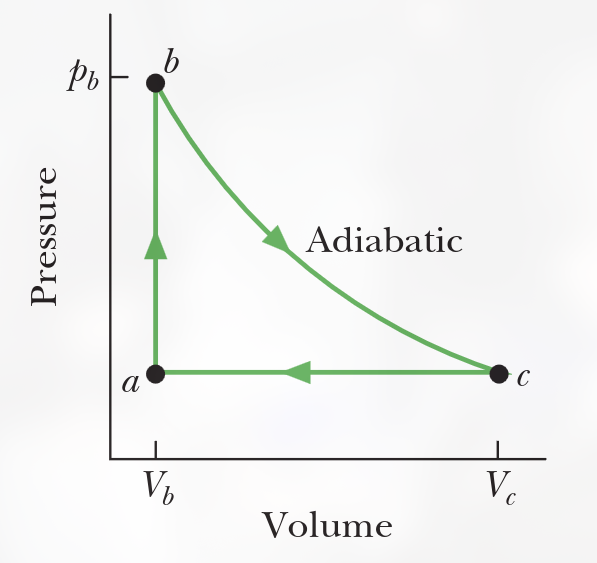
\includegraphics[width=0.4\linewidth]{images/33.png}
  \caption{Siklus gas ideal monoatomik (Gambar 20-29)}
\end{figure}}{}

\diketahui\ (dari Gambar 20-29: $a\to b$ volume tetap, $b\to c$ adiabatik, $c\to a$ tekanan tetap, dengan $p_a=p_c$ dan $V_a=V_b$)
\begin{align*}
n &= \SI{1,00}{\mole},&
p_b &= \SI{10,0}{\atm}=\SI{1,013e6}{\pascal},\\
V_b &= \SI{1,00e-3}{\metre\cubed},&
V_c &= 8{,}00V_b,\\
\gamma &= \tfrac53.
\end{align*}
\ditanya\ (a) $Q_{\text{masuk}}$; (b) $Q_{\text{keluar}}$; (c) $W$; (d) $\varepsilon$.

\konsep\ Kalor hanya masuk pada $a\to b$ ($Q=nC_V\Delta T$) dan hanya keluar pada $c\to a$ ($Q=nC_p\Delta T$); $b\to c$ adiabatik ($Q=0$). Usaha total $W=Q_{\text{masuk}}-|Q_{\text{keluar}}|$ dan $\varepsilon=W/Q_{\text{masuk}}$.

\penyelesaian

\noindent\textbf{Keadaan gas}
\begin{align*}
p_c &= p_b\left(\frac{V_b}{V_c}\right)^{\gamma} = (\SI{10,0}{\atm})\,8^{-5/3} = \frac{\SI{10,0}{\atm}}{32}=\SI{0,3125}{\atm}=p_a,\\
T_b &= \frac{p_bV_b}{nR}=\frac{(\SI{1,013e6}{\pascal})(\SI{1,00e-3}{\metre\cubed})}{(1{,}00)(8{,}314)}=\SI{121,8}{\kelvin},\\
T_a &= T_b\frac{p_a}{p_b}=\frac{T_b}{32}=\SI{3,81}{\kelvin},\qquad
T_c = T_b\frac{p_cV_c}{p_bV_b}=\frac{T_b}{4}=\SI{30,5}{\kelvin}.
\end{align*}

\noindent\textbf{(a) Kalor masuk ($a\to b$)}
\begin{align*}
Q_{ab} &= nC_V(T_b-T_a) = (1{,}00)(\tfrac32)(8{,}314)(121{,}8-3{,}81)\,\si{\joule} = \SI{1,47e3}{\joule}.
\end{align*}

\noindent\textbf{(b) Kalor keluar ($c\to a$)}
\begin{align*}
Q_{ca} &= nC_p(T_a-T_c) = (1{,}00)(\tfrac52)(8{,}314)(3{,}81-30{,}5)\,\si{\joule} = -\SI{554}{\joule},
\end{align*}
sehingga energi yang meninggalkan gas sebagai kalor adalah \SI{554}{\joule}.

\noindent\textbf{(c) Usaha total}
\begin{align*}
W &= Q_{ab}+Q_{ca} = \SI{1,47e3}{\joule}-\SI{554}{\joule} = \SI{918}{\joule}.
\end{align*}

\noindent\textbf{(d) Efisiensi}
\begin{align*}
\varepsilon &= \frac{W}{Q_{ab}} = \frac{\SI{918}{\joule}}{\SI{1,47e3}{\joule}} = 0{,}624.
\end{align*}
\begin{jawaban}
(a) $\SI{1,47}{\kilo\joule}$ \quad (b) $\SI{0,554}{\kilo\joule}$ \quad (c) $\SI{0,918}{\kilo\joule}$ \quad (d) $\varepsilon\approx62{,}4\%$.
\end{jawaban}

% ---------------------------------------------------------------------
\soal{35}
Siklus pada Gambar 20-31 menggambarkan kerja mesin pembakaran dalam berbahan bensin. Volume $V_3=4{,}00V_1$. Anggap campuran bensin--udara yang masuk adalah gas ideal dengan $\gamma=\num{1,30}$. Berapa perbandingan (a) $T_2/T_1$, (b) $T_3/T_1$, (c) $T_4/T_1$, (d) $p_3/p_1$, dan (e) $p_4/p_1$? (f) Berapa efisiensi mesin?

\IfFileExists{images/35.png}{%
\begin{figure}[H]
  \centering
  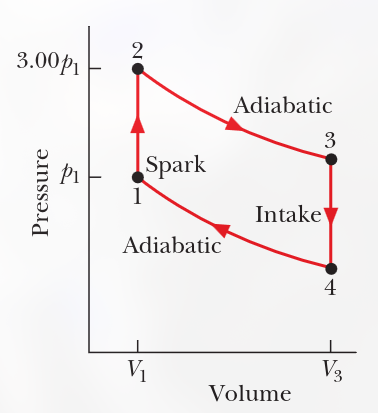
\includegraphics[width=0.4\linewidth]{images/35.png}
  \caption{Siklus mesin bensin (Gambar 20-31)}
\end{figure}}{}

\diketahui\ (dari Gambar 20-31: $1\to2$ volume tetap ("spark") hingga $p_2=3{,}00p_1$; $2\to3$ adiabatik; $3\to4$ volume tetap; $4\to1$ adiabatik)
\begin{align*}
V_3 &= V_4 = 4{,}00V_1,&
V_2 &= V_1,&
p_2 &= 3{,}00p_1,&
\gamma &= \num{1,30}.
\end{align*}
\ditanya\ $T_2/T_1$, $T_3/T_1$, $T_4/T_1$, $p_3/p_1$, $p_4/p_1$, dan efisiensi $\varepsilon$.

\konsep\ Hukum gas ideal $pV/T=\text{konstan}$; proses adiabatik: $TV^{\gamma-1}=\text{konstan}$ dan $pV^{\gamma}=\text{konstan}$. Efisiensi $\varepsilon=1-|Q_{\text{keluar}}|/Q_{\text{masuk}}$, dengan kalor hanya dipertukarkan pada proses volume tetap ($Q=nC_V\Delta T$).

\penyelesaian

\noindent\textbf{(a)} $1\to2$ pada volume tetap:
\begin{align*}
\frac{T_2}{T_1} &= \frac{p_2}{p_1} = 3{,}00.
\end{align*}

\noindent\textbf{(b), (d)} $2\to3$ adiabatik:
\begin{align*}
\frac{T_3}{T_2} &= \left(\frac{V_2}{V_3}\right)^{\gamma-1}=4^{-0{,}30}=0{,}660
\;\Rightarrow\; \frac{T_3}{T_1}=3{,}00(0{,}660)=1{,}98,\\
\frac{p_3}{p_2} &= \left(\frac{V_2}{V_3}\right)^{\gamma}=4^{-1{,}30}=0{,}165
\;\Rightarrow\; \frac{p_3}{p_1}=3{,}00(0{,}165)=0{,}495.
\end{align*}

\noindent\textbf{(c), (e)} $4\to1$ adiabatik ($V_4=V_3=4V_1$ ke $V_1$):
\begin{align*}
\frac{T_4}{T_1} &= \left(\frac{V_1}{V_4}\right)^{\gamma-1}=4^{-0{,}30}=0{,}660,\\
\frac{p_4}{p_1} &= \left(\frac{V_1}{V_4}\right)^{\gamma}=4^{-1{,}30}=0{,}165.
\end{align*}

\noindent\textbf{(f) Efisiensi}
\begin{align*}
Q_{\text{masuk}} &= nC_V(T_2-T_1) = nC_VT_1(3{,}00-1) = 2{,}00\,nC_VT_1,\\
|Q_{\text{keluar}}| &= nC_V(T_3-T_4) = nC_VT_1(1{,}98-0{,}660) = 1{,}32\,nC_VT_1,\\
\varepsilon &= 1-\frac{1{,}32}{2{,}00} = 0{,}340
\quad\left(=1-4^{-0{,}30}\right).
\end{align*}
\begin{jawaban}
(a) $3{,}00$ \quad (b) $1{,}98$ \quad (c) $0{,}660$ \quad (d) $0{,}495$ \quad (e) $0{,}165$ \quad (f) $\varepsilon\approx34\%$.
\end{jawaban}

% ---------------------------------------------------------------------
\soal{57}
Suhu \SI{1,00}{\mole} gas ideal monoatomik dinaikkan secara reversibel dari \SI{300}{\kelvin} menjadi \SI{400}{\kelvin} dengan volume dijaga tetap. Berapa perubahan entropi gas?

\diketahui
\begin{align*}
n &= \SI{1,00}{\mole},&
T_i &= \SI{300}{\kelvin},&
T_f &= \SI{400}{\kelvin},&
V &= \text{konstan}.
\end{align*}
\ditanya\ $\Delta S$.

\konsep\ Pada volume tetap, $dQ=nC_V\,dT$ dengan $C_V=\tfrac32R$ (monoatomik), sehingga $\Delta S=\displaystyle\int_{T_i}^{T_f}\frac{nC_V\,dT}{T}=nC_V\ln\frac{T_f}{T_i}$.

\penyelesaian
\begin{align*}
\Delta S &= n\left(\tfrac32R\right)\ln\frac{T_f}{T_i}
= (1{,}00)(\tfrac32)(\SI{8,31}{\joule\per\mole\per\kelvin})\ln\frac{400}{300}
= \SI{3,59}{\joule\per\kelvin}.
\end{align*}
\begin{jawaban}
\[
\boxed{\Delta S\approx\SI{3,59}{\joule\per\kelvin}}
\]
\end{jawaban}

% ---------------------------------------------------------------------
\soal{59}
Sampel air bermassa \SI{0,600}{\kilo\gram} mula-mula berupa es bersuhu \SI{-20}{\celsius}. Berapa perubahan entropi sampel jika suhunya dinaikkan menjadi \SI{40}{\celsius}?

\diketahui\ (Tabel 18-3 dan 18-4)
\begin{align*}
m &= \SI{0,600}{\kilo\gram},&
c_{\text{es}} &= \SI{2220}{\joule\per\kilo\gram\per\kelvin},&
c_{\text{air}} &= \SI{4190}{\joule\per\kilo\gram\per\kelvin},&
L_F &= \SI{333}{\kilo\joule\per\kilo\gram}.
\end{align*}
\ditanya\ $\Delta S_{\text{total}}$ dari \SI{-20}{\celsius} (es) ke \SI{40}{\celsius} (air).

\konsep\ Entropi adalah fungsi keadaan, sehingga perubahannya dihitung lewat tiga proses reversibel: (1) es dipanaskan $\SI{253}{\kelvin}\to\SI{273}{\kelvin}$, $\Delta S_1=mc_{\text{es}}\ln\dfrac{T_2}{T_1}$; (2) es melebur pada $\SI{273}{\kelvin}$, $\Delta S_2=\dfrac{mL_F}{T}$; (3) air dipanaskan $\SI{273}{\kelvin}\to\SI{313}{\kelvin}$, $\Delta S_3=mc_{\text{air}}\ln\dfrac{T_3}{T_2}$.

\penyelesaian
\begin{align*}
\Delta S_1 &= (0{,}600)(2220)\ln\frac{273}{253} = \SI{101}{\joule\per\kelvin},\\
\Delta S_2 &= \frac{(0{,}600)(\SI{3,33e5}{\joule\per\kilo\gram})}{\SI{273}{\kelvin}} = \SI{731}{\joule\per\kelvin},\\
\Delta S_3 &= (0{,}600)(4190)\ln\frac{313}{273} = \SI{344}{\joule\per\kelvin},\\
\Delta S_{\text{total}} &= 101+731+344 = \SI{1,18e3}{\joule\per\kelvin}.
\end{align*}
\begin{jawaban}
\[
\boxed{\Delta S\approx\SI{1,18e3}{\joule\per\kelvin}}
\]
\end{jawaban}

% ---------------------------------------------------------------------
\soal{66}
Sebuah pendingin ideal melakukan usaha \SI{150}{\joule} untuk mengambil \SI{560}{\joule} kalor dari kompartemen dinginnya. (a) Berapa koefisien kinerja pendingin? (b) Berapa kalor per siklus yang dibuang ke dapur?

\diketahui
\begin{align*}
|W| &= \SI{150}{\joule},&
|Q_C| &= \SI{560}{\joule}.
\end{align*}
\ditanya\ (a) $K$; (b) $|Q_H|$.

\konsep\ $K=\dfrac{|Q_C|}{|W|}$ dan kekekalan energi pada satu siklus: $|Q_H|=|Q_C|+|W|$.

\penyelesaian

\noindent\textbf{(a) Koefisien kinerja}
\begin{align*}
K &= \frac{|Q_C|}{|W|} = \frac{\SI{560}{\joule}}{\SI{150}{\joule}} = 3{,}73.
\end{align*}

\noindent\textbf{(b) Kalor yang dibuang ke dapur}
\begin{align*}
|Q_H| &= |Q_C|+|W| = \SI{560}{\joule}+\SI{150}{\joule} = \SI{710}{\joule}.
\end{align*}
\begin{jawaban}
(a) $K\approx3{,}73$ \quad (b) $|Q_H|=\SI{710}{\joule}$.
\end{jawaban}

% ---------------------------------------------------------------------
\soal{72}
Hitung efisiensi pembangkit listrik berbahan bakar fosil yang membakar $380$ ton metrik batu bara tiap jam untuk menghasilkan kerja berguna dengan laju \SI{750}{\mega\watt}. Kalor pembakaran batu bara (kalor akibat pembakarannya) adalah \SI{28}{\mega\joule\per\kilo\gram}.

\diketahui\ ($1$ ton metrik $=\SI{1000}{\kilo\gram}$)
\begin{align*}
\frac{m}{t} &= \frac{380\times10^3\,\si{\kilo\gram}}{3600\,\si{\second}},&
L_c &= \SI{28}{\mega\joule\per\kilo\gram},&
P_{\text{keluar}} &= \SI{750}{\mega\watt}.
\end{align*}
\ditanya\ Efisiensi $\varepsilon$.

\konsep\ Efisiensi $\varepsilon=\dfrac{P_{\text{keluar}}}{P_{\text{masuk}}}$, dengan laju energi masuk dari pembakaran $P_{\text{masuk}}=\dfrac{m}{t}L_c$.

\penyelesaian
\begin{align*}
\frac{m}{t} &= \frac{\SI{3,80e5}{\kilo\gram}}{3600\,\si{\second}} = \SI{105,6}{\kilo\gram\per\second},\\
P_{\text{masuk}} &= \frac{m}{t}L_c = (\SI{105,6}{\kilo\gram\per\second})(\SI{28e6}{\joule\per\kilo\gram}) = \SI{2,96e9}{\watt},\\
\varepsilon &= \frac{P_{\text{keluar}}}{P_{\text{masuk}}} = \frac{\SI{750e6}{\watt}}{\SI{2,96e9}{\watt}} = 0{,}254.
\end{align*}
\begin{jawaban}
\[
\boxed{\varepsilon\approx25{,}4\%}
\]
\end{jawaban}

% ---------------------------------------------------------------------
\soal{74}
Mesin Carnot yang reservoir bersuhu tingginya \SI{400}{\kelvin} memiliki efisiensi \SI{30,0}{\percent}. Berapa suhu reservoir bersuhu rendah harus diubah agar efisiensinya naik menjadi \SI{40,0}{\percent}?

\diketahui
\begin{align*}
T_H &= \SI{400}{\kelvin},&
\varepsilon_1 &= 0{,}300,&
\varepsilon_2 &= 0{,}400.
\end{align*}
\ditanya\ Perubahan suhu reservoir rendah $\Delta T_C$.

\konsep\ Efisiensi mesin Carnot $\varepsilon=1-\dfrac{T_C}{T_H}$, sehingga $T_C=T_H(1-\varepsilon)$.

\penyelesaian
\begin{align*}
T_{C1} &= T_H(1-\varepsilon_1) = (\SI{400}{\kelvin})(0{,}700) = \SI{280}{\kelvin},\\
T_{C2} &= T_H(1-\varepsilon_2) = (\SI{400}{\kelvin})(0{,}600) = \SI{240}{\kelvin},\\
\Delta T_C &= T_{C2}-T_{C1} = -\SI{40}{\kelvin}.
\end{align*}
\begin{jawaban}
\[
\boxed{\Delta T_C = -\SI{40,0}{\kelvin}}
\]
(suhu reservoir rendah harus \textit{diturunkan} sebesar \SI{40,0}{\kelvin}).
\end{jawaban}

% ---------------------------------------------------------------------
\soal{76}
Gambar 20-36 memperlihatkan siklus Carnot pada diagram $T$--$S$ dengan skala ditetapkan oleh $S_s=\SI{0,60}{\joule\per\kelvin}$. Untuk satu siklus penuh, tentukan (a) perpindahan kalor total dan (b) usaha total yang dilakukan sistem.

\IfFileExists{images/76.png}{%
\begin{figure}[H]
  \centering
  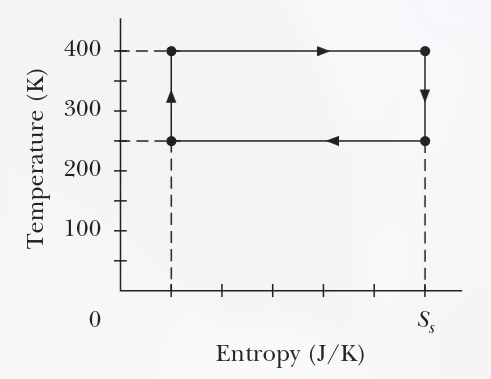
\includegraphics[width=0.45\linewidth]{images/76.png}
  \caption{Siklus Carnot pada diagram $T$--$S$ (Gambar 20-36)}
\end{figure}}{}

\diketahui\ (dibaca dari Gambar 20-36: siklus berbentuk persegi panjang dengan $T_H=\SI{400}{\kelvin}$ di atas dan $T_C=\SI{250}{\kelvin}$ di bawah; entropi berubah dari $\SI{0,10}{\joule\per\kelvin}$ sampai $S_s=\SI{0,60}{\joule\per\kelvin}$, karena tiap tanda skala sebesar $S_s/6$)
\begin{align*}
T_H &= \SI{400}{\kelvin},&
T_C &= \SI{250}{\kelvin},&
\Delta S &= \SI{0,60}{\joule\per\kelvin}-\SI{0,10}{\joule\per\kelvin}=\SI{0,50}{\joule\per\kelvin}.
\end{align*}
\ditanya\ (a) $Q_{\text{total}}$; (b) $W_{\text{total}}$.

\konsep\ Pada diagram $T$--$S$, kalor pada proses isotermal adalah $Q=T\,\Delta S$, dan proses adiabatik reversibel ($\Delta S=0$) tidak melibatkan kalor. Untuk satu siklus penuh $\Delta E_{\text{int}}=0$, jadi $W=Q_{\text{total}}$ (sama dengan luas persegi panjang).

\penyelesaian

\noindent\textbf{(a) Kalor total}
\begin{align*}
Q_H &= T_H\,\Delta S = (\SI{400}{\kelvin})(\SI{0,50}{\joule\per\kelvin}) = \SI{200}{\joule}\ \text{(masuk)},\\
Q_C &= -T_C\,\Delta S = -(\SI{250}{\kelvin})(\SI{0,50}{\joule\per\kelvin}) = -\SI{125}{\joule}\ \text{(keluar)},\\
Q_{\text{total}} &= Q_H+Q_C = (T_H-T_C)\,\Delta S = (\SI{150}{\kelvin})(\SI{0,50}{\joule\per\kelvin}) = \SI{75}{\joule}.
\end{align*}

\noindent\textbf{(b) Usaha total}
\begin{align*}
W_{\text{total}} &= Q_{\text{total}} = \SI{75}{\joule}.
\end{align*}
\begin{jawaban}
(a) $Q_{\text{total}}=\SI{75}{\joule}$ \quad (b) $W_{\text{total}}=\SI{75}{\joule}$.
\end{jawaban}

% ---------------------------------------------------------------------
\soal{78}
Sebuah mesin Carnot berdaya \SI{500}{\watt} beroperasi di antara reservoir kalor bersuhu \SI{100}{\celsius} dan \SI{60,0}{\celsius}. Hitung (a) laju kalor masuk dan (b) laju kalor buang (kalor yang dibuang per satuan waktu).

\diketahui
\begin{align*}
P &= \SI{500}{\watt},&
T_H &= \SI{100}{\celsius}=\SI{373}{\kelvin},&
T_C &= \SI{60,0}{\celsius}=\SI{333}{\kelvin}.
\end{align*}
\ditanya\ (a) Laju kalor masuk $|Q_H|/t$; (b) laju kalor buang $|Q_C|/t$.

\konsep\ Efisiensi mesin Carnot $\varepsilon_C=1-\dfrac{T_C}{T_H}$ (suhu dalam kelvin) dan $\varepsilon=\dfrac{P}{|Q_H|/t}$. Dari kekekalan energi, $|Q_H|/t=P+|Q_C|/t$.

\penyelesaian

\noindent\textbf{(a) Laju kalor masuk}
\begin{align*}
\varepsilon_C &= 1-\frac{T_C}{T_H} = 1-\frac{333{,}15}{373{,}15} = 0{,}1072,\\
\frac{|Q_H|}{t} &= \frac{P}{\varepsilon_C} = \frac{\SI{500}{\watt}}{0{,}1072} = \SI{4,66e3}{\watt}.
\end{align*}

\noindent\textbf{(b) Laju kalor buang}
\begin{align*}
\frac{|Q_C|}{t} &= \frac{|Q_H|}{t}-P = \SI{4,66e3}{\watt}-\SI{500}{\watt} = \SI{4,16e3}{\watt}.
\end{align*}
\begin{jawaban}
(a) $\SI{4,66e3}{\watt}$ \quad (b) $\SI{4,16e3}{\watt}$.
\end{jawaban}

% ---------------------------------------------------------------------
\soal{79}
Pada sebuah pendingin nyata, kumparan bersuhu rendah berada pada \SI{-13}{\celsius} dan gas terkompresi di kondensor berada pada \SI{26}{\celsius}. Berapa koefisien kinerja teoretisnya?

\diketahui
\begin{align*}
T_C &= \SI{-13}{\celsius}=\SI{260}{\kelvin},&
T_H &= \SI{26}{\celsius}=\SI{299}{\kelvin}.
\end{align*}
\ditanya\ Koefisien kinerja teoretis $K_C$.

\konsep\ Koefisien kinerja maksimum (teoretis) adalah koefisien kinerja pendingin Carnot, $K_C=\dfrac{T_C}{T_H-T_C}$, dengan suhu dalam kelvin.

\penyelesaian
\begin{align*}
K_C &= \frac{T_C}{T_H-T_C} = \frac{\SI{260}{\kelvin}}{\SI{299}{\kelvin}-\SI{260}{\kelvin}} = 6{,}67.
\end{align*}
\begin{jawaban}
\[
\boxed{K_C\approx 6{,}67}
\]
\end{jawaban}

% ======================================================================
%% KESIMPULAN
% ======================================================================
\clearpage
\phantomsection
\addcontentsline{toc}{section}{Kesimpulan}
\section*{Kesimpulan}

Dokumen ini menyusun penyelesaian soal-soal terpilih dari \textit{Fundamentals of Physics}
\cite{halliday} Bab 14 sampai Bab 20. Setiap bab diawali ringkasan prinsip dan rumus utama,
kemudian soal diselesaikan dengan pola \textit{diketahui}, \textit{ditanya}, \textit{konsep},
dan \textit{penyelesaian}. Kesimpulan tiap bab adalah sebagai berikut.

\paragraph{Bab 14 (Fluida).}
Lima belas soal terpilih diselesaikan dengan empat prinsip, yaitu tekanan hidrostatik,
prinsip Pascal, prinsip Archimedes, serta persamaan kontinuitas dan Bernoulli.
Pada prinsip Pascal (Soal 28), gaya kecil $f \approx \SI{1,03e2}{\newton}$ pada piston berdiameter
$\SI{3,80}{\centi\metre}$ dapat menyeimbangkan gaya $\SI{20,0}{\kilo\newton}$ pada piston berdiameter
$\SI{53,0}{\centi\metre}$. Pada prinsip Archimedes, gaya apung sama dengan selisih gaya tekan
pada sisi bawah dan sisi atas benda (Soal 32, $F_b \approx \SI{2,18e3}{\newton}$) dan menentukan
berat semu benda (Soal 33, 79, 80, dan 86). Pada Soal 88, tekanan pada kedalaman
$\SI{2,22}{\kilo\metre}$ mencapai sekitar $\SI{2,23e7}{\pascal}$. Pada aliran fluida, persamaan
kontinuitas dan Bernoulli menghubungkan kelajuan dan tekanan: tabung pitot (Soal 62 dan 63),
pipa menyempit (Soal 64), venturimeter (Soal 65 dan 66), semburan dari lubang tangki
(Soal 71, $x \approx \SI{0,35}{\metre}$), drainase air hujan (Soal 72), dan sifon (Soal 83,
$v_C \approx \SI{3,2}{\metre\per\second}$). Secara umum, tekanan fluida bertambah dengan kedalaman, dan
di mana kelajuan aliran bertambah, tekanannya berkurang.

\paragraph{Bab 15 (Osilasi).}
Soal-soal bab ini bertumpu pada gerak harmonik sederhana, yaitu periode dan frekuensi
ditentukan oleh sifat sistem (misalnya $T = 2\pi\sqrt{m/k}$ pada pegas dan $T = 2\pi\sqrt{L/g}$ pada
bandul), sedangkan energi mekanik total tetap dan hanya berpindah antara energi kinetik dan
energi potensial.

\paragraph{Bab 16 (Gelombang I).}
Gelombang ditandai oleh bilangan gelombang, frekuensi sudut, dan laju gelombang
$v = \lambda f$. Pada tali, laju ditentukan oleh tegangan dan massa per satuan panjang, dan
superposisi gelombang menghasilkan interferensi serta gelombang berdiri dengan frekuensi
resonansi tertentu.

\paragraph{Bab 17 (Gelombang II).}
Bunyi adalah gelombang longitudinal yang lajunya bergantung pada modulus \textit{bulk} dan massa
jenis medium. Intensitas bunyi menurun terhadap kuadrat jarak, taraf intensitas dinyatakan
dalam desibel, dan pergeseran frekuensi akibat gerak sumber atau pendengar dijelaskan oleh
efek Doppler.

\paragraph{Bab 18 (Suhu, Kalor, dan Hukum Pertama Termodinamika).}
Perubahan suhu menimbulkan pemuaian dan perpindahan kalor, baik secara konduksi maupun
radiasi. Hukum Pertama Termodinamika, $\Delta E_{\text{int}} = Q - W$, menyatakan kekekalan energi
yang melibatkan kalor dan usaha.

\paragraph{Bab 19 (Teori Kinetik Gas).}
Sifat makroskopik gas ideal (tekanan dan suhu) dijelaskan oleh gerak molekul: suhu
sebanding dengan energi kinetik translasi rata-rata molekul. Energi dalam gas ideal
bergantung pada suhu dan kalor jenis molar, serta proses adiabatik mengikuti $pV^{\gamma}=\text{konstan}$.

\paragraph{Bab 20 (Entropi dan Hukum Kedua Termodinamika).}
Entropi sistem tertutup tidak pernah berkurang. Hukum Kedua membatasi efisiensi mesin kalor,
dan efisiensi tertinggi dicapai oleh mesin Carnot, $\varepsilon_C = 1 - T_C/T_H$.

% ======================================================================
%% DAFTAR PUSTAKA
% ======================================================================
\clearpage
\phantomsection
\addcontentsline{toc}{section}{Daftar Pustaka}
\begin{thebibliography}{9}
\bibitem{halliday}
Halliday, D., Resnick, R., \& Walker, J. (2014).
\textit{Fundamentals of Physics} (10th ed.). Hoboken, NJ: John Wiley \& Sons.
\end{thebibliography}

\end{document}
